\section{Results}
Overview of scores with ref to Fig. \ref{fig:scores}

\subsection{Climate}
\hilight{Alistiar - chech how much of this is covered in your evaluation paper}
\begin{itemize}
    \item Broad scale patterns are cool
    \item Sahel, Eastern Amazon and India are too dry and hot.
    \item Dryness in India is due to missing wet season precipitation (Fig. xx \ref{fig:ClimateSeasonUKESMmaps}), in areas of very high concentration in precipitation ($C_{mod} \rightarrow 1$, Fig. \ref{fig:ClimateSeasonObsMaps}) 
    \item There is too much annual precipitation in much of the Southern Hemisphere, particularly south of the Amazon, in the Ceraado and Catinga Savanna and woodland and southern Africa.
    \item UKESM captures the precip, tempuarture \label{fig:ClimateAAMaps} and precip biomadiaity \ref{fig:ClimateSeasonUKESMmaps} of the Eurasian Steppe
    \item biases in MAT and MAT seem to be correclated - where its to wet its too hot and vice versa. Australia is the exception, where there is a ~ 2 degree warm bias corrisiciding with a 10-200 mm/yr wet biases in an areas that typically reciences very liuttle precipitation \label{fig:ClimateAAMaps}. Precicpitation modality, timing and conceptration are reproduced by UKESM, though their is a stronger seasonal cycle in tempertaure \ref{fig:ClimateSeasonUKESMmaps}, with too hot summers (Fig. xx)
\end{itemize}

\begin{itemize}
    \item{Wet bias: Vs CMAP bias = 0.321 mm/day. Vs Fluxnet bias = 0.000661 mm/day. Vs GPCC = 0.189. Vs GPCP2 = 0.0332
Largest bias is vs CMAP. Wet bias over Andes, southern Brazil, China. Dry bias over India. \ref{fig:ClimateAAMaps}}
    \item Biases: too high. Vs CERES = 9.86 W/m2. vs Fluxnet = 13.5W/m2. Vs GWEX = 10.2 W/m2. vs WRMC = 8.79 W/m2
\end{itemize}

\begin{figure*}[t]
    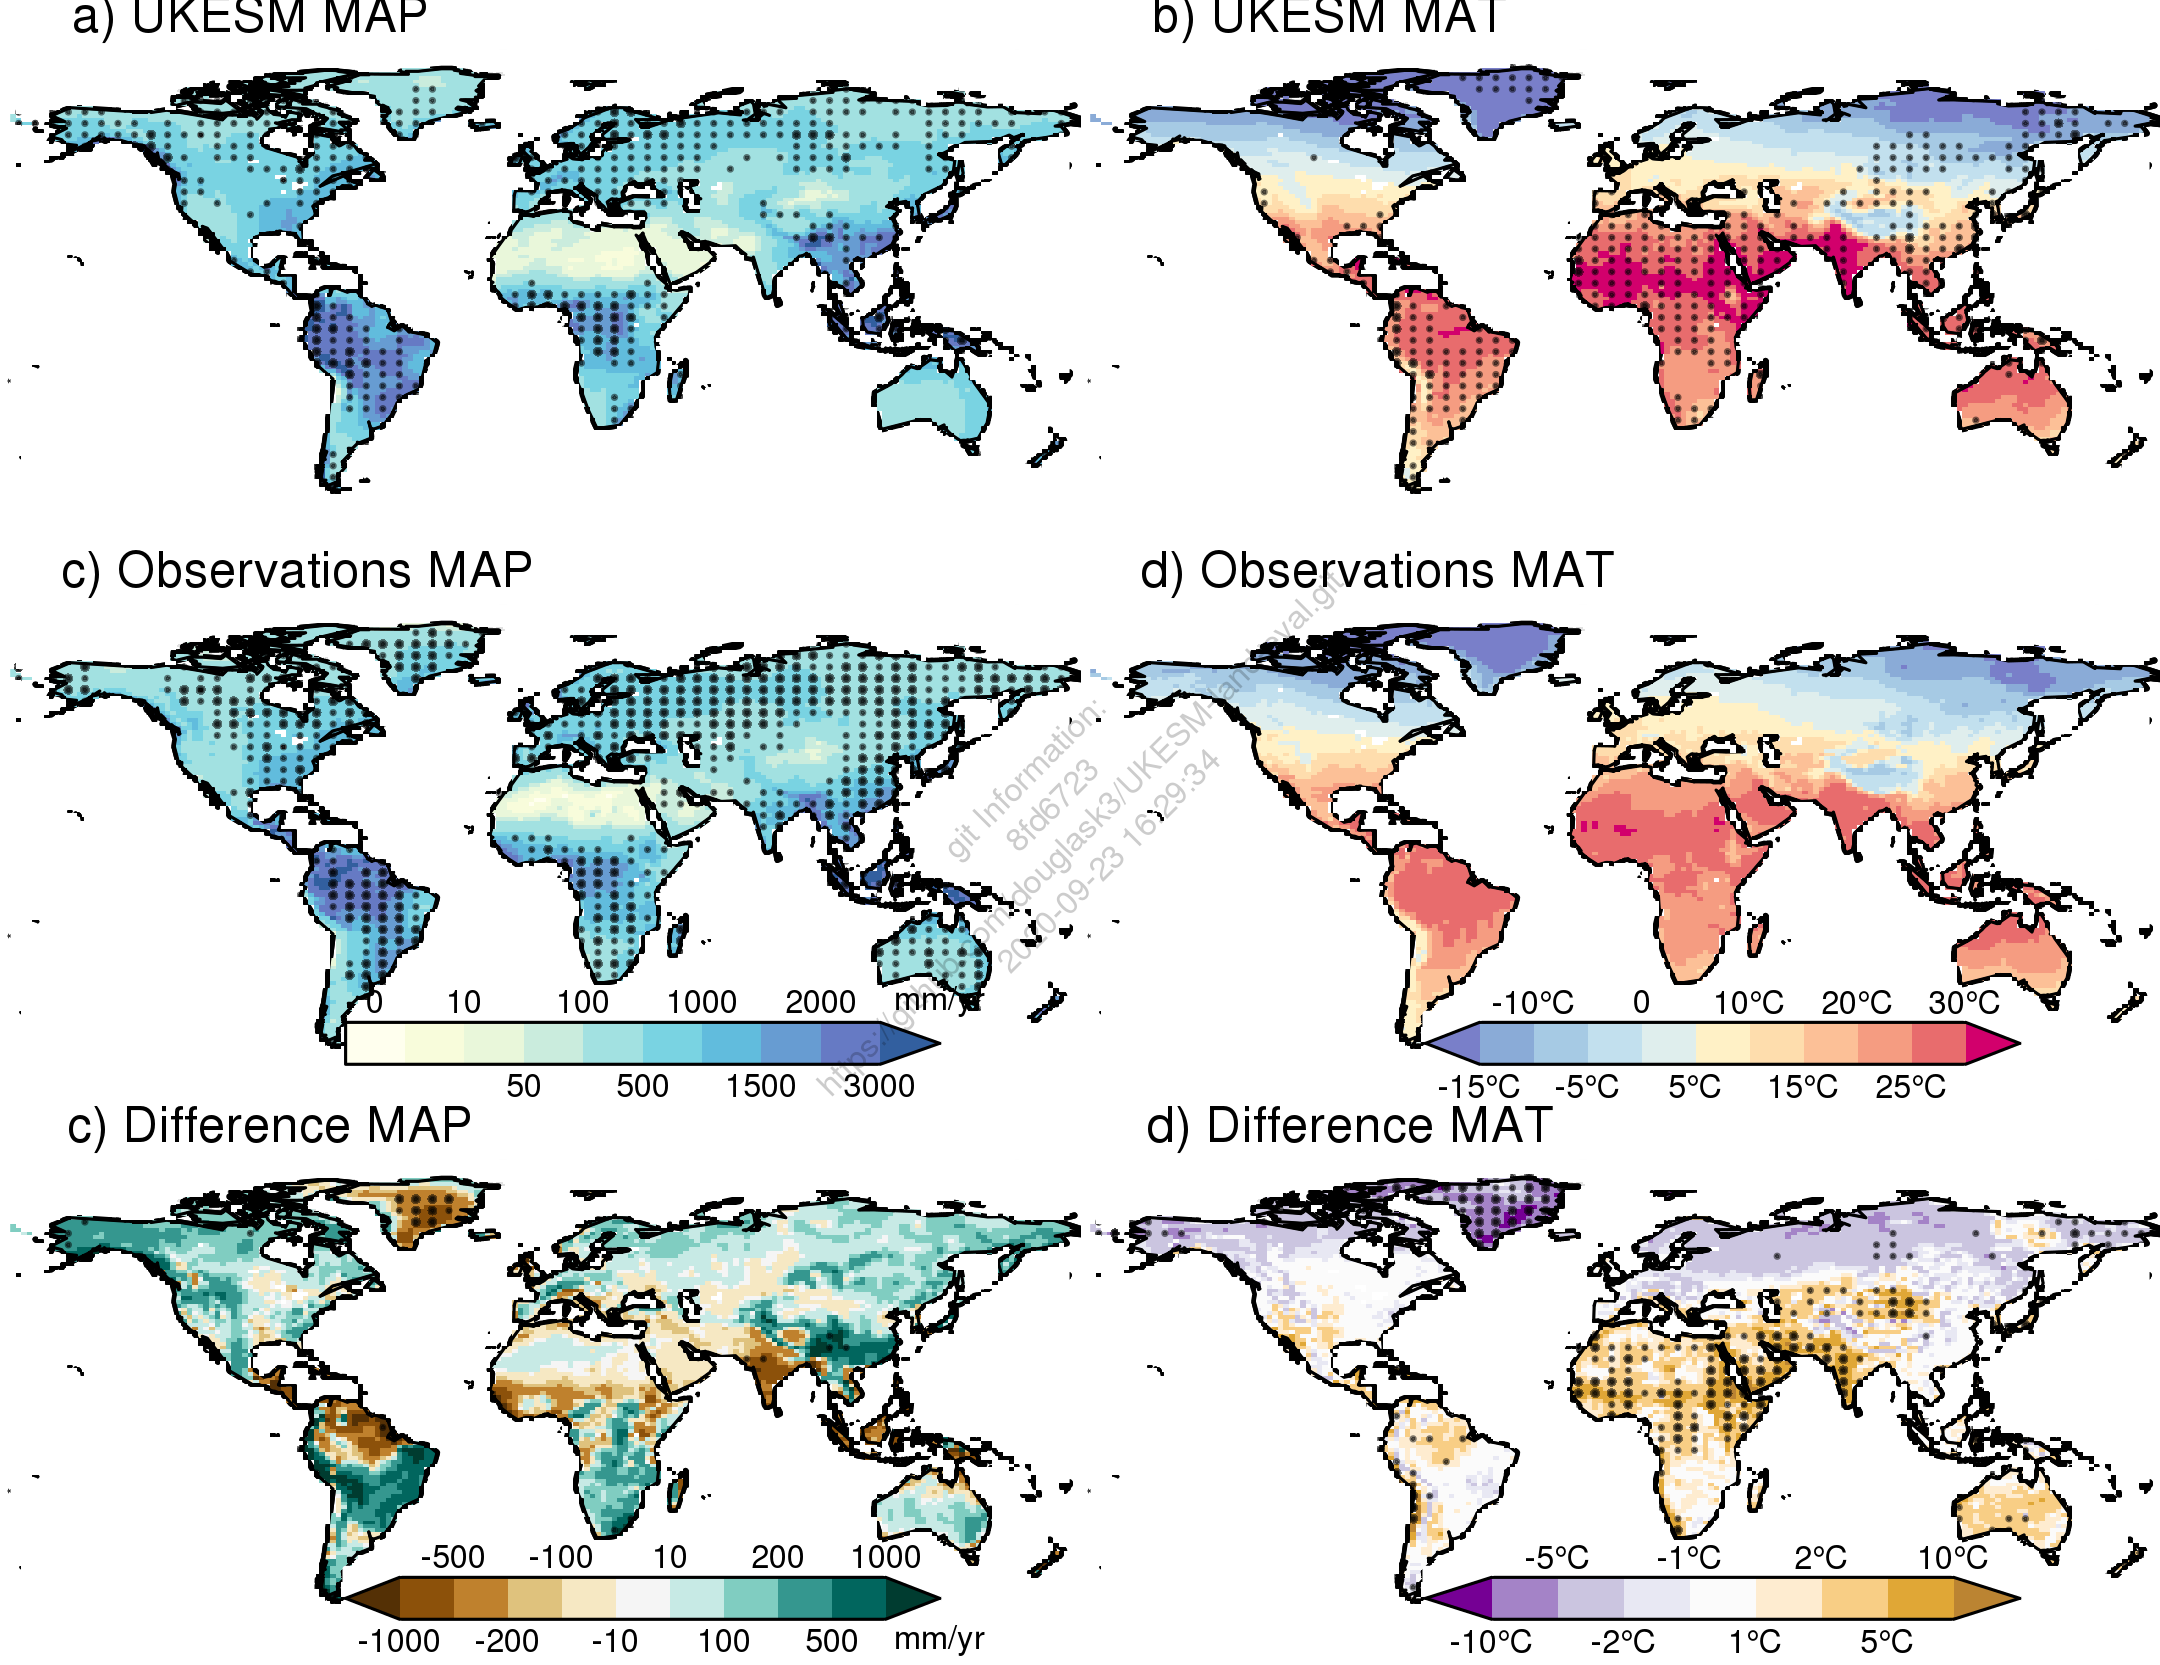
\includegraphics[width=12cm]{figs/Climate/annual_average_clims.png}
    \caption{Climate comparison \label{fig:ClimateAAMaps}}
\end{figure*}

\begin{figure*}[t]
    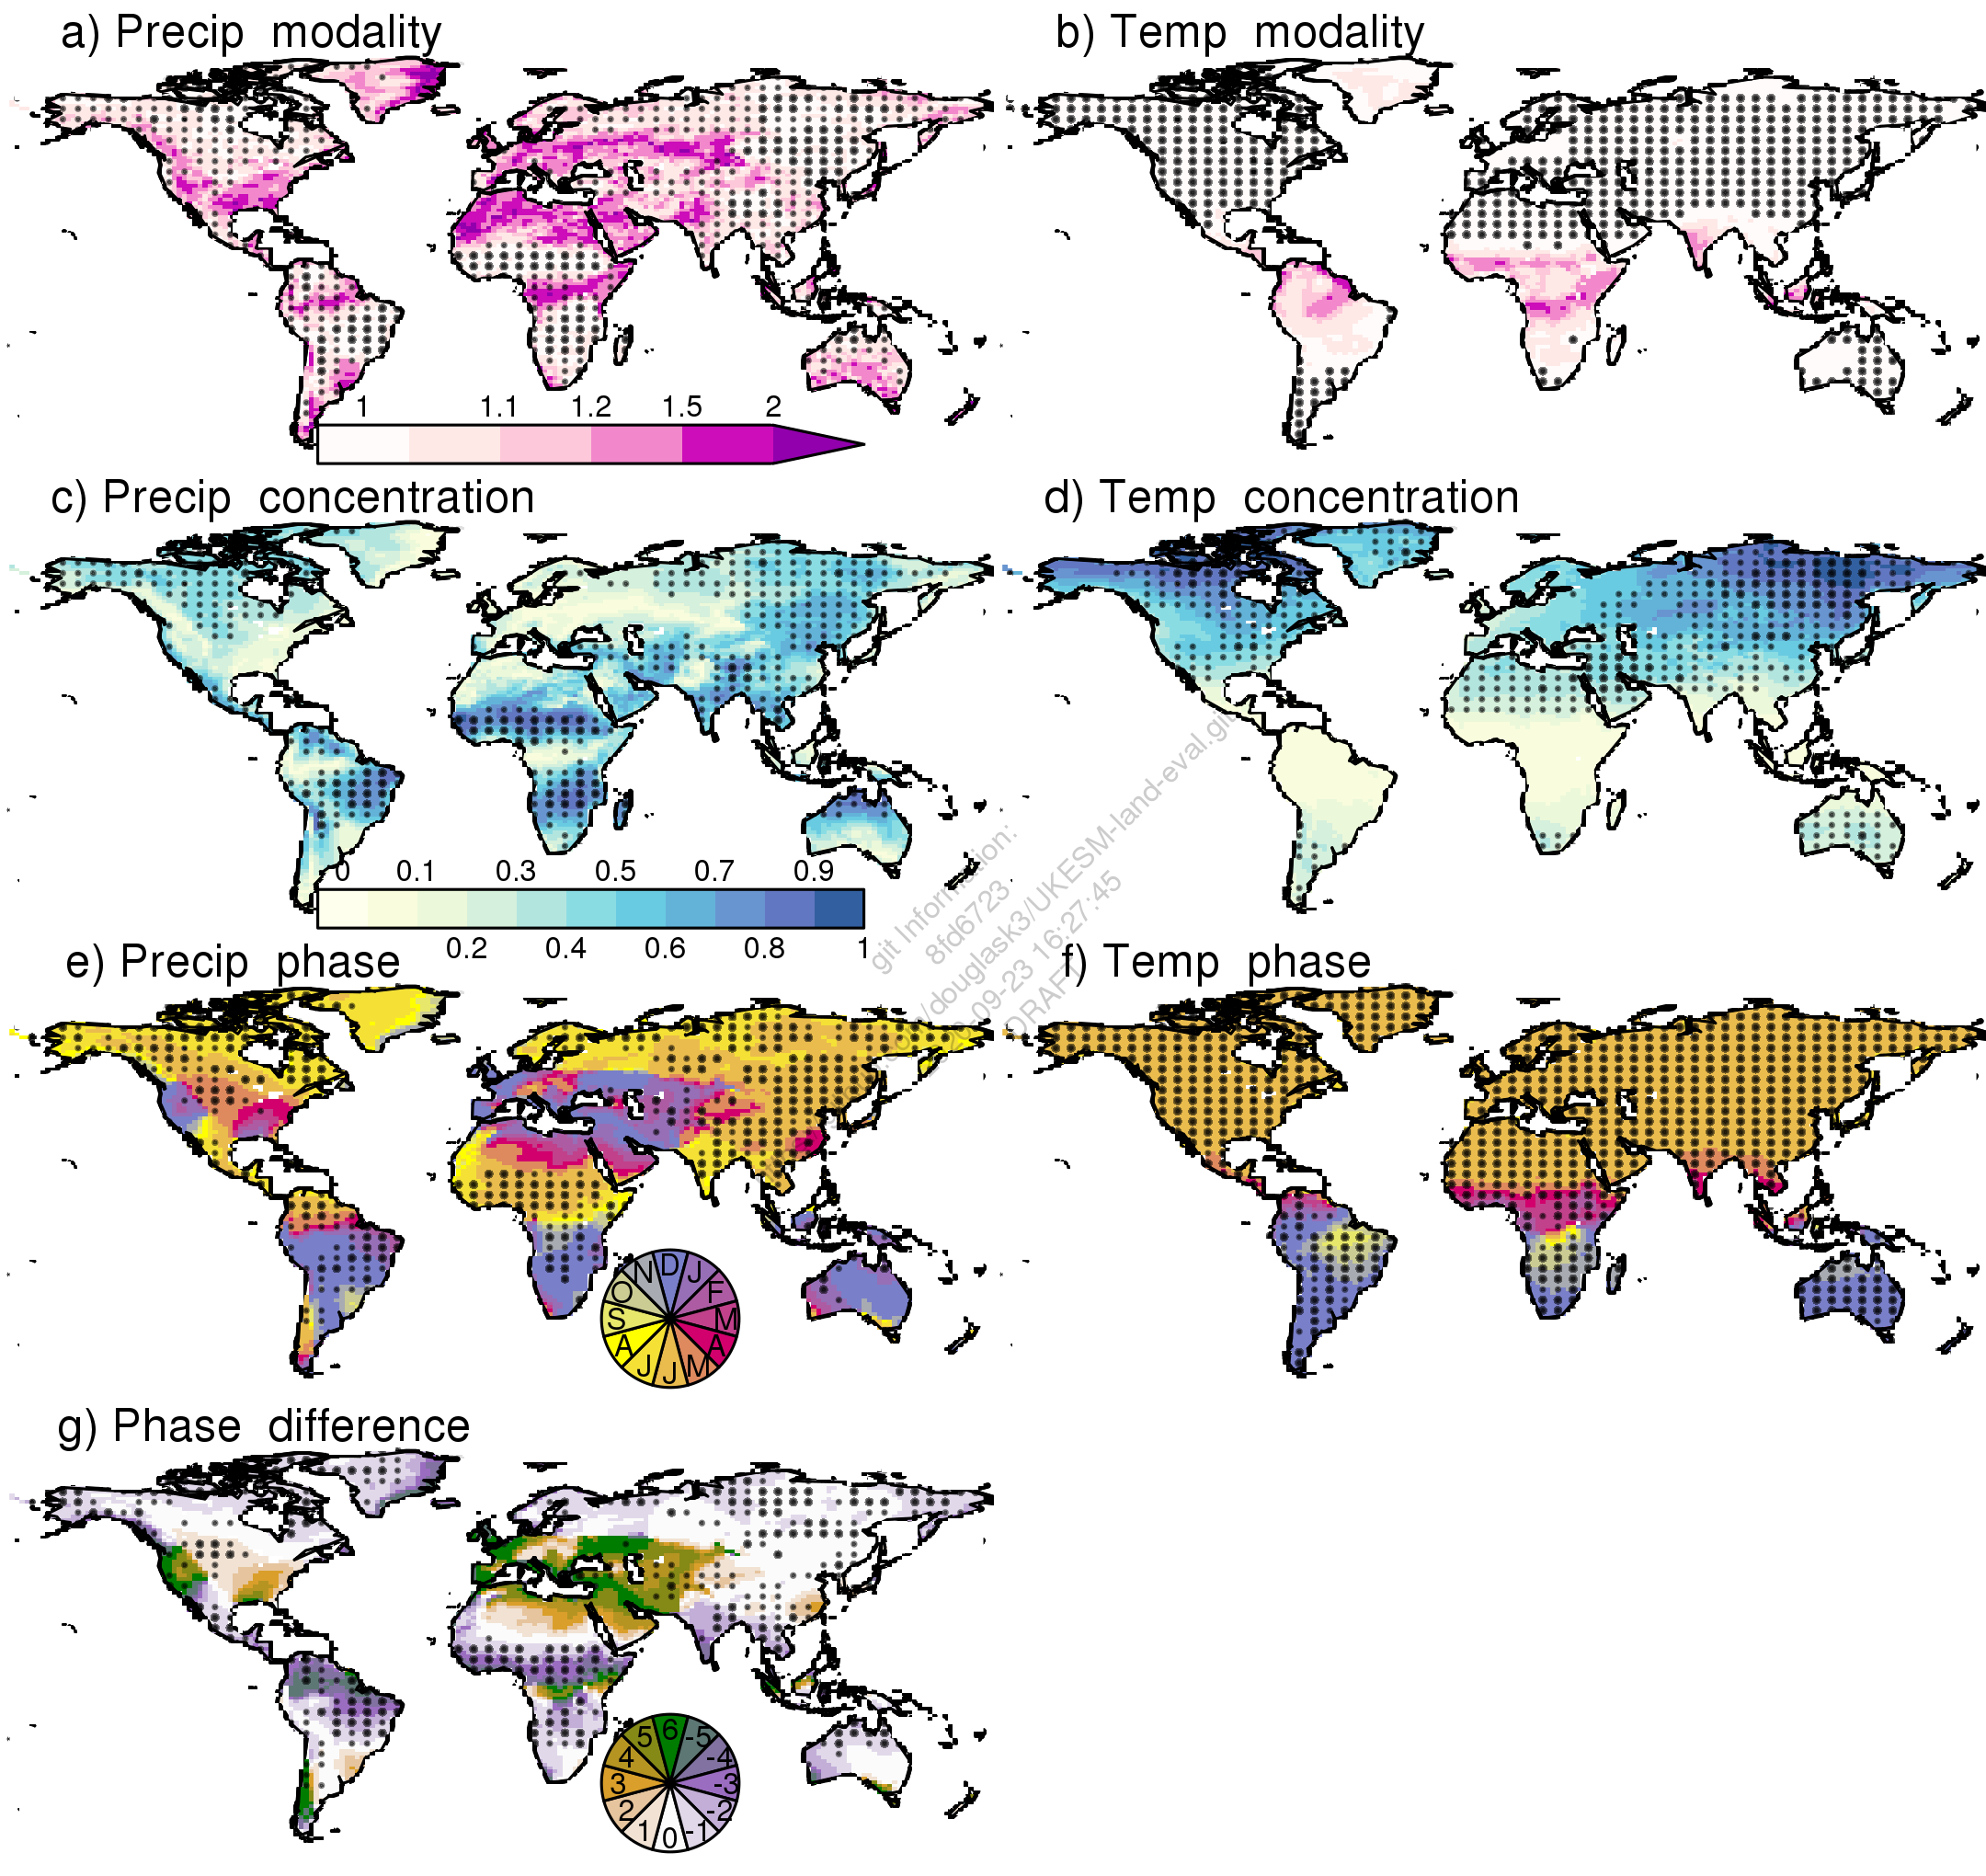
\includegraphics[width=12cm]{figs/Climate/climStuff-UKESM.png}
    \caption{UKESM precipitation (a, c, e) and temperature (b, d, f) seasonal metrics. a,b) modality; c,d) concentration; e,f) phase. g) shows the difference in phase between precip and temperature. Positive shows precip leading temperature, negative precip lagging temperature. Dots show smaller spread (higher confidence) across ensemble members. <<define>>  \label{fig:ClimateSeasonUKESMmaps}}
\end{figure*}

\begin{figure*}[t]
    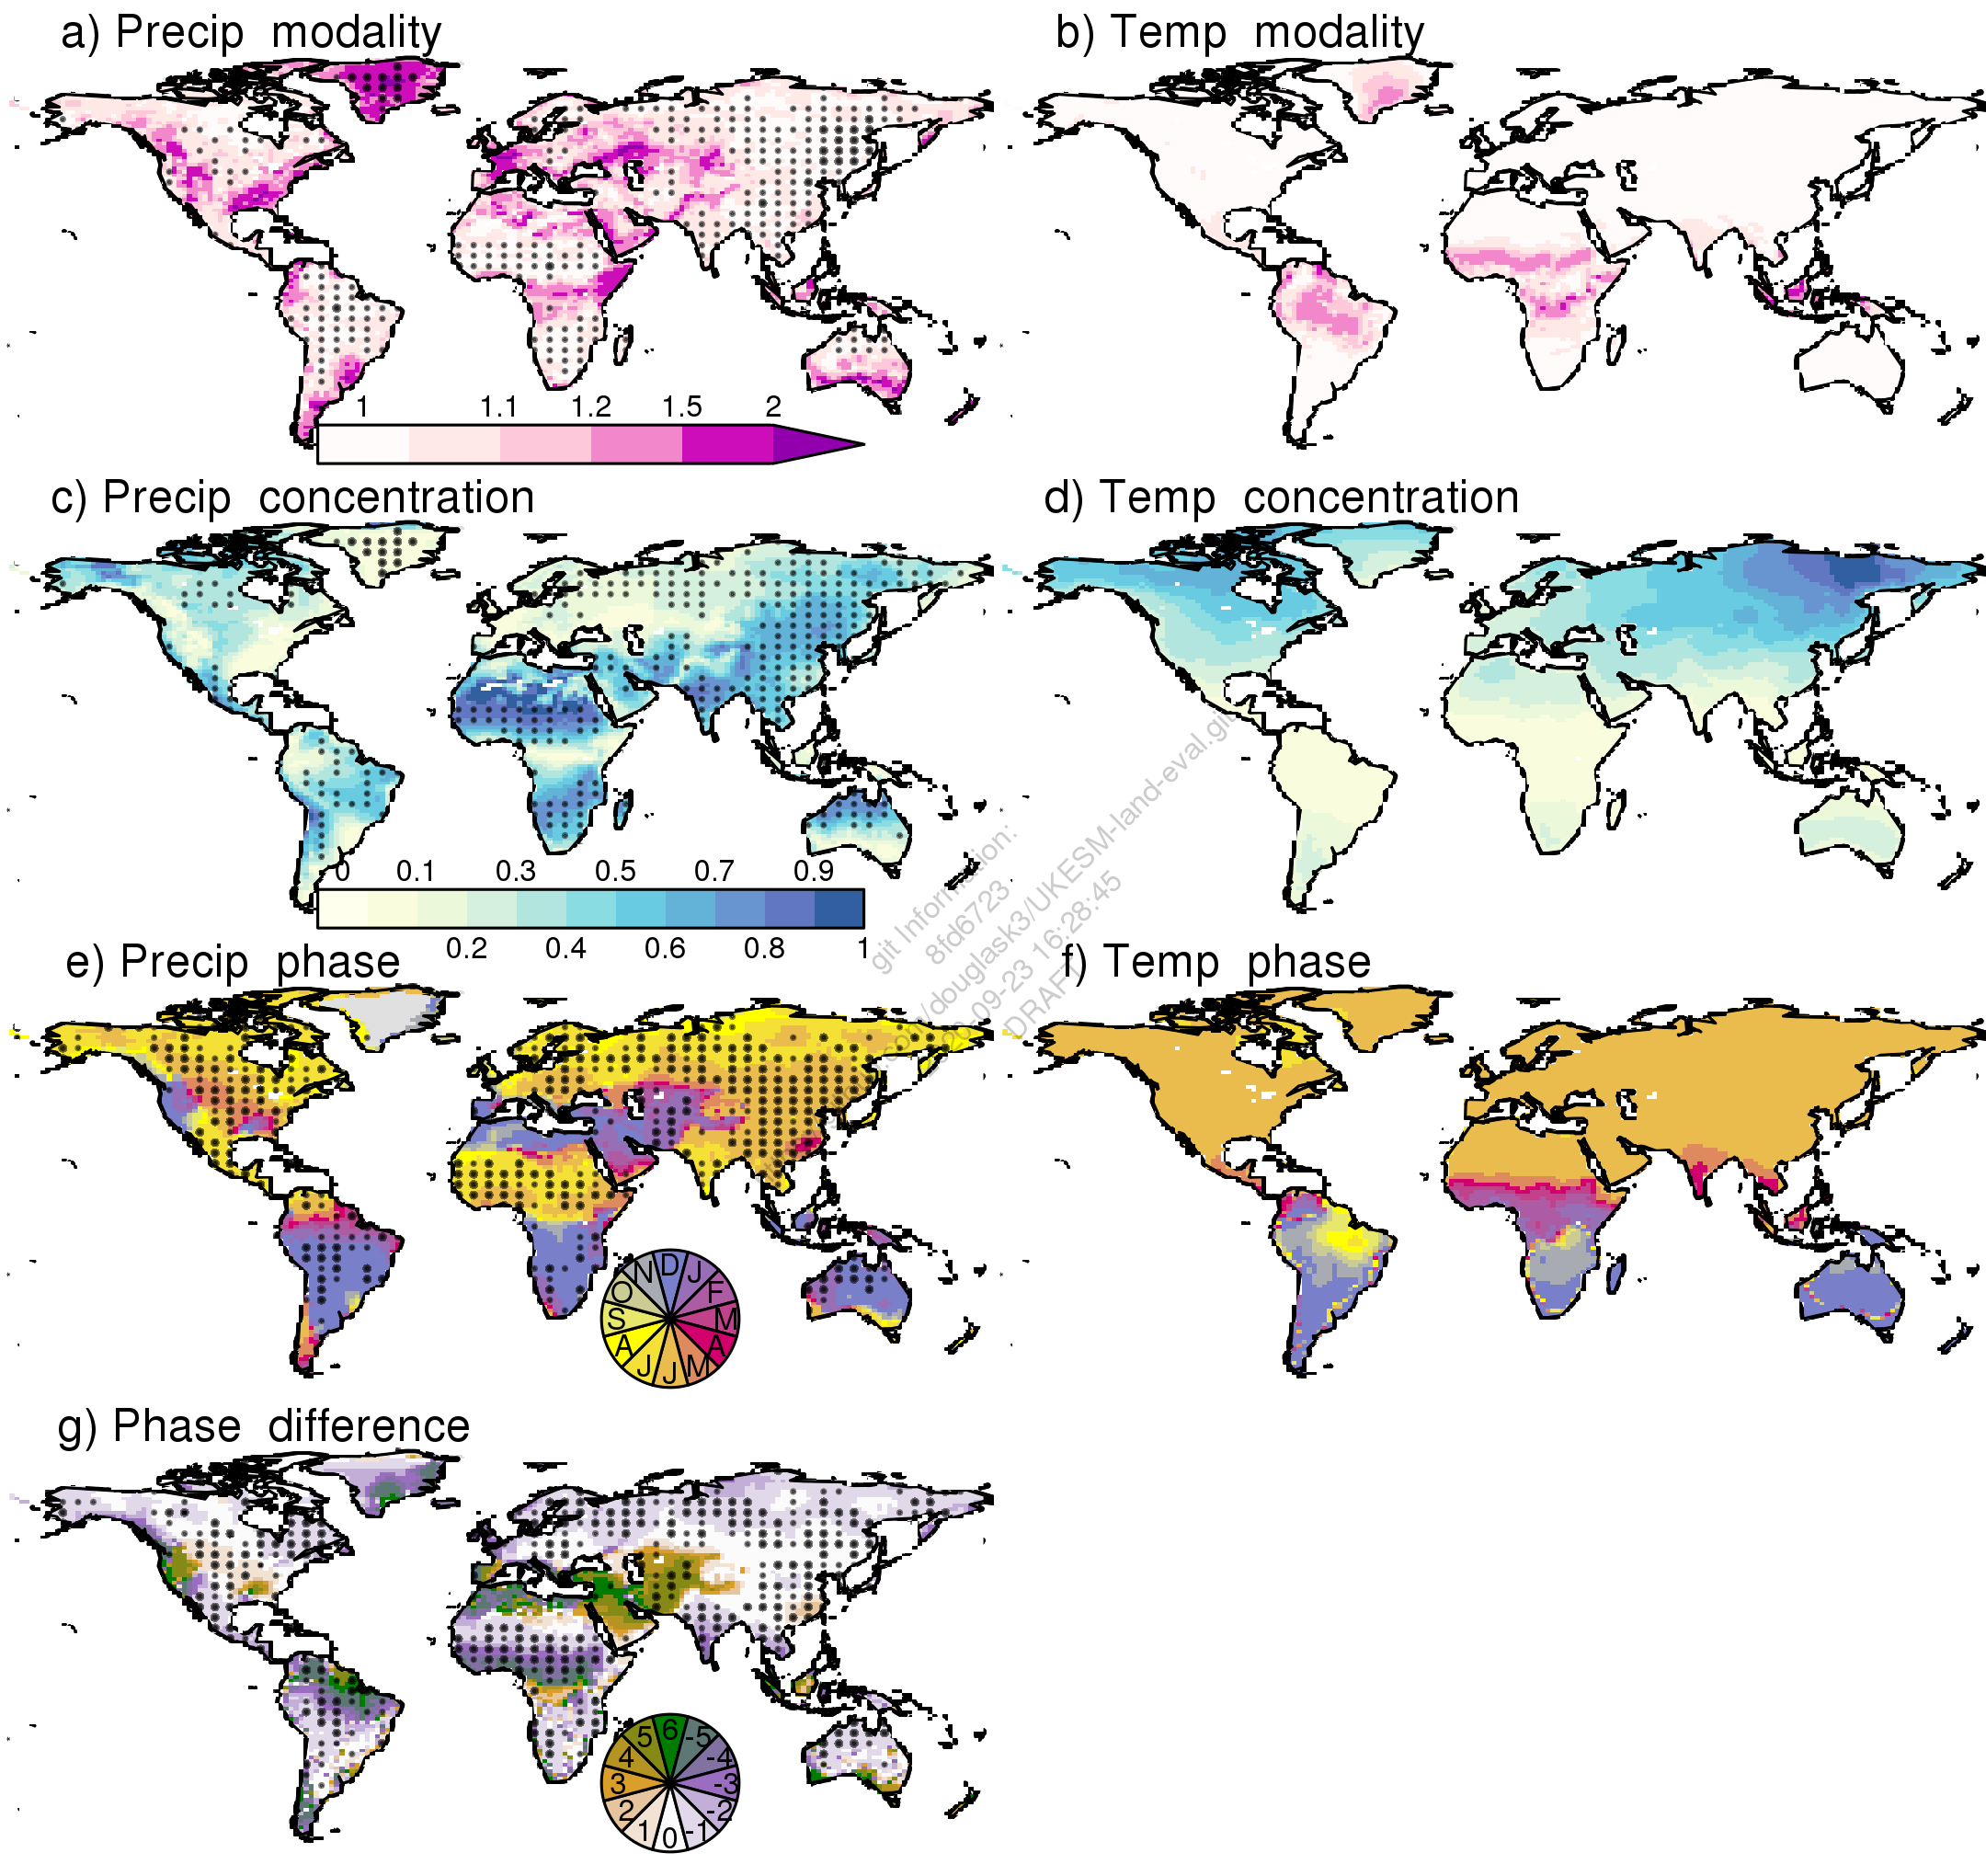
\includegraphics[width=12cm]{figs/Climate/climStuff-Observations.png}
    \caption{Observed precipitation (a, c, e) and temperature (b, d, f) seasonal metrics. a,b) modality; c,d) concentration; e,f) phase. g) shows the difference in phase between precip and temperature. Positive shows precip leading temperature, negative precip lagging temperature. Dots show smaller spread (higher confidence) across ensemble members. <<defibe>> \label{fig:ClimateSeasonObsMaps}}
\end{figure*}

\subsection{Vegetation Distribution}
UKESM reproduces the board scale vegetation distributions (Fig. \ref{fig:VegDistMap}), including high tree cover in main tropical forests and high-latitude boreal regions, some grass transition in tropical savannas and temperate grasslands, and unvegetated in major deserts and arid regions. This is reflected in a $MM$ score of xx globally. However, there are a number of biases in simulated vegetation. There is too little tree cover in the north Congo rainforest, with too rapid a transition in a southern shifted Sahel and a more extensive Sahara than seen in observations - consistent with dry, hot bias climate bias \label{fig:ClimateAAMaps}. Similarly, there is too little grass cover in areas of dry bias around the Indian monsoon. Tree cover seems to be robust against the dry bias in the Eastern Amazon. Conversely, tree cover is too extensive in South Africa, North Africa, Boreal America, SE Asia, mathcing UKESMs wet bias  \label{fig:ClimateAAMaps}. 

In many places, there the transition between arid and forested areas is too rapid \ref{fig:VegDistTri}. A lack on mix of tree and herb cover in much of the world, particularly Australia, Africa, Temperate America. The same could be true for Boreal regions, though there is disagreement in the observations here.. This can occur in the asbsence of any obsvious climate biases, such as in the Eurasian Steppe \ref{fig:VegDistTri}, which is simply partitioned between bareground and forest in the model \ref{fig:VegDistMap}. Australia and SE Asia also show to tight a transition from non-vegetated to vegetated (R2 in Fig. \ref{fig:VegDistTri})

 Too much bare soil in SE Asia, North Africa, possibly in Australia though depending on observations. 


tested with reponses in climate space

\begin{itemize}
    \item 
    \item causes too much tree cover extent and, in some places, to much bare ground with very rapid transitions (Figure  \ref{fig:VegDistMap}).
    \item grass extent is generally to small, but where grass does occur, there is too much of it.
    \item 
    \item 
\end{itemize}


\begin{figure*}[t]
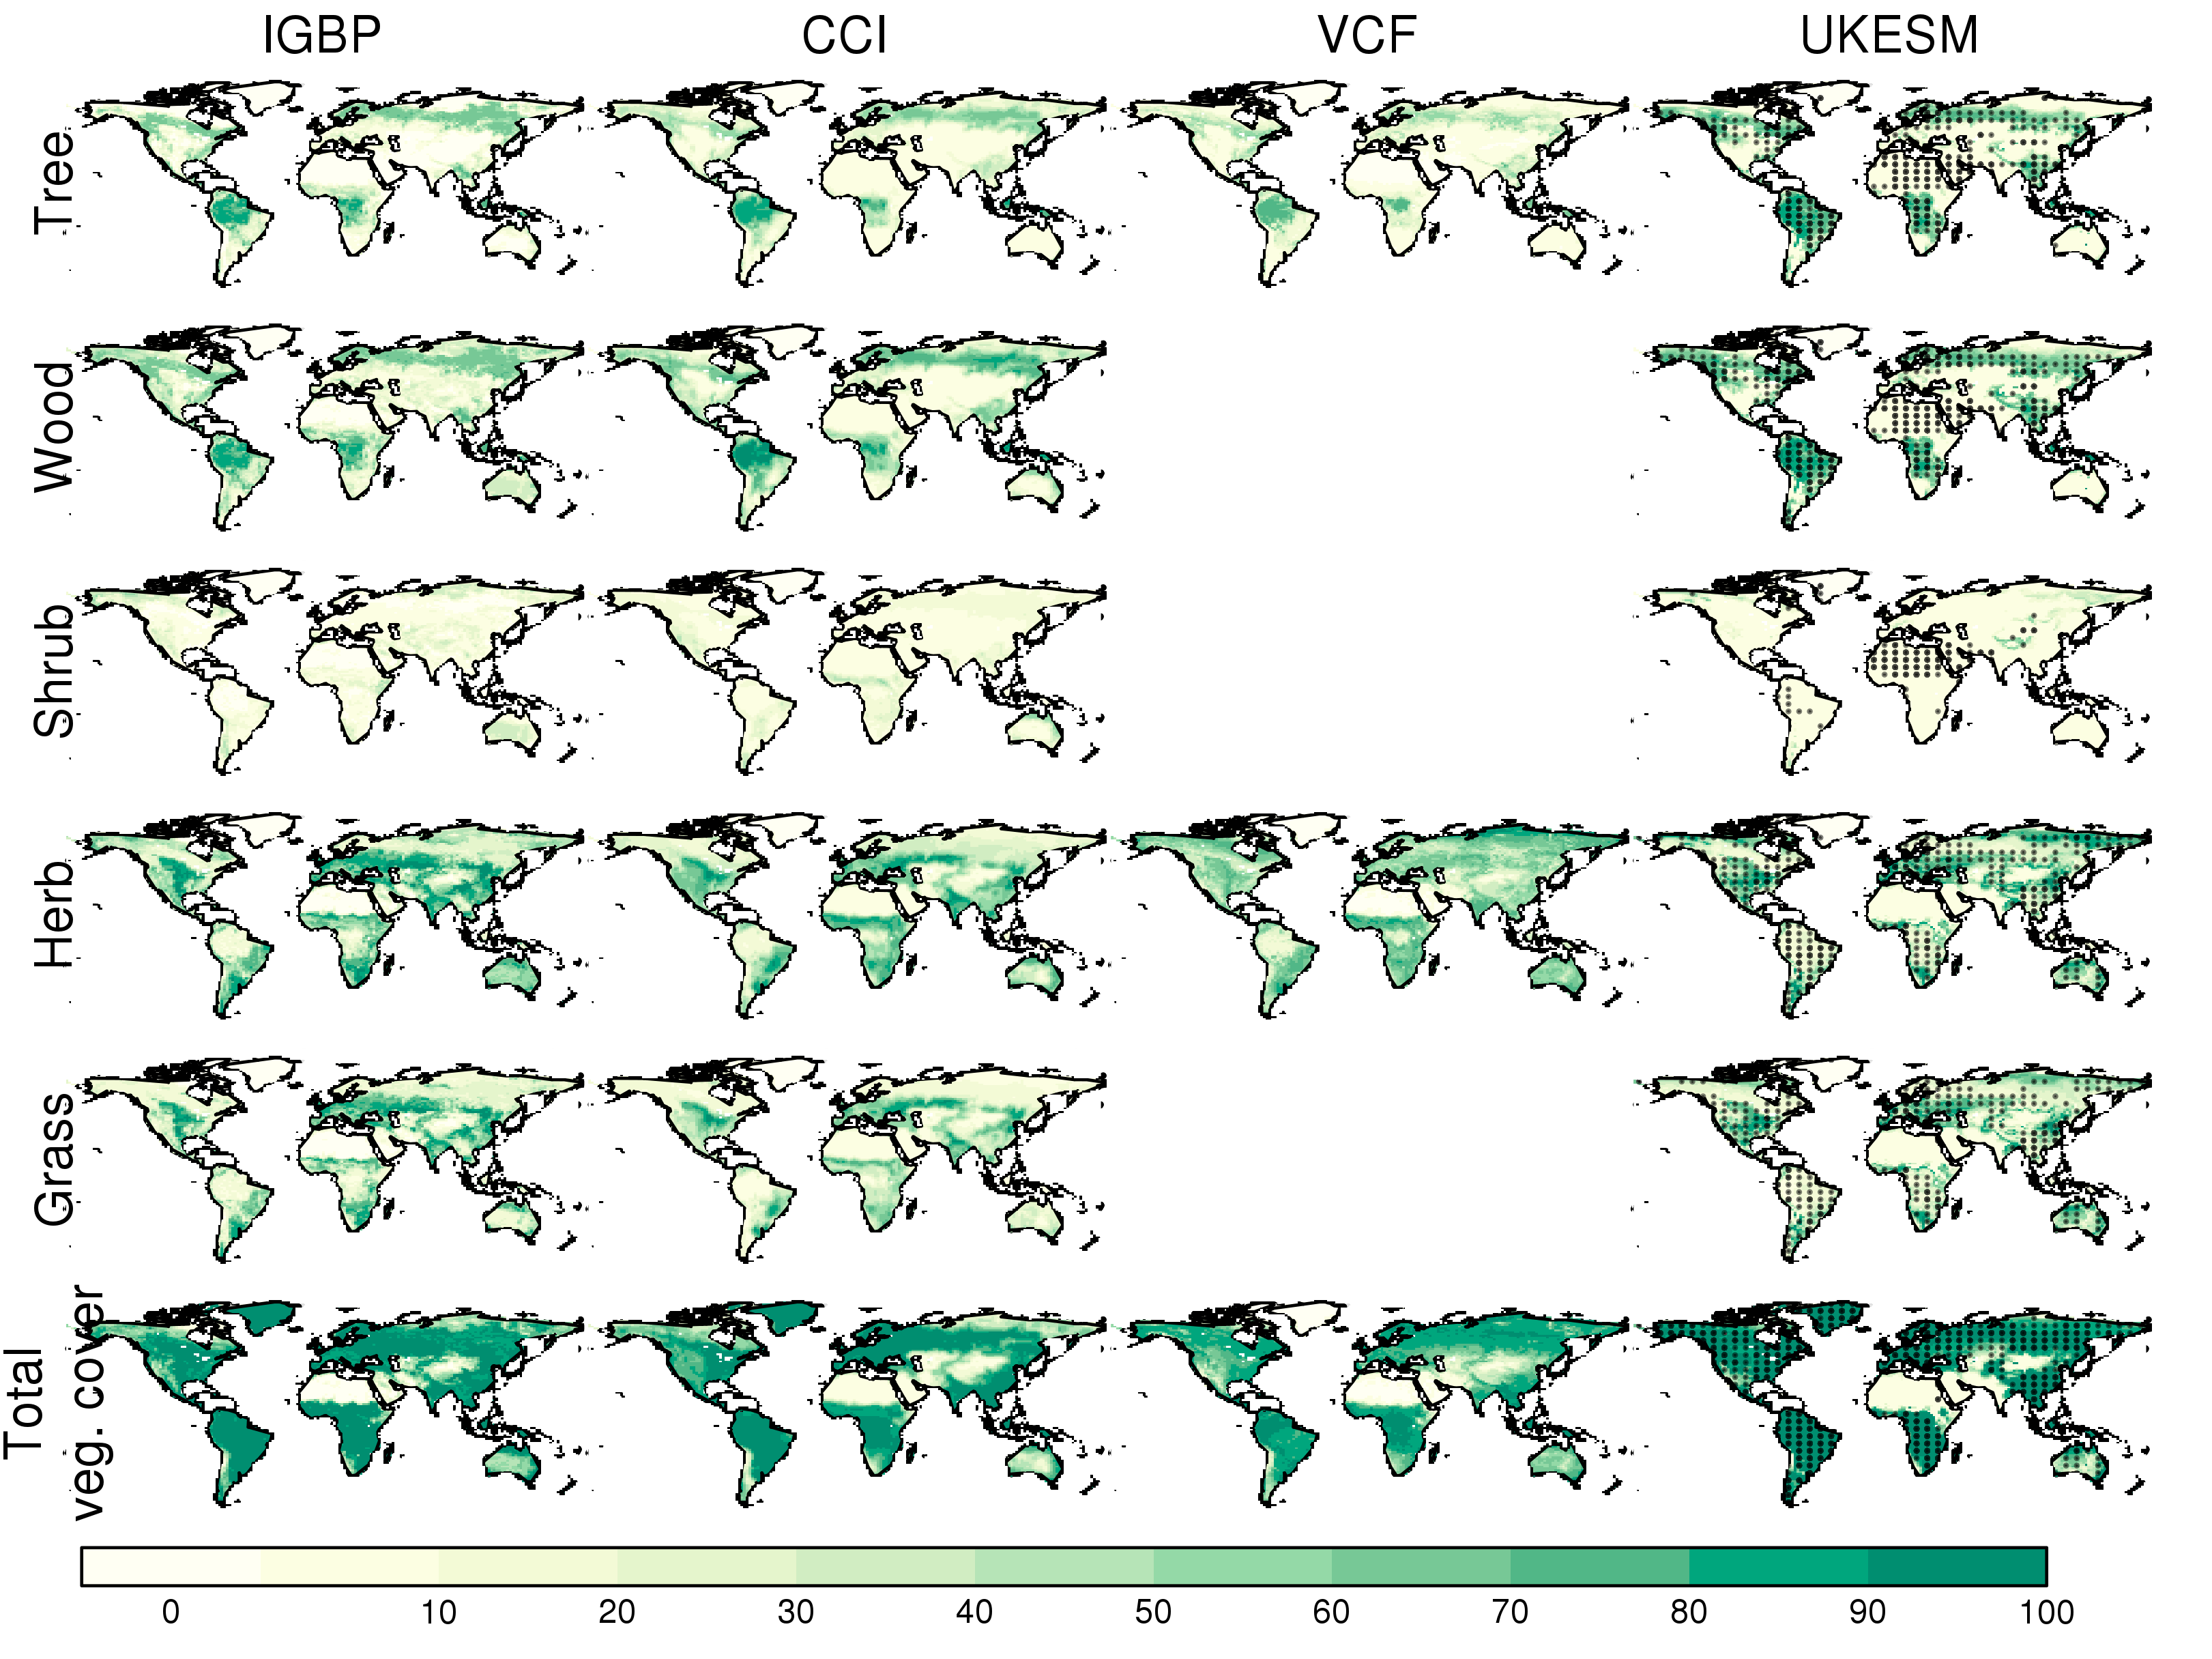
\includegraphics[width=12cm]{figs/VegDist/vegDist.png}
\caption{Observed vs simulated percentage vegetation cover. From top to bottom: Tree, wood, shrub, herb, grass and total vegetative cover. From left to right, IGBP <<ref>>, CCI <<ref>>, VCF <<ref>> observations and simulated by UKESM. Dots in the UKESM column show variation in ensemble members \label{fig:VegDistMap}}
\end{figure*}

\begin{figure}[t]
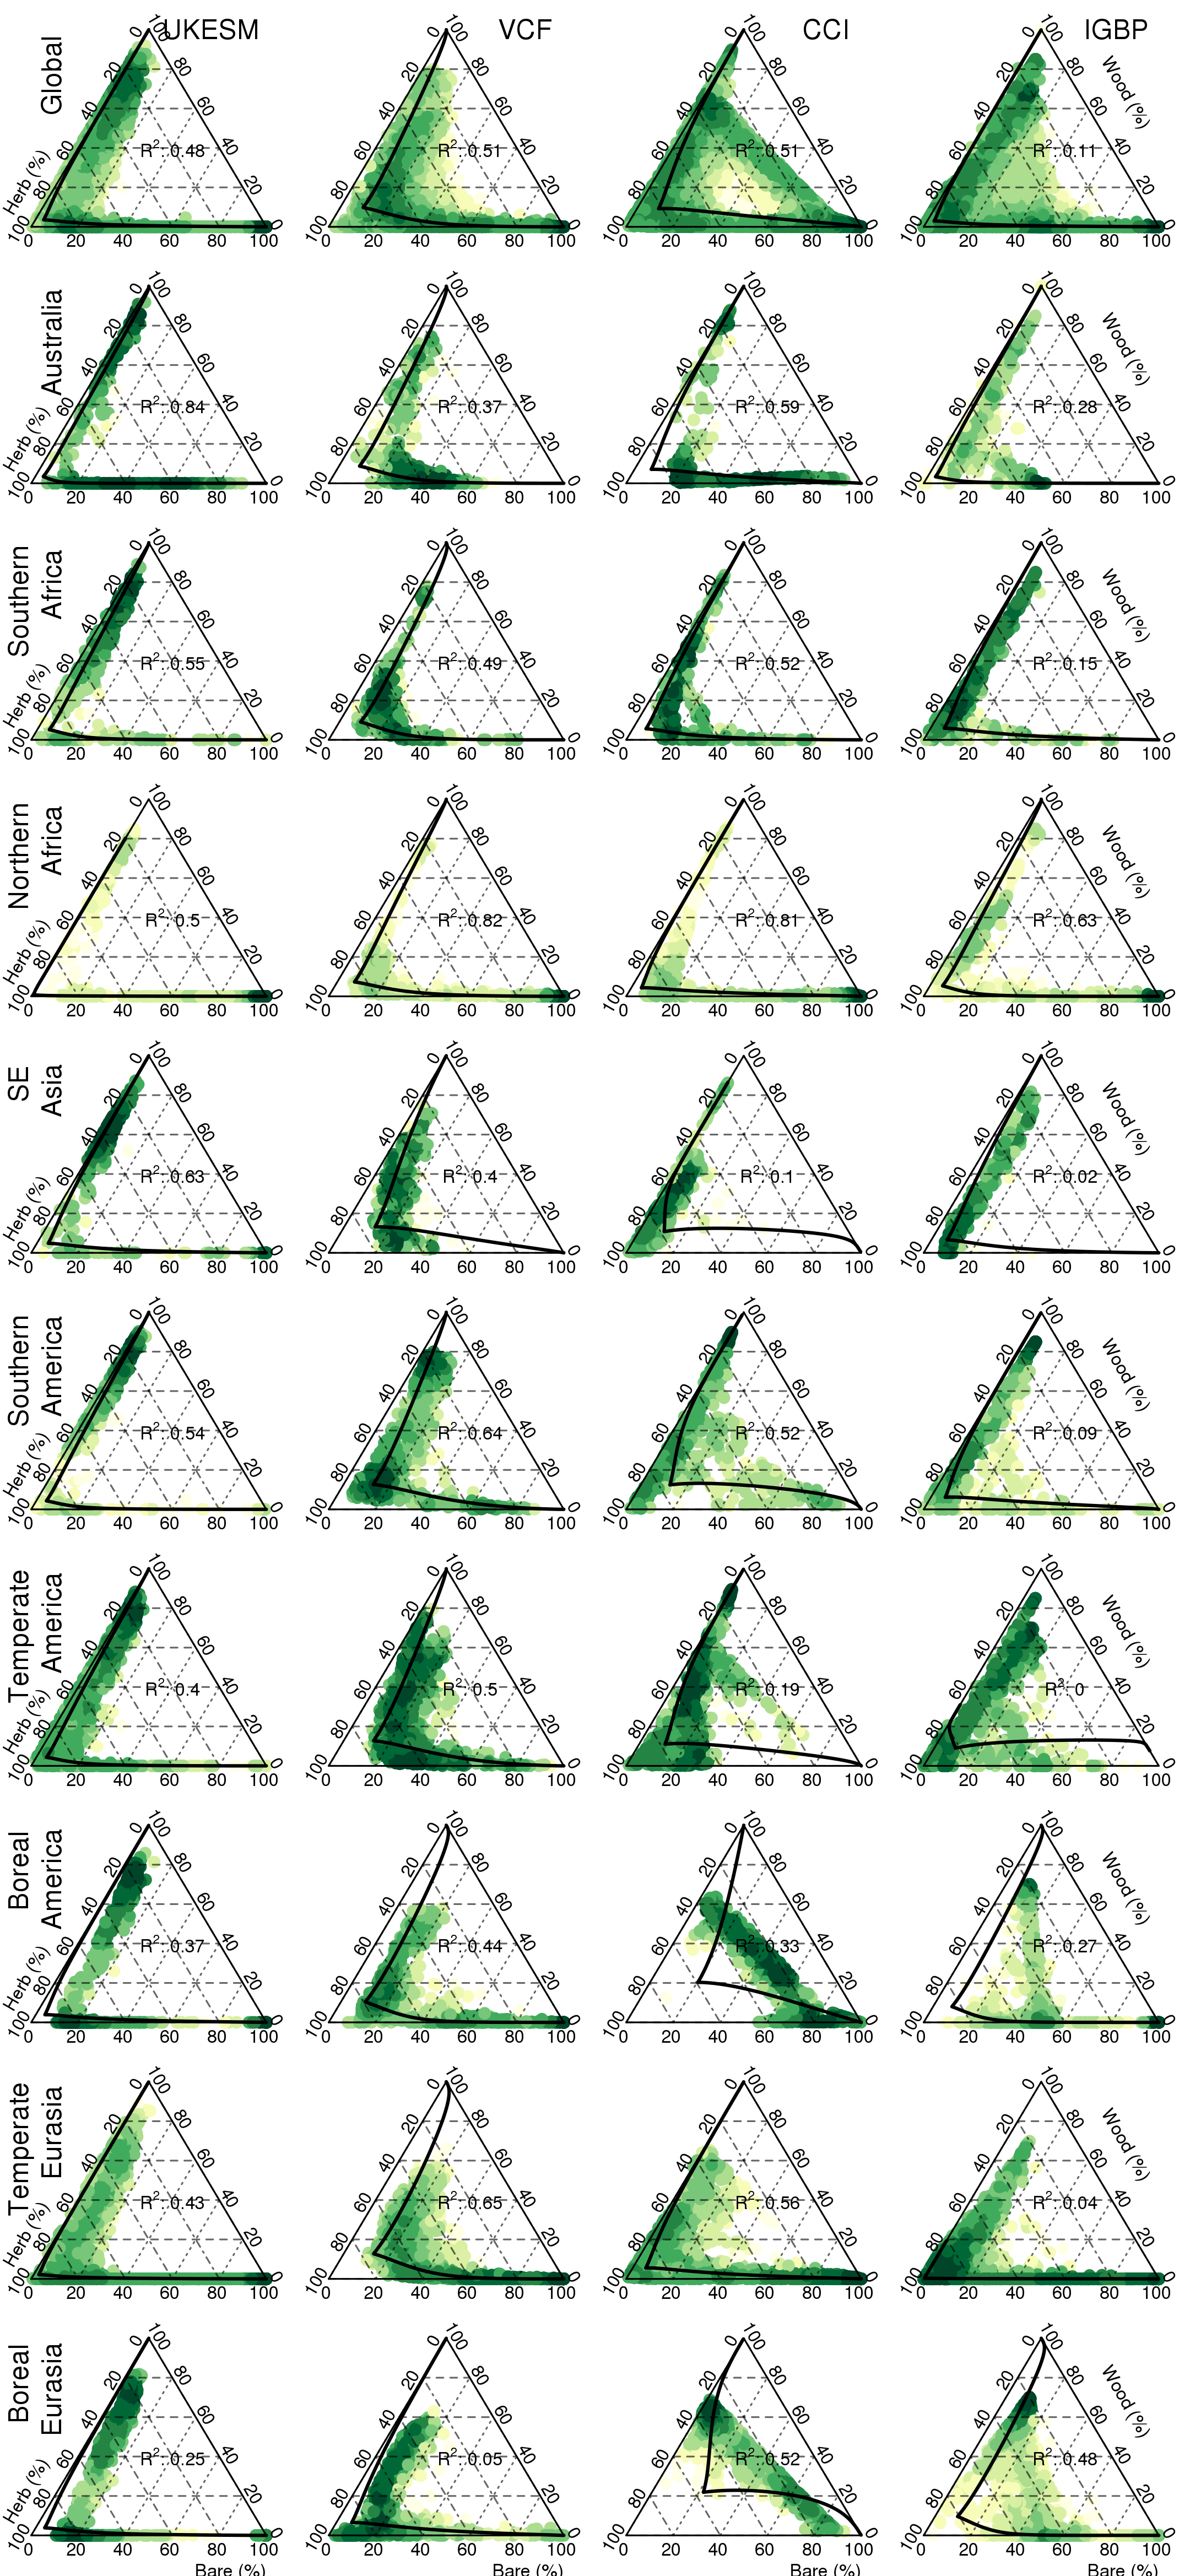
\includegraphics[width=8.3cm]{figs/VegDist/VegDistTriangle.png}
\caption{Tree (right axis), grass (left axis) and bare cover (bottom axis) variations over possible vegetated land (i.e excluding urban and water). Top row show global distributions and subsequent rows for each realm (Fig. \ref{fig:regionsMap}). First column as simulated by UKESM enemble mean, and subsequent columns for VCF, CCI, IGBP obervations <<add refs>> \label{fig:VegDistTri}}
\end{figure}

\subsection{Phenology}

\hilight{Doug - update with new LAI product}

\begin{itemize}
    \item LAI seems fine in eastern Amazon
    \item LAI is to big in Cerrado, Catinga, Miombo woodlands. Though LAI is impved  when correcting for vegtation distribution errors, though biases rmeain
\end{itemize}

\begin{figure*}[t]
    %\begin{subfigure}
        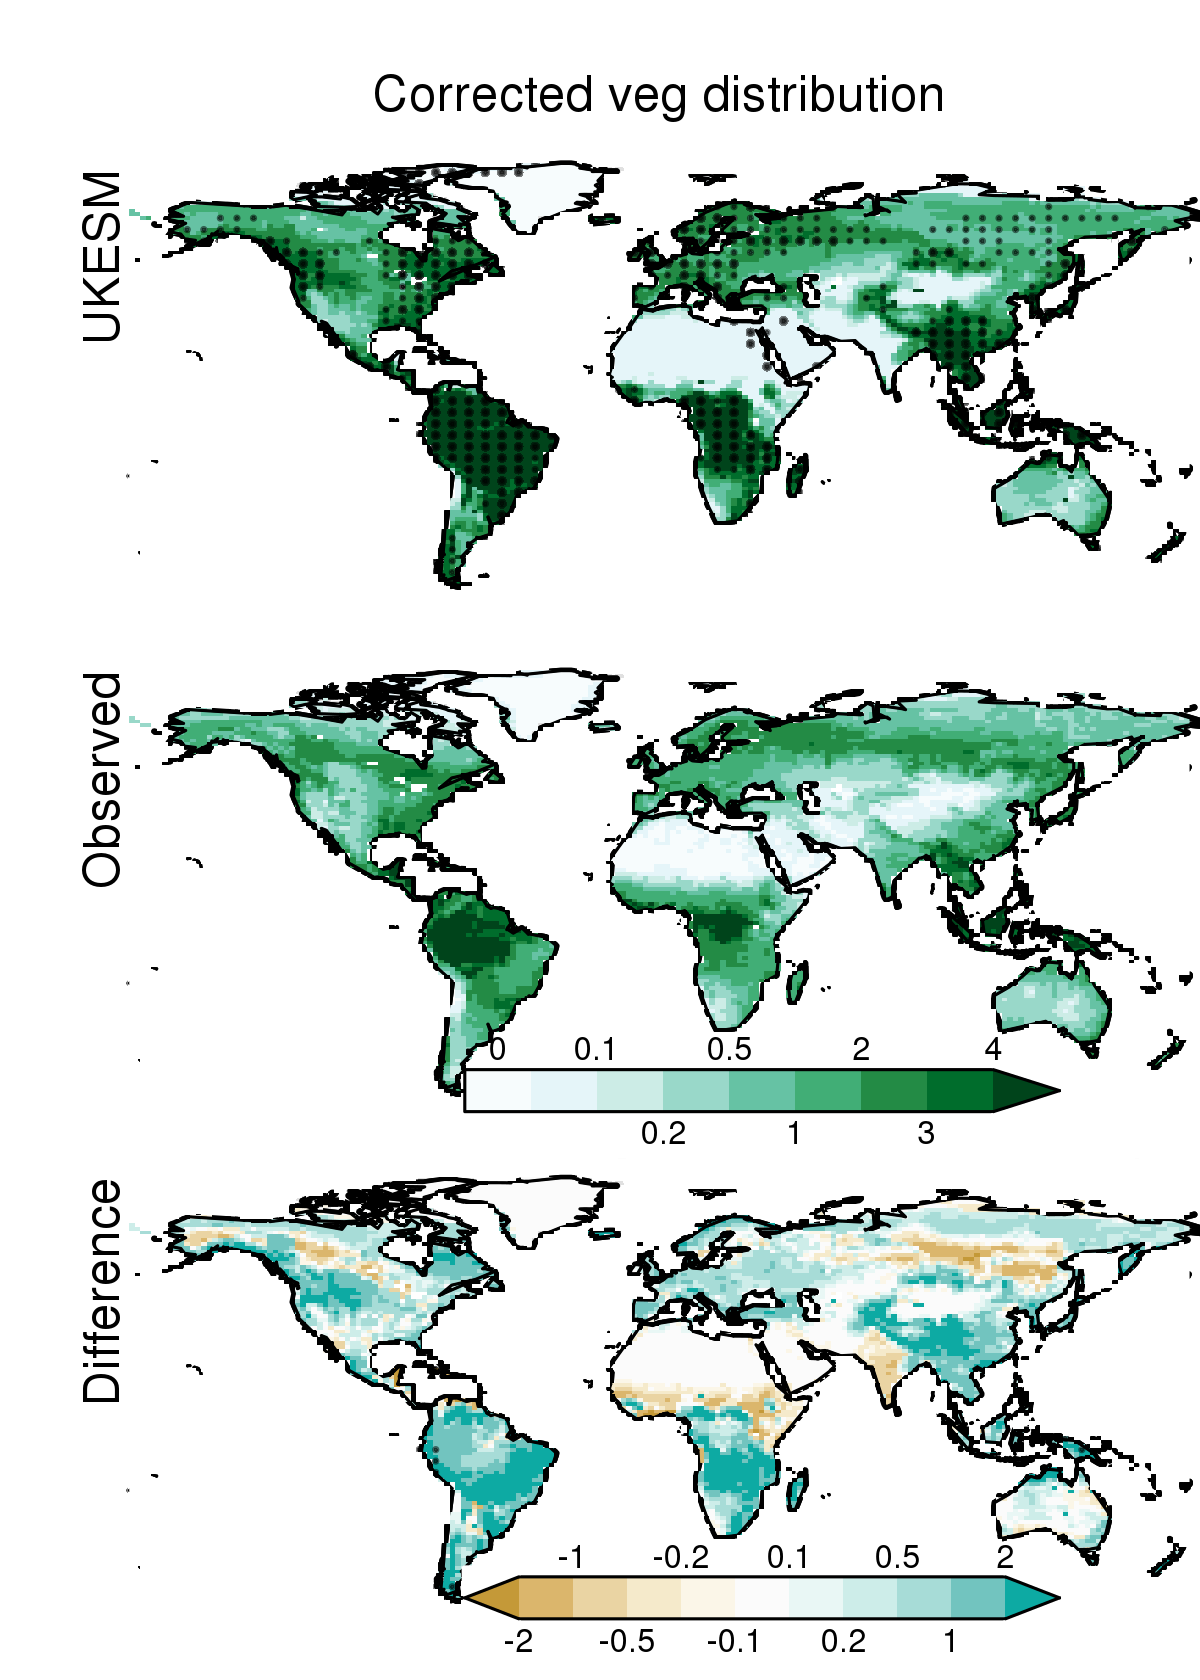
\includegraphics[width=5cm]{figs/LAI/fire_var_seasonality-maps-AA-mapscontrol-lai.png}
    %\end{subfigure}
    %\begin{subfigure}
        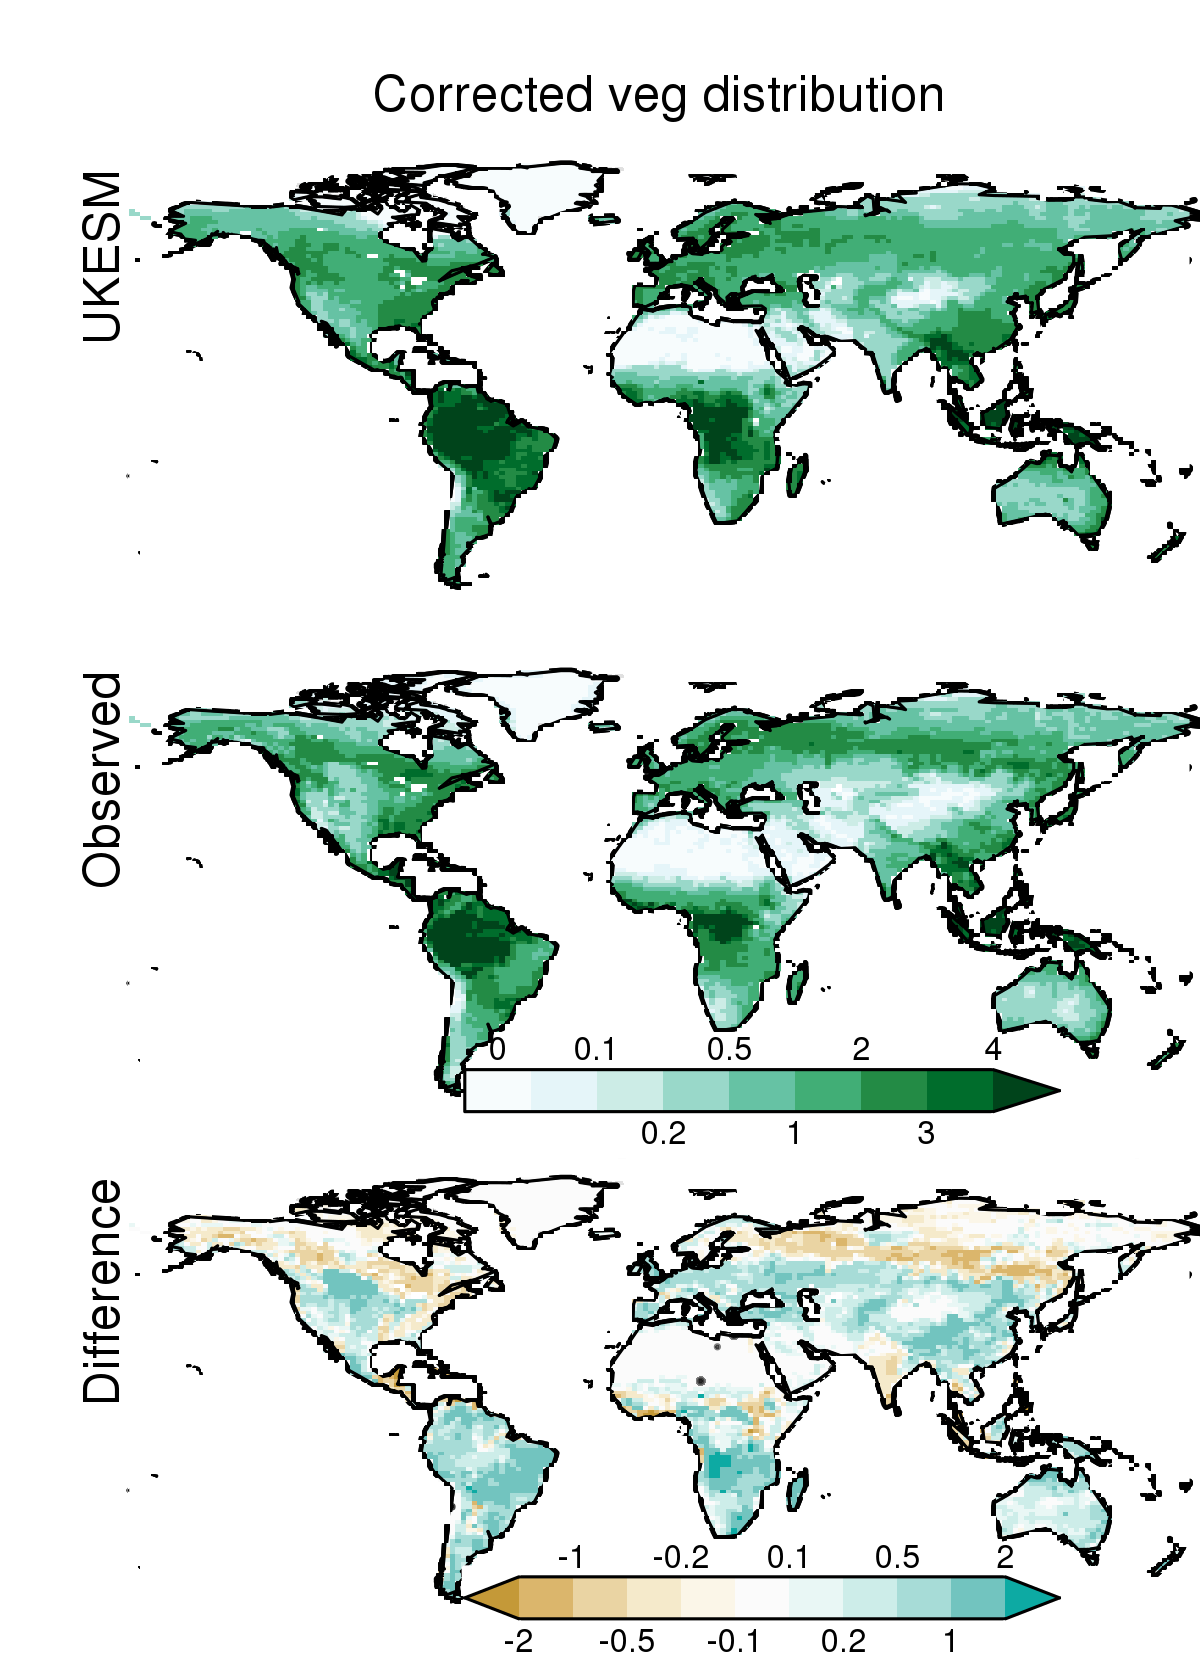
\includegraphics[width=5cm]{figs/LAI/fire_var_seasonality-maps-AA-mapsobsVegDist-lai.png}
    
    %\end{subfigure}
    \caption{Simulated (top), observed (middle, <<ref>>) and different in mean annual LAI for 2001-2013. Right hand, UKESM has been corrected for vegetation distribution biases \label{fig:LAImap}}
\end{figure*}

\begin{figure*}[t]
    %\begin{subfigure}
        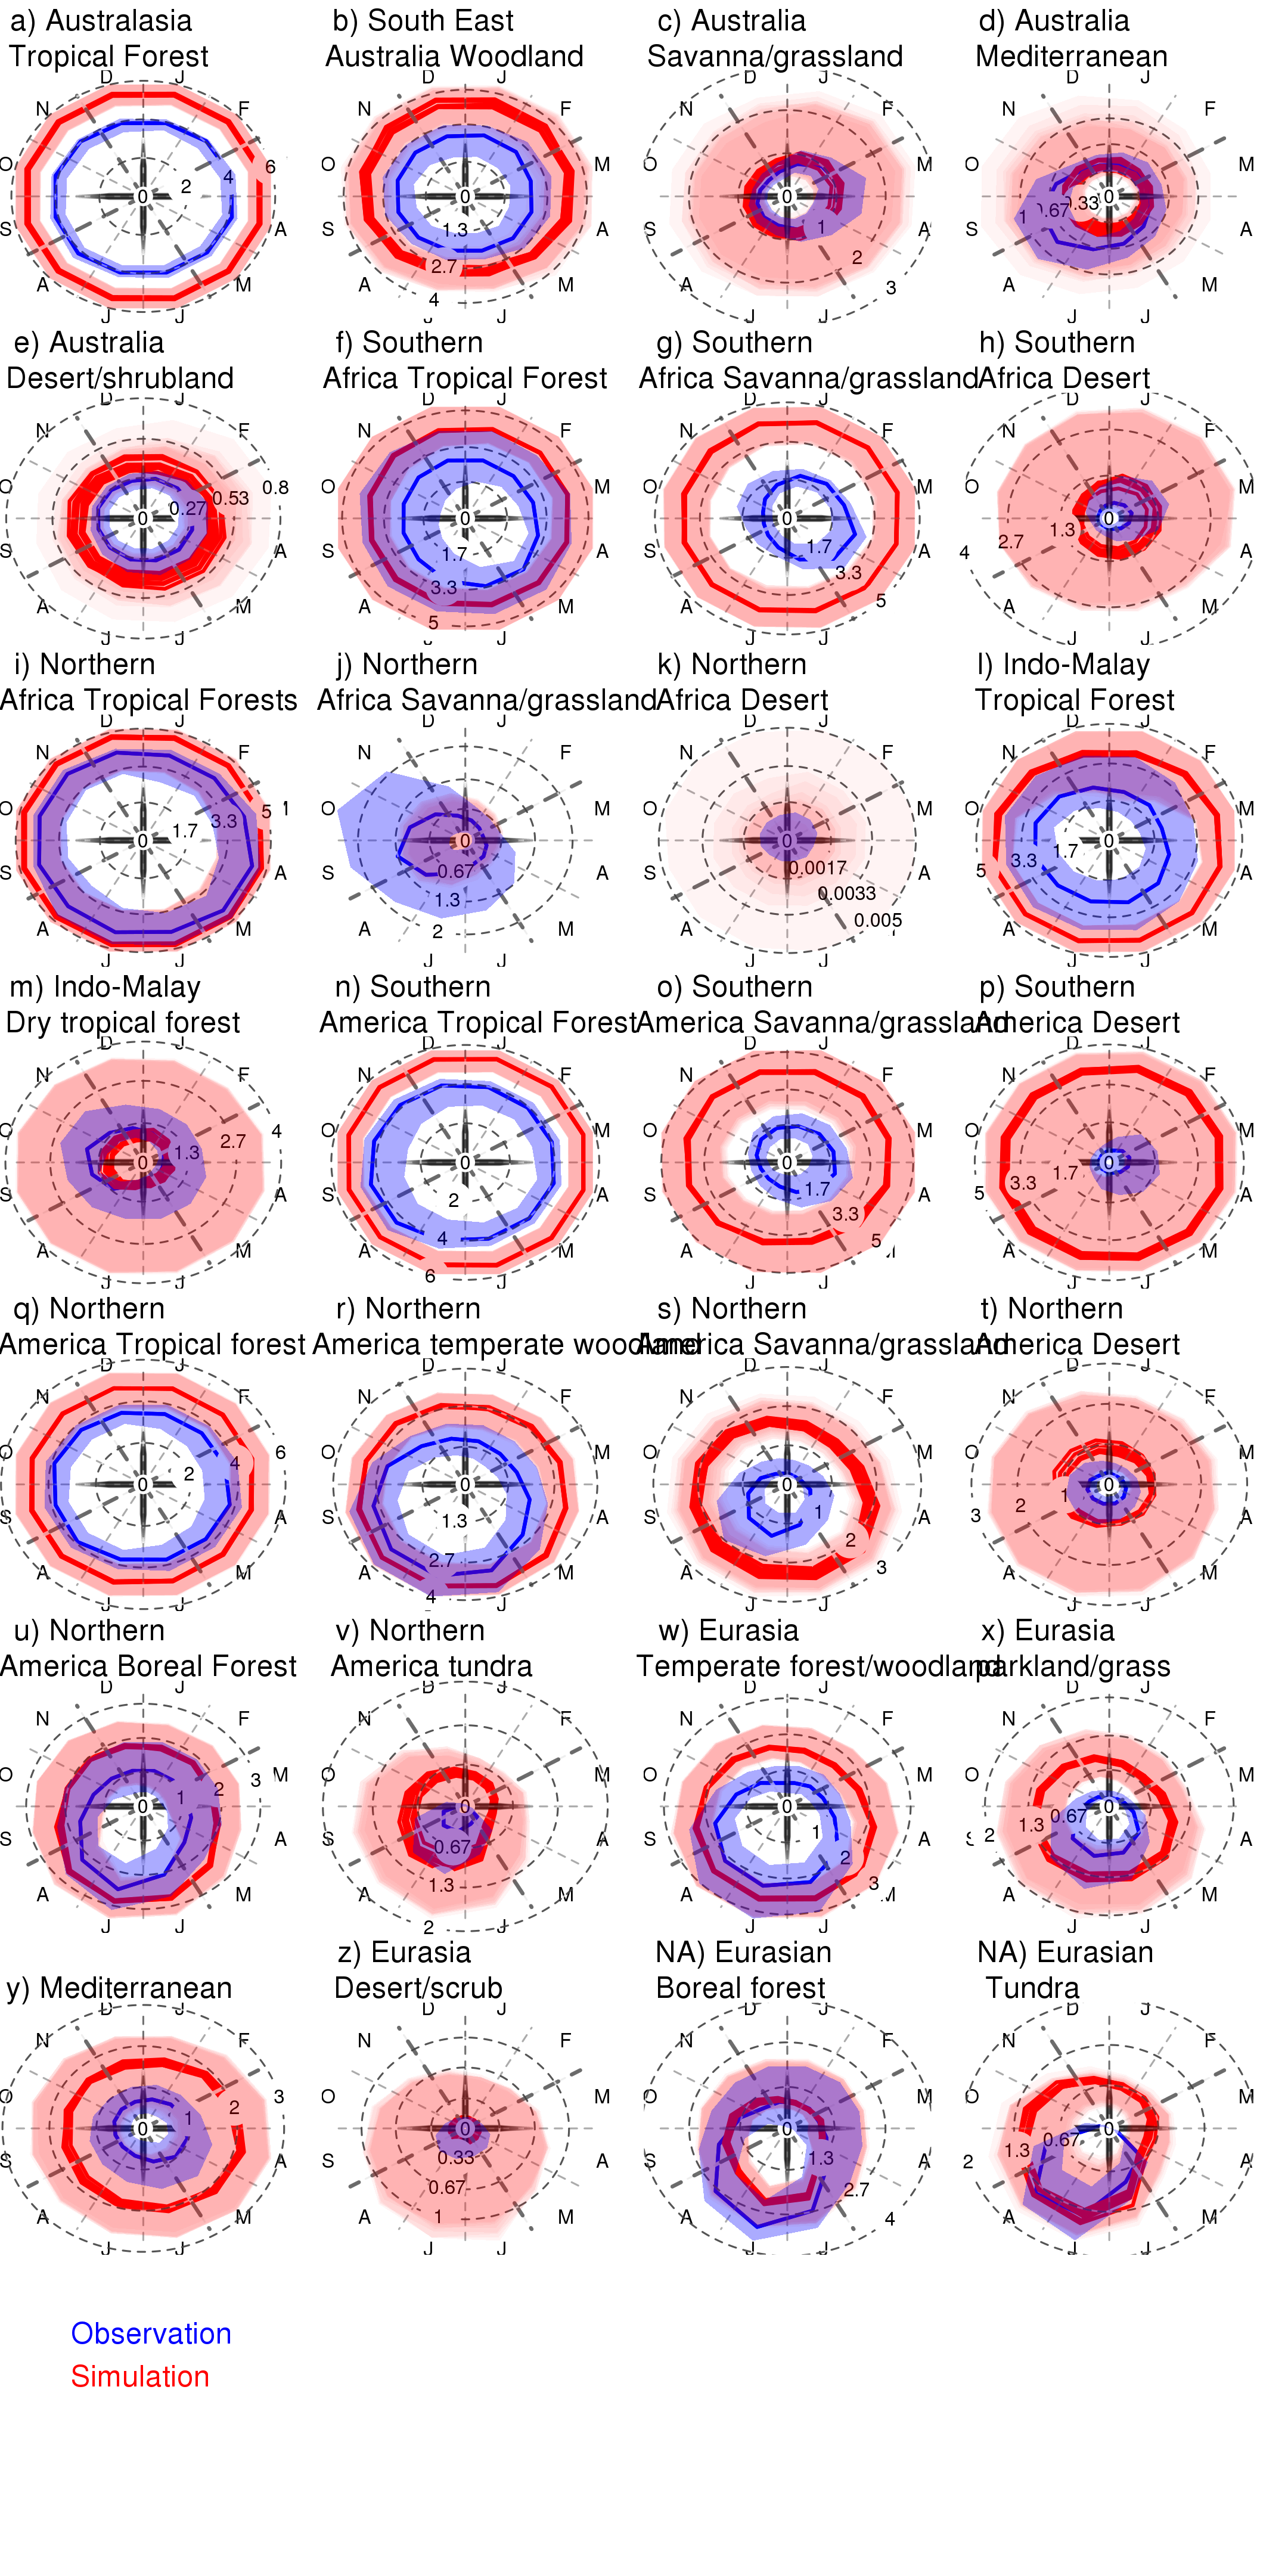
\includegraphics[width=5cm]{figs/LAI/fire_var_seasonality-TS-control-lai.png}
    %\end{subfigure}
    %\begin{subfigure}
        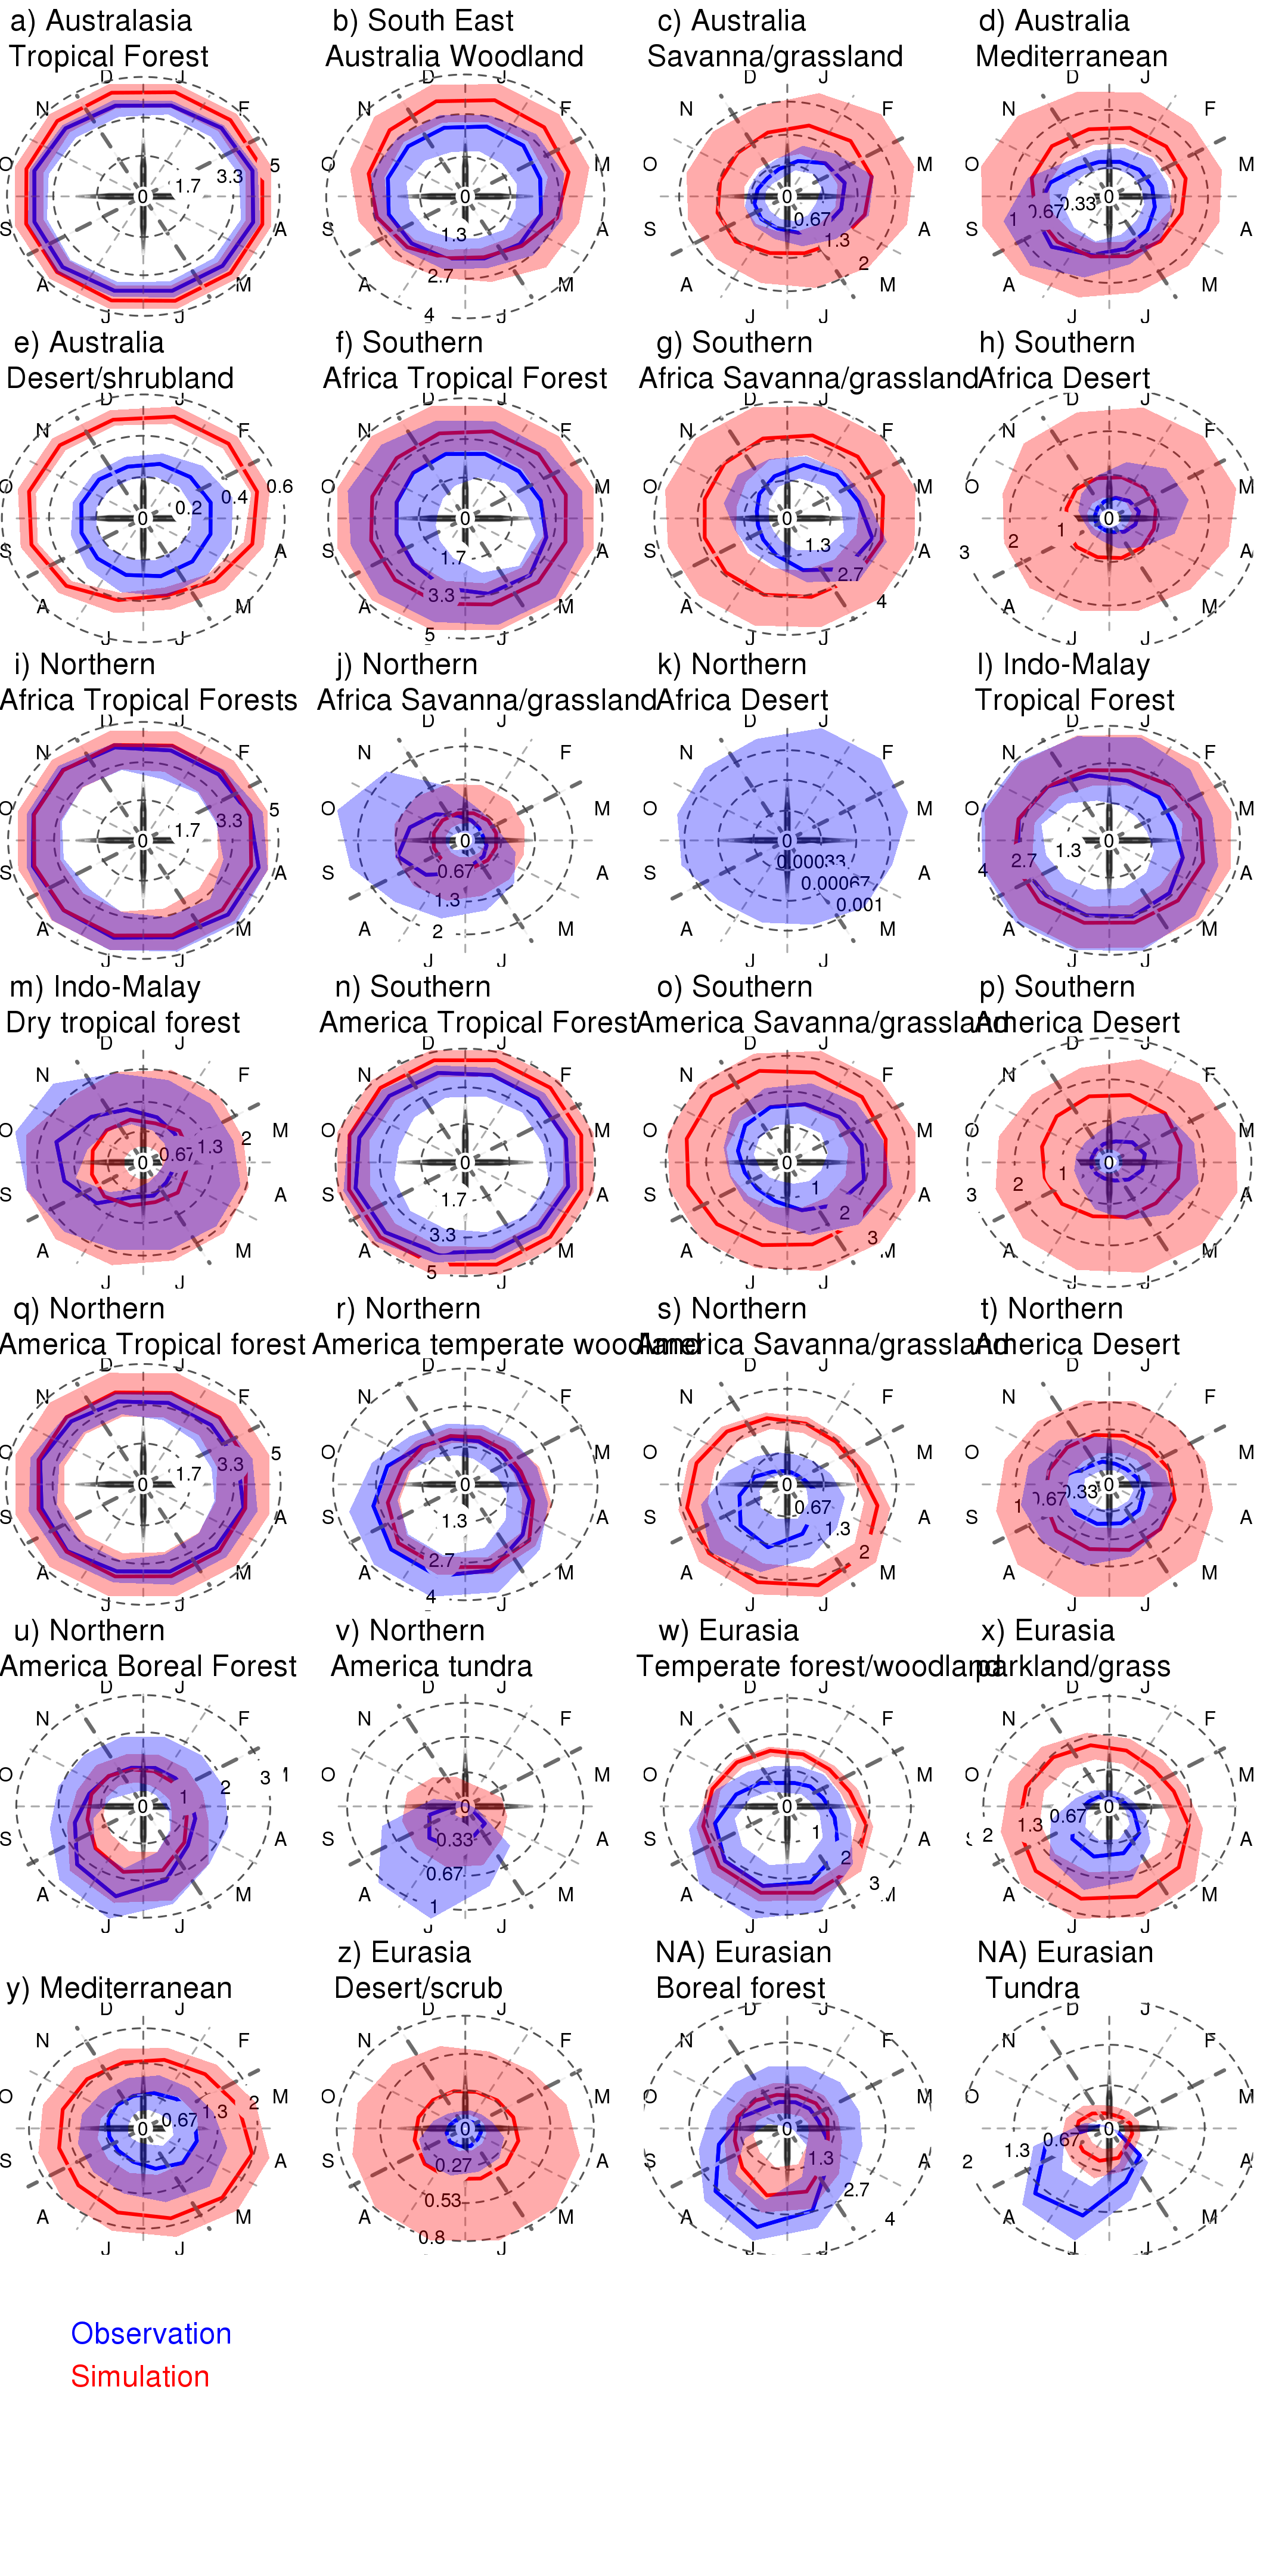
\includegraphics[width=5cm]{figs/LAI/fire_var_seasonality-TS-obsVegDist-lai.png}
    
    %\end{subfigure}
    \caption{Simulated (red), observed (blue, <<ref>>) and seasonal cycles in LAI for 2001-2013 for each region(see \ref{fig:regionsMap}. Right hand, UKESM has been corrected for vegetation distribution biases \label{fig:LAIseasonalTS}}
\end{figure*}

\begin{figure*}[t]
    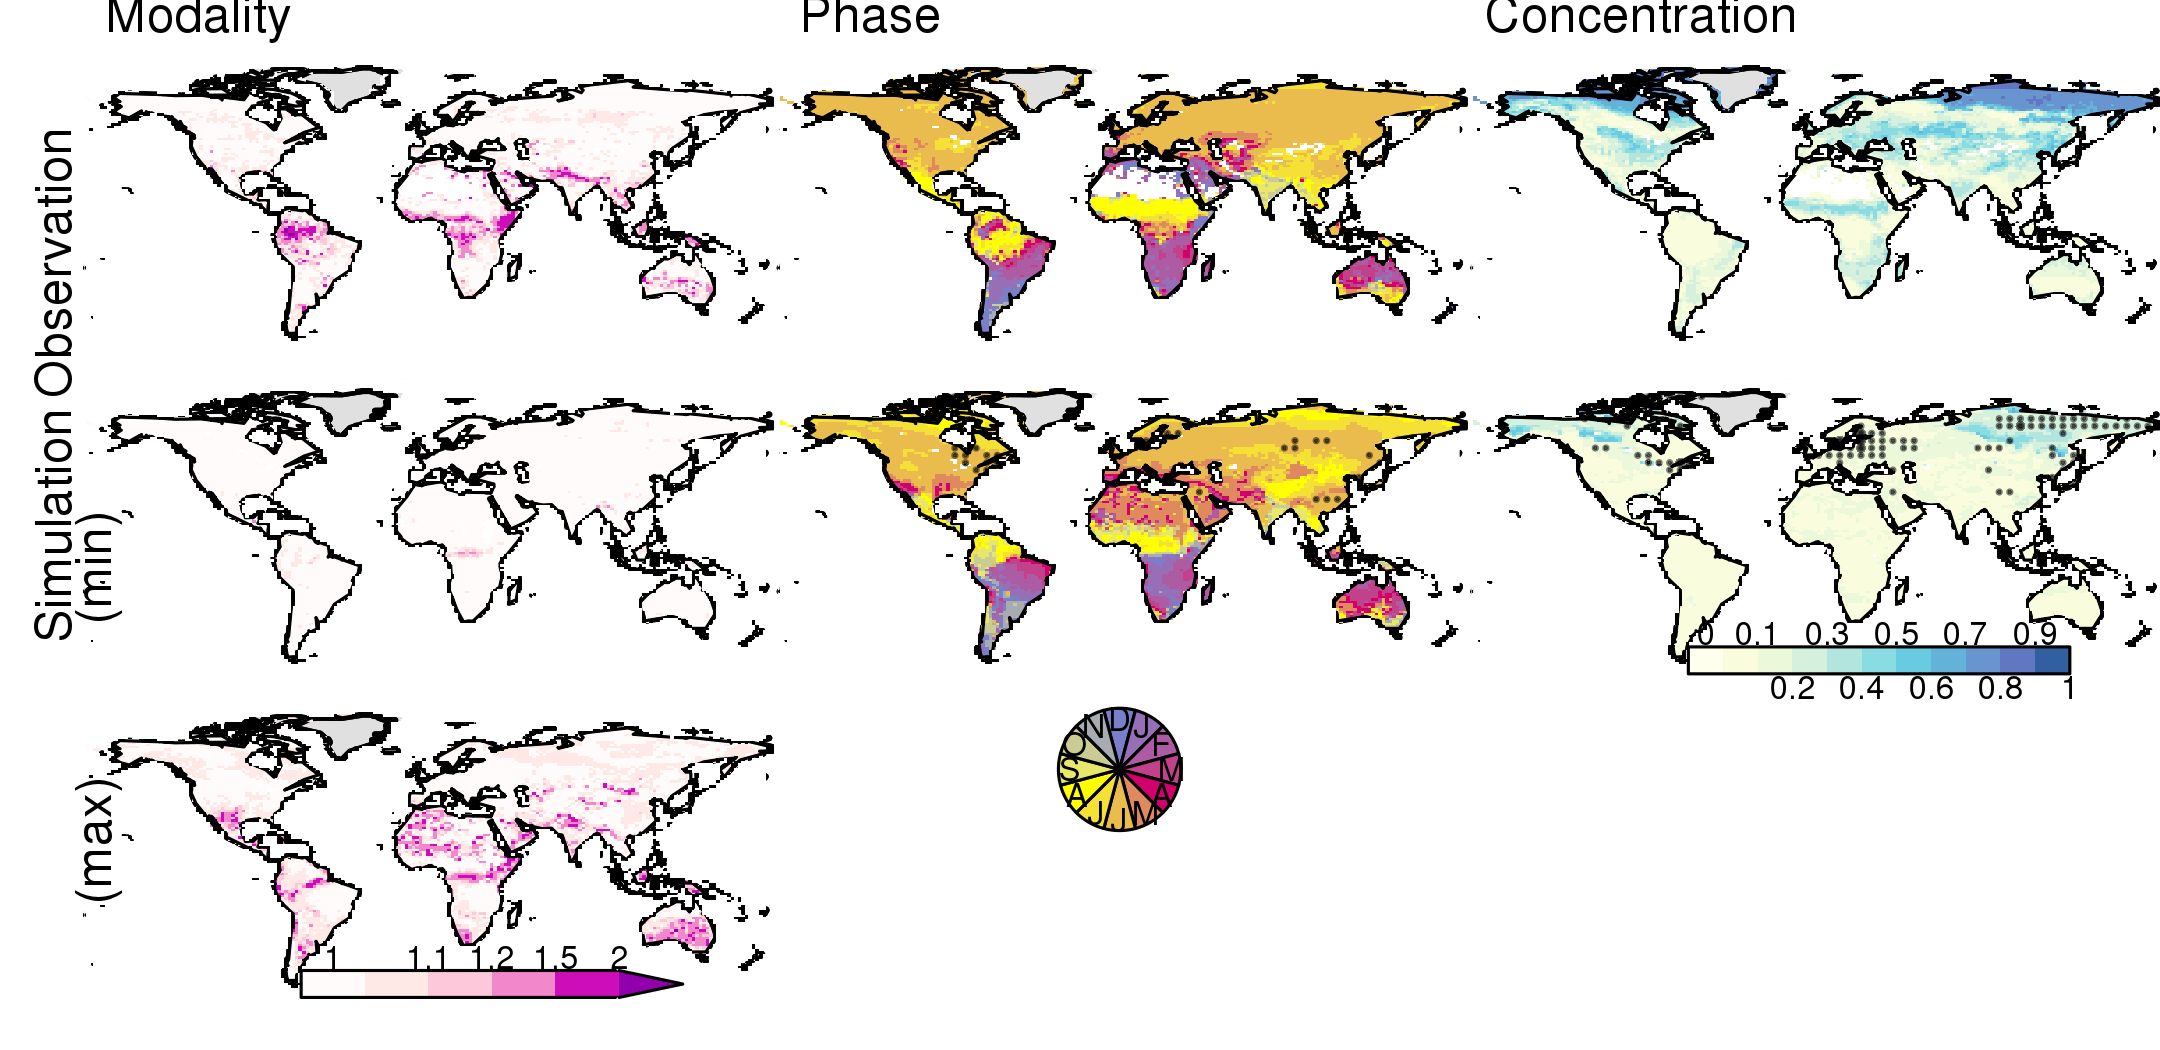
\includegraphics[width=12cm]{figs/LAI/fire_var_seasonality-maps-MPCcontrol-lai.png}
    \caption{Seasonal comparison for LAI \label{fig:LAIseasonalMap}}
\end{figure*}

\subsection{Carbon}
\hilight{Eddy - include fluxnet?}

\begin{itemize}
    \item Site-mean seasonal peak is not prolonged enough, dropping off too quickly in Jul-Sept. Seems to be an error in US sites.
    \item Spatial distribution of GPP is good. Too little in some tropical regions (inc. India), possibly related to climate (precip.) biases? To much in other tropical regions. Plots show obs, model, bias
    \item \hilight{Doug - remember to add veg distribution biases}
\end{itemize}

\subsubsection{Vegetation carbon}

\begin{itemize}
    \item lack of grass and tree cover in Sahael and India lead to less production than seen in obervations (Fig.). 
    \item Despite maintaining high tree cover, the dry bias in the Eastern Amazon also caused a lack of prioduction and veg carbon
    \item lack of productivity in Eurasian Steppe.
\end{itemize}
\hilight{Eddy/Chantelle. Anything in iLamb?}
\hilight{Doug - use fireMIP stuff}

\subsubsection{Soil carbon}
\hilight{Eddy/Chantelle. Anything in iLamb?}

\subsection{Soil moisture}
%\hilight{Ranjini?} 
%this is in here for HadGEM3 - %https://agupubs.onlinelibrary.wiley.com/doi/full/10.1029/2018MS001370
\hilight{Doug: Soil moisture in climate space}

\subsubsection{Cold processes including albedo}
\hilight{Eleanor - we need to decide what is different between JULEs-ES and GL7 - I suspect we actually need only an albedo plot}
%\hilight{Eleanor - bit of text & can I get original figures (they didnt copy into google docs vert well)}
\hilight{Rob P - want to make a plot?}

\subsubsection{LST}
\hilight{Rob K}

\subsubsection{Drought}
\hilight{Phil - bit of a summary of results}
\begin{figure*}[t]
    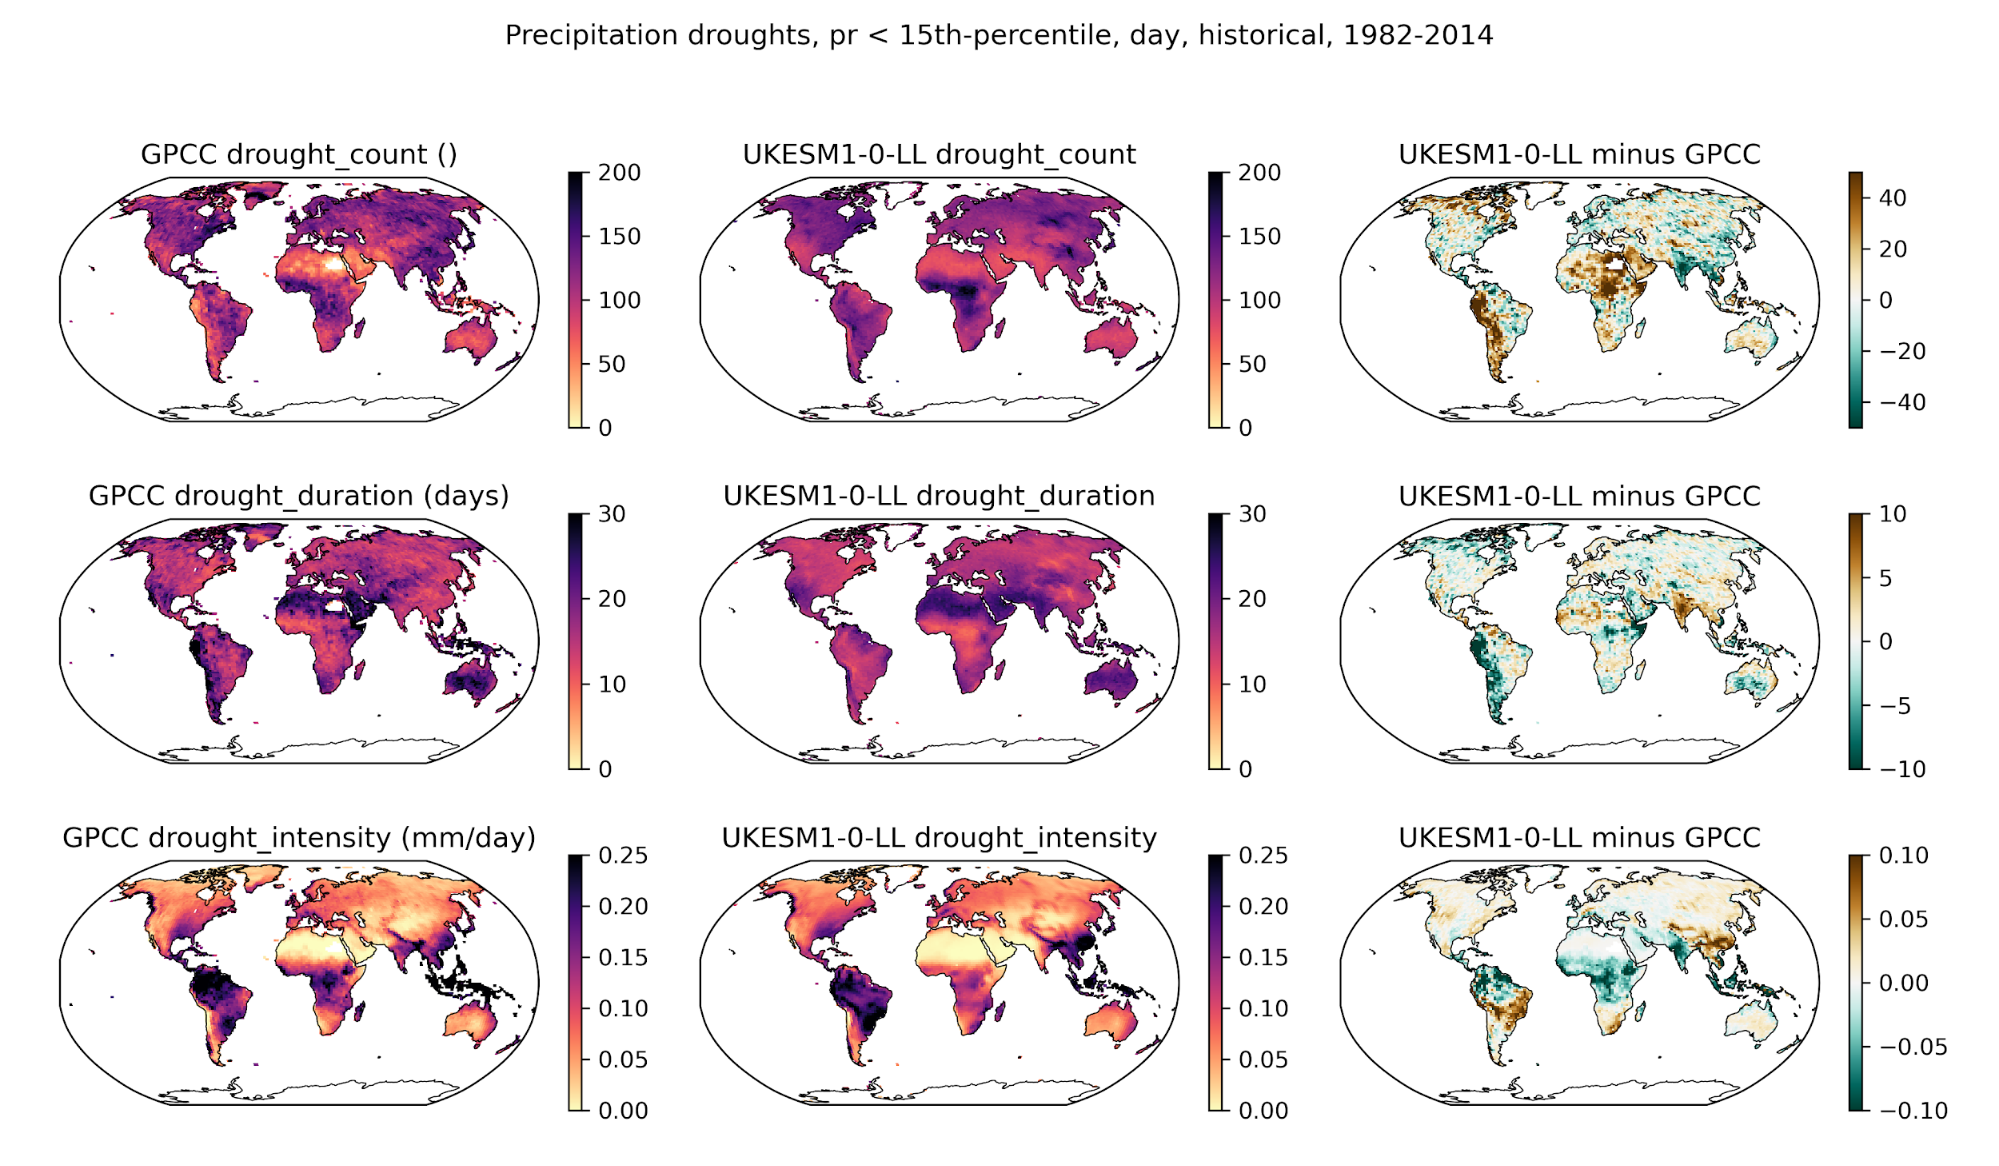
\includegraphics[width=6cm]{figs/drought.png}
    \caption{Caption Phil? \label{fig:drought} }
\end{figure*}




\hilight{Rebecca - I would if we could also do a veg fraction "turnover"?}






\subsubsection{GPP}
\begin{itemize}
    \item Too little in some tropical regions (inc. India), possibly related to climate (precip.) biases? To much in other tropical regions. Plots show obs, model, bias.
\end{itemize}

\begin{figure*}[t]
    %\begin{subfigure}
        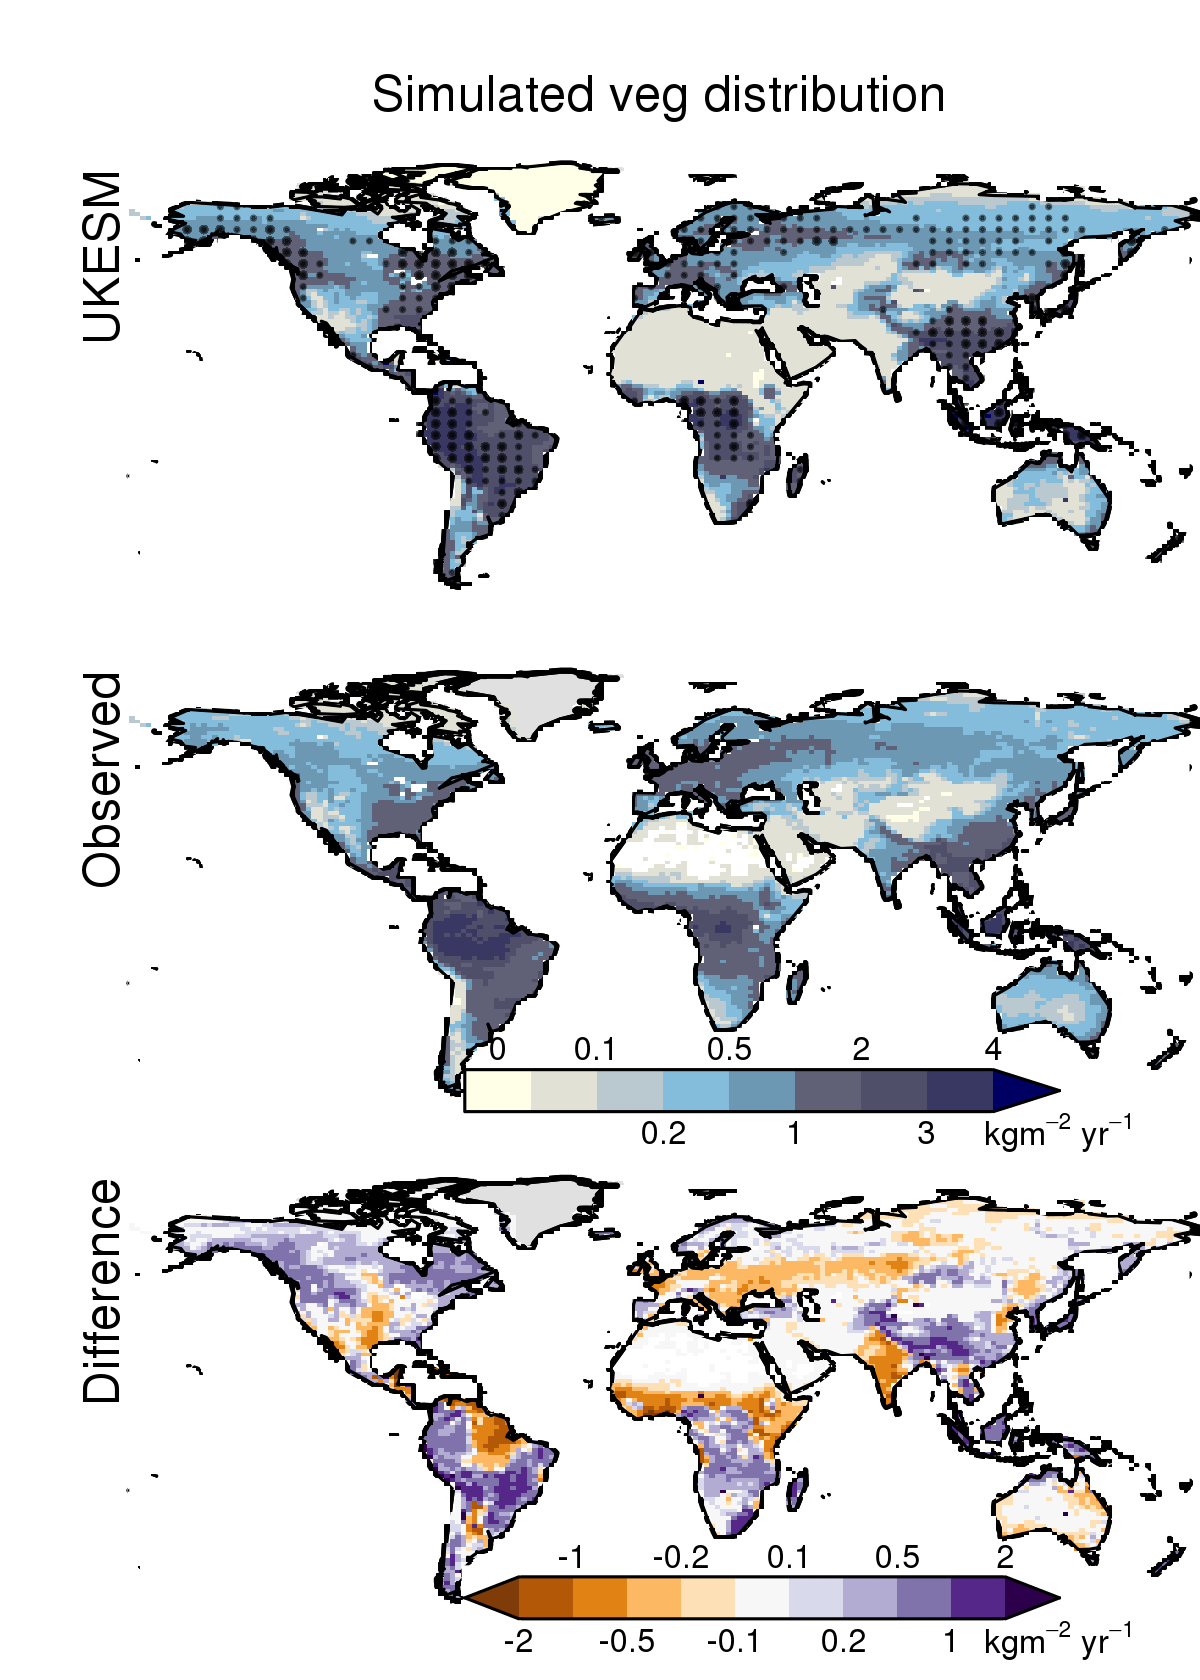
\includegraphics[width=5cm]{figs/GPP/fire_var_seasonality-maps-AA-mapscontrol-gpp.png}
    %\end{subfigure}
    %\begin{subfigure}
        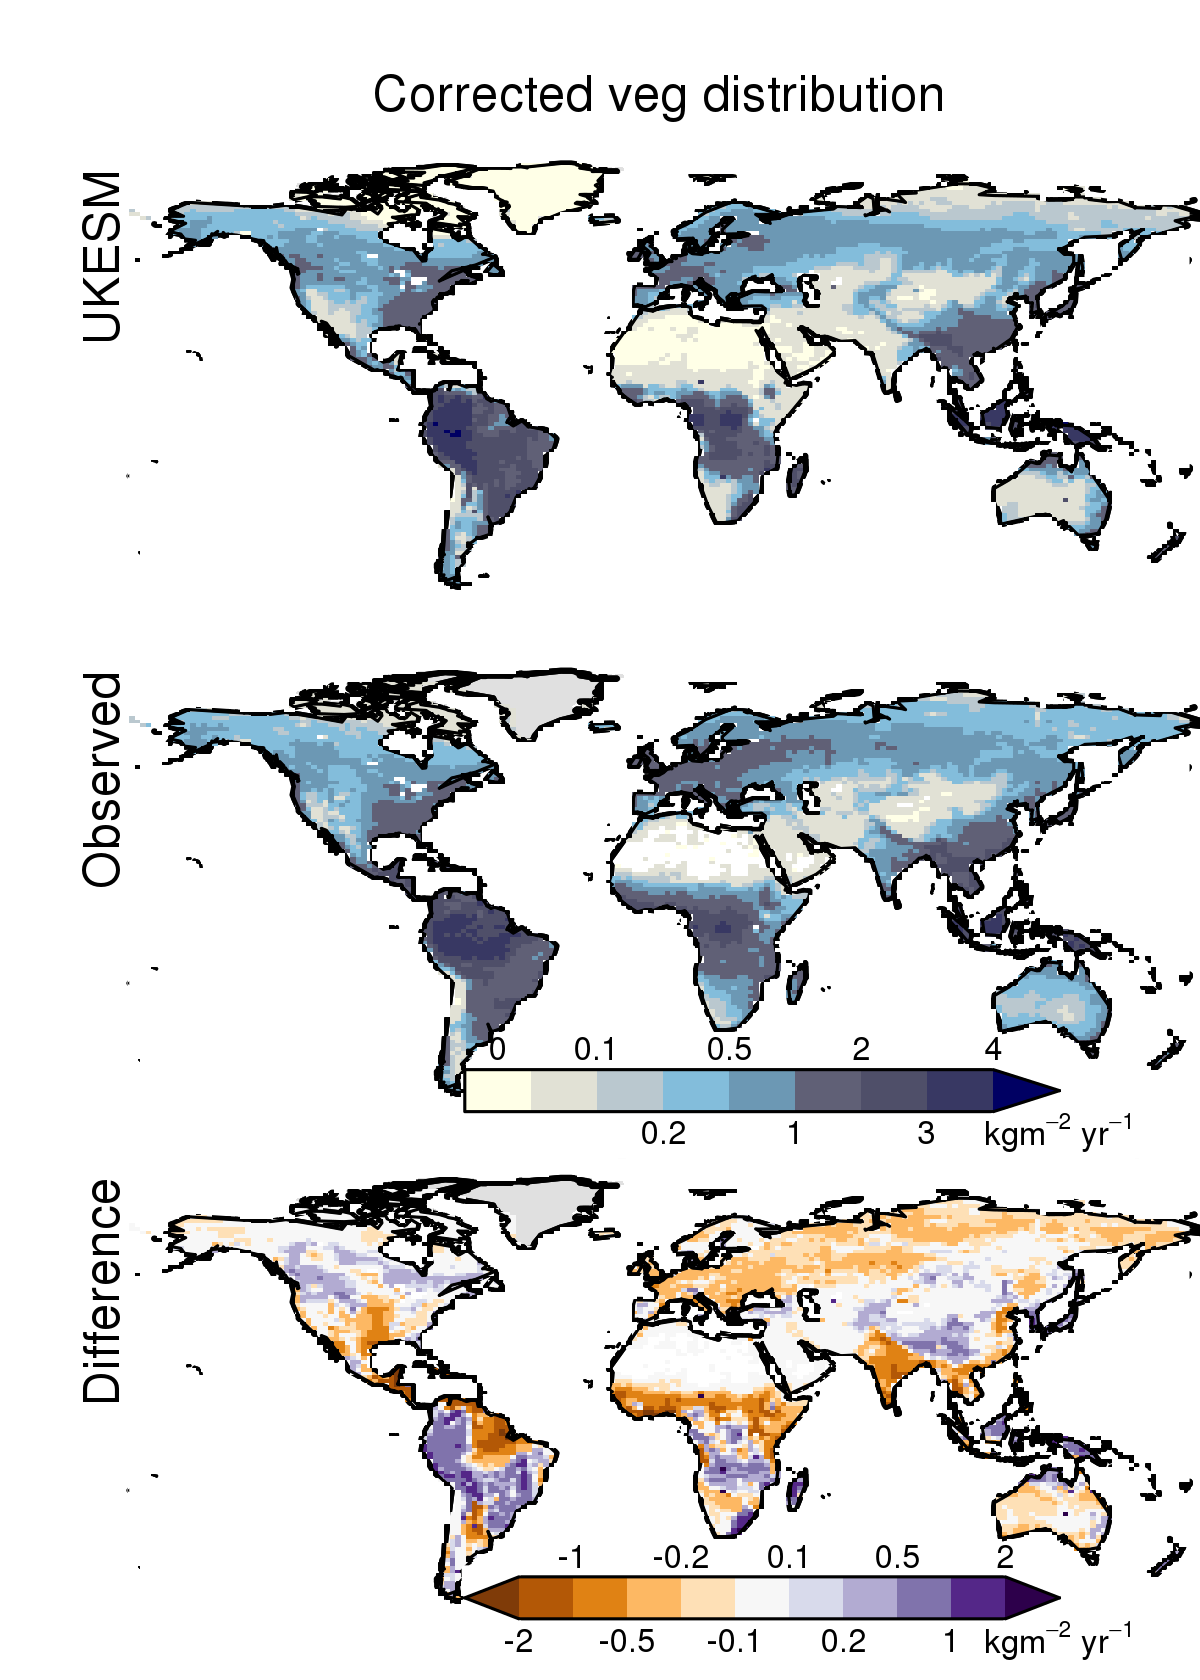
\includegraphics[width=5cm]{figs/GPP/fire_var_seasonality-maps-AA-mapsobsVegDist-gpp.png}
    
    %\end{subfigure}
    \caption{Simulated (top), observed (middle, <<ref>>) and different in mean annual GPP for 2001-2013. Right hand, UKESM has been corrected for vegetation distribution biases \label{fig:GPPmap}}
\end{figure*}

\begin{figure*}[t]
    %\begin{subfigure}
        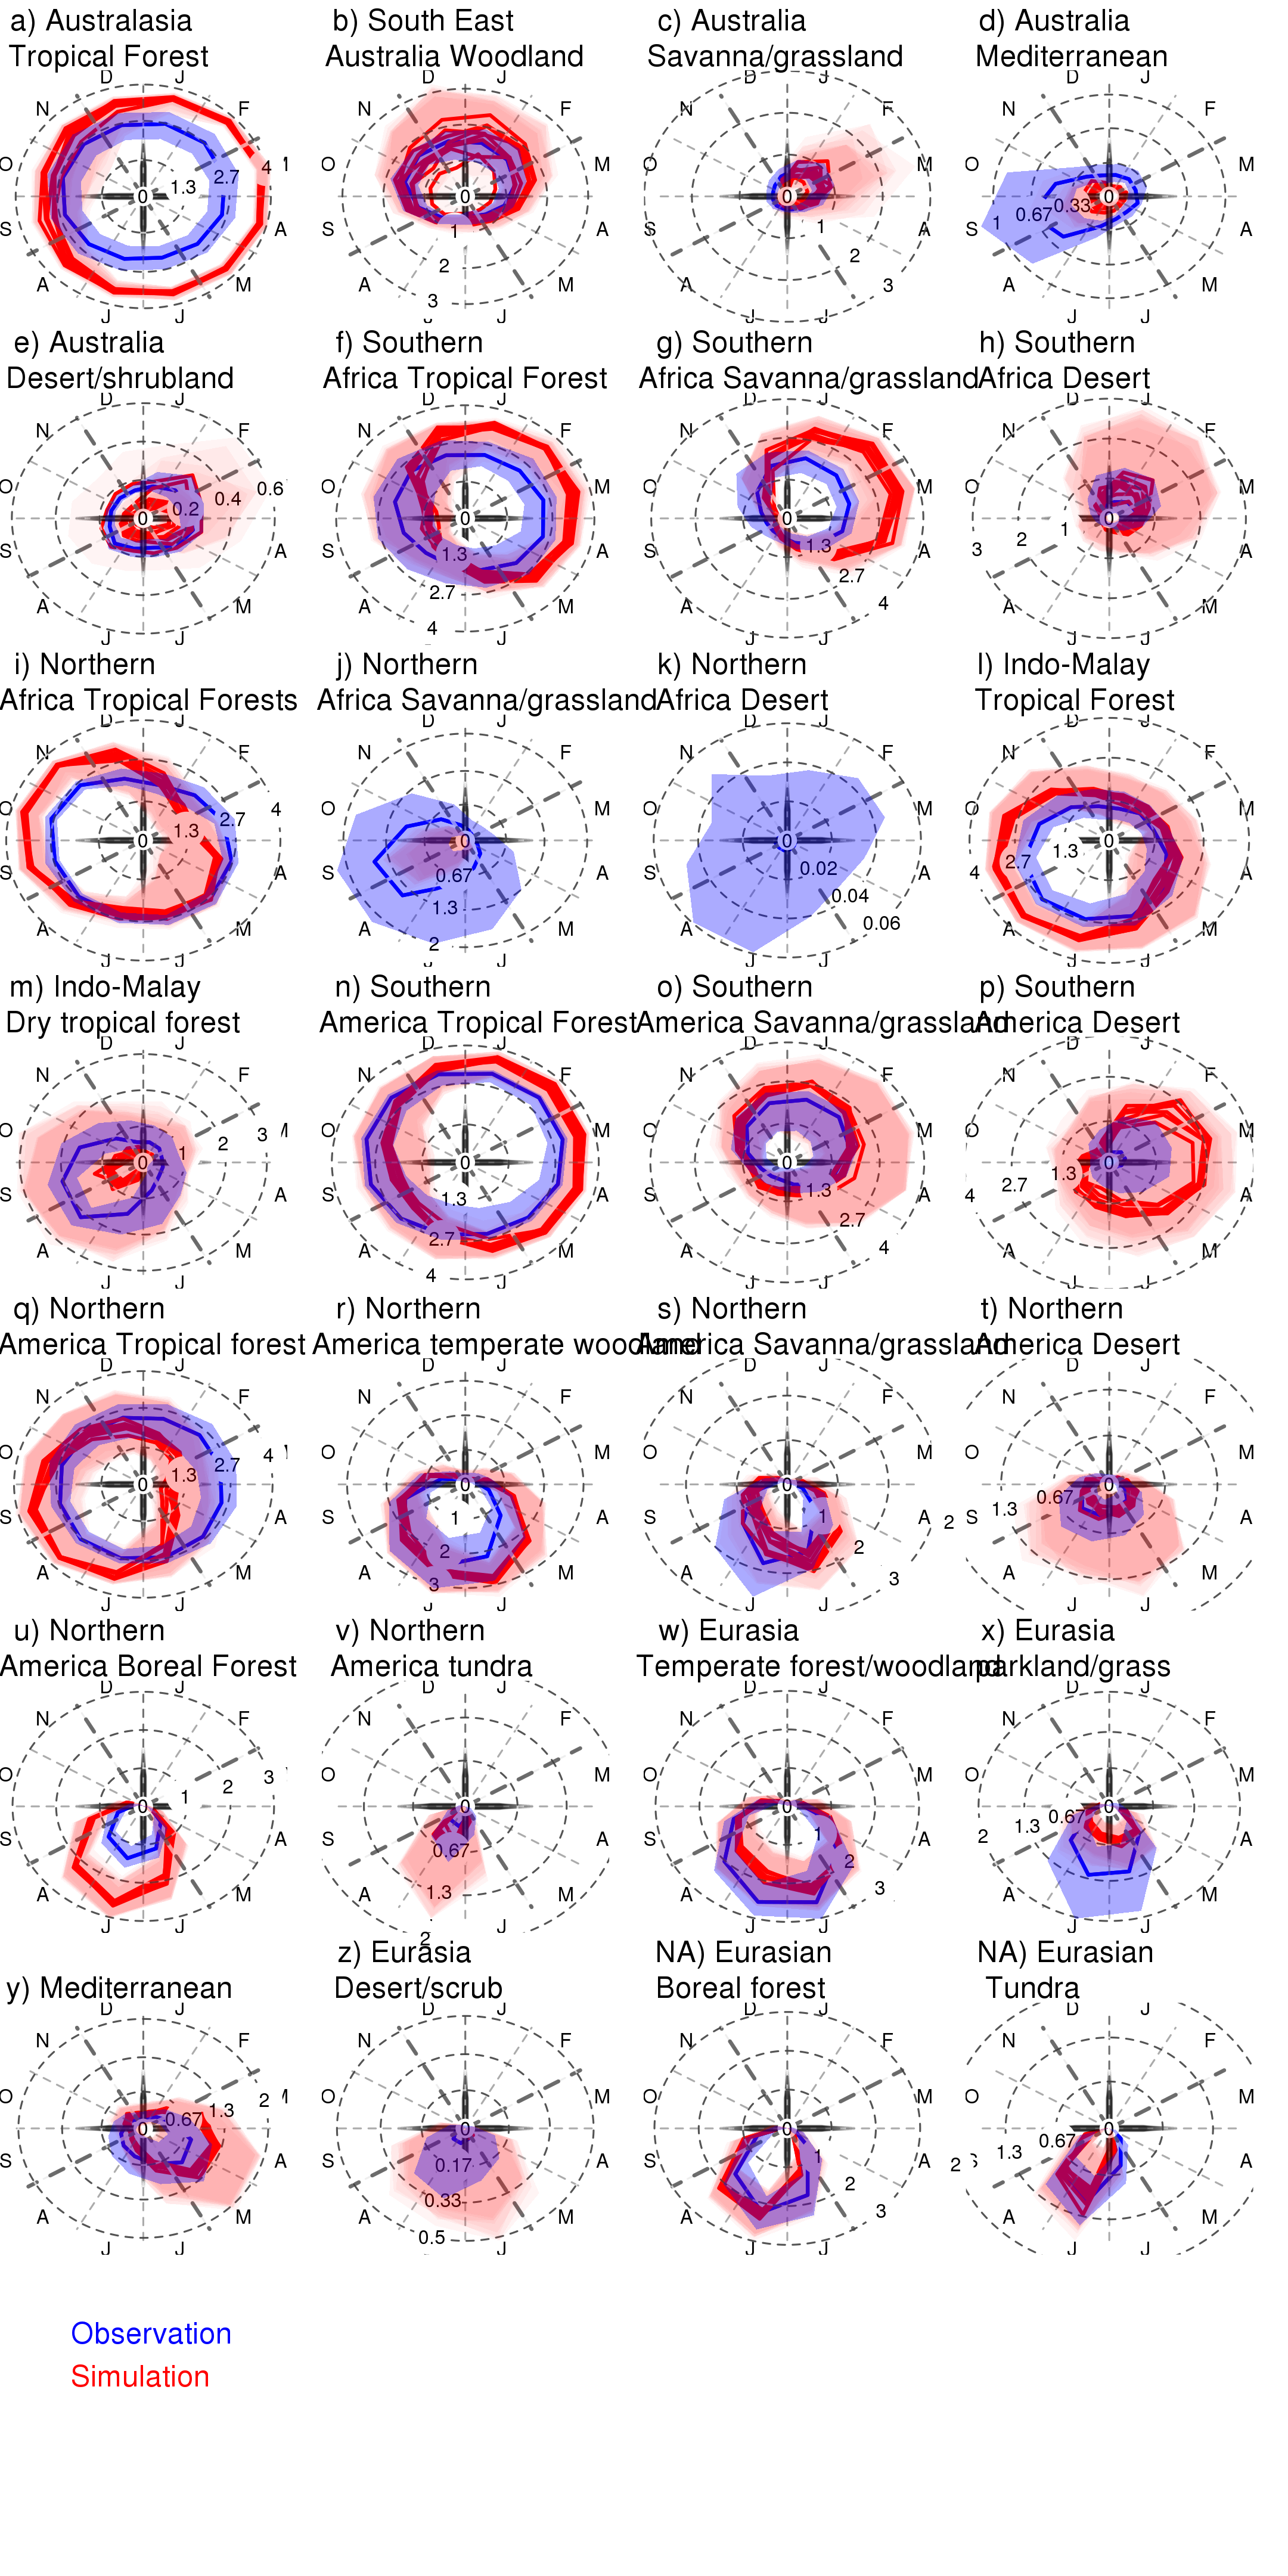
\includegraphics[width=5cm]{figs/GPP/fire_var_seasonality-TS-control-gpp.png}
    %\end{subfigure}
    %\begin{subfigure}
        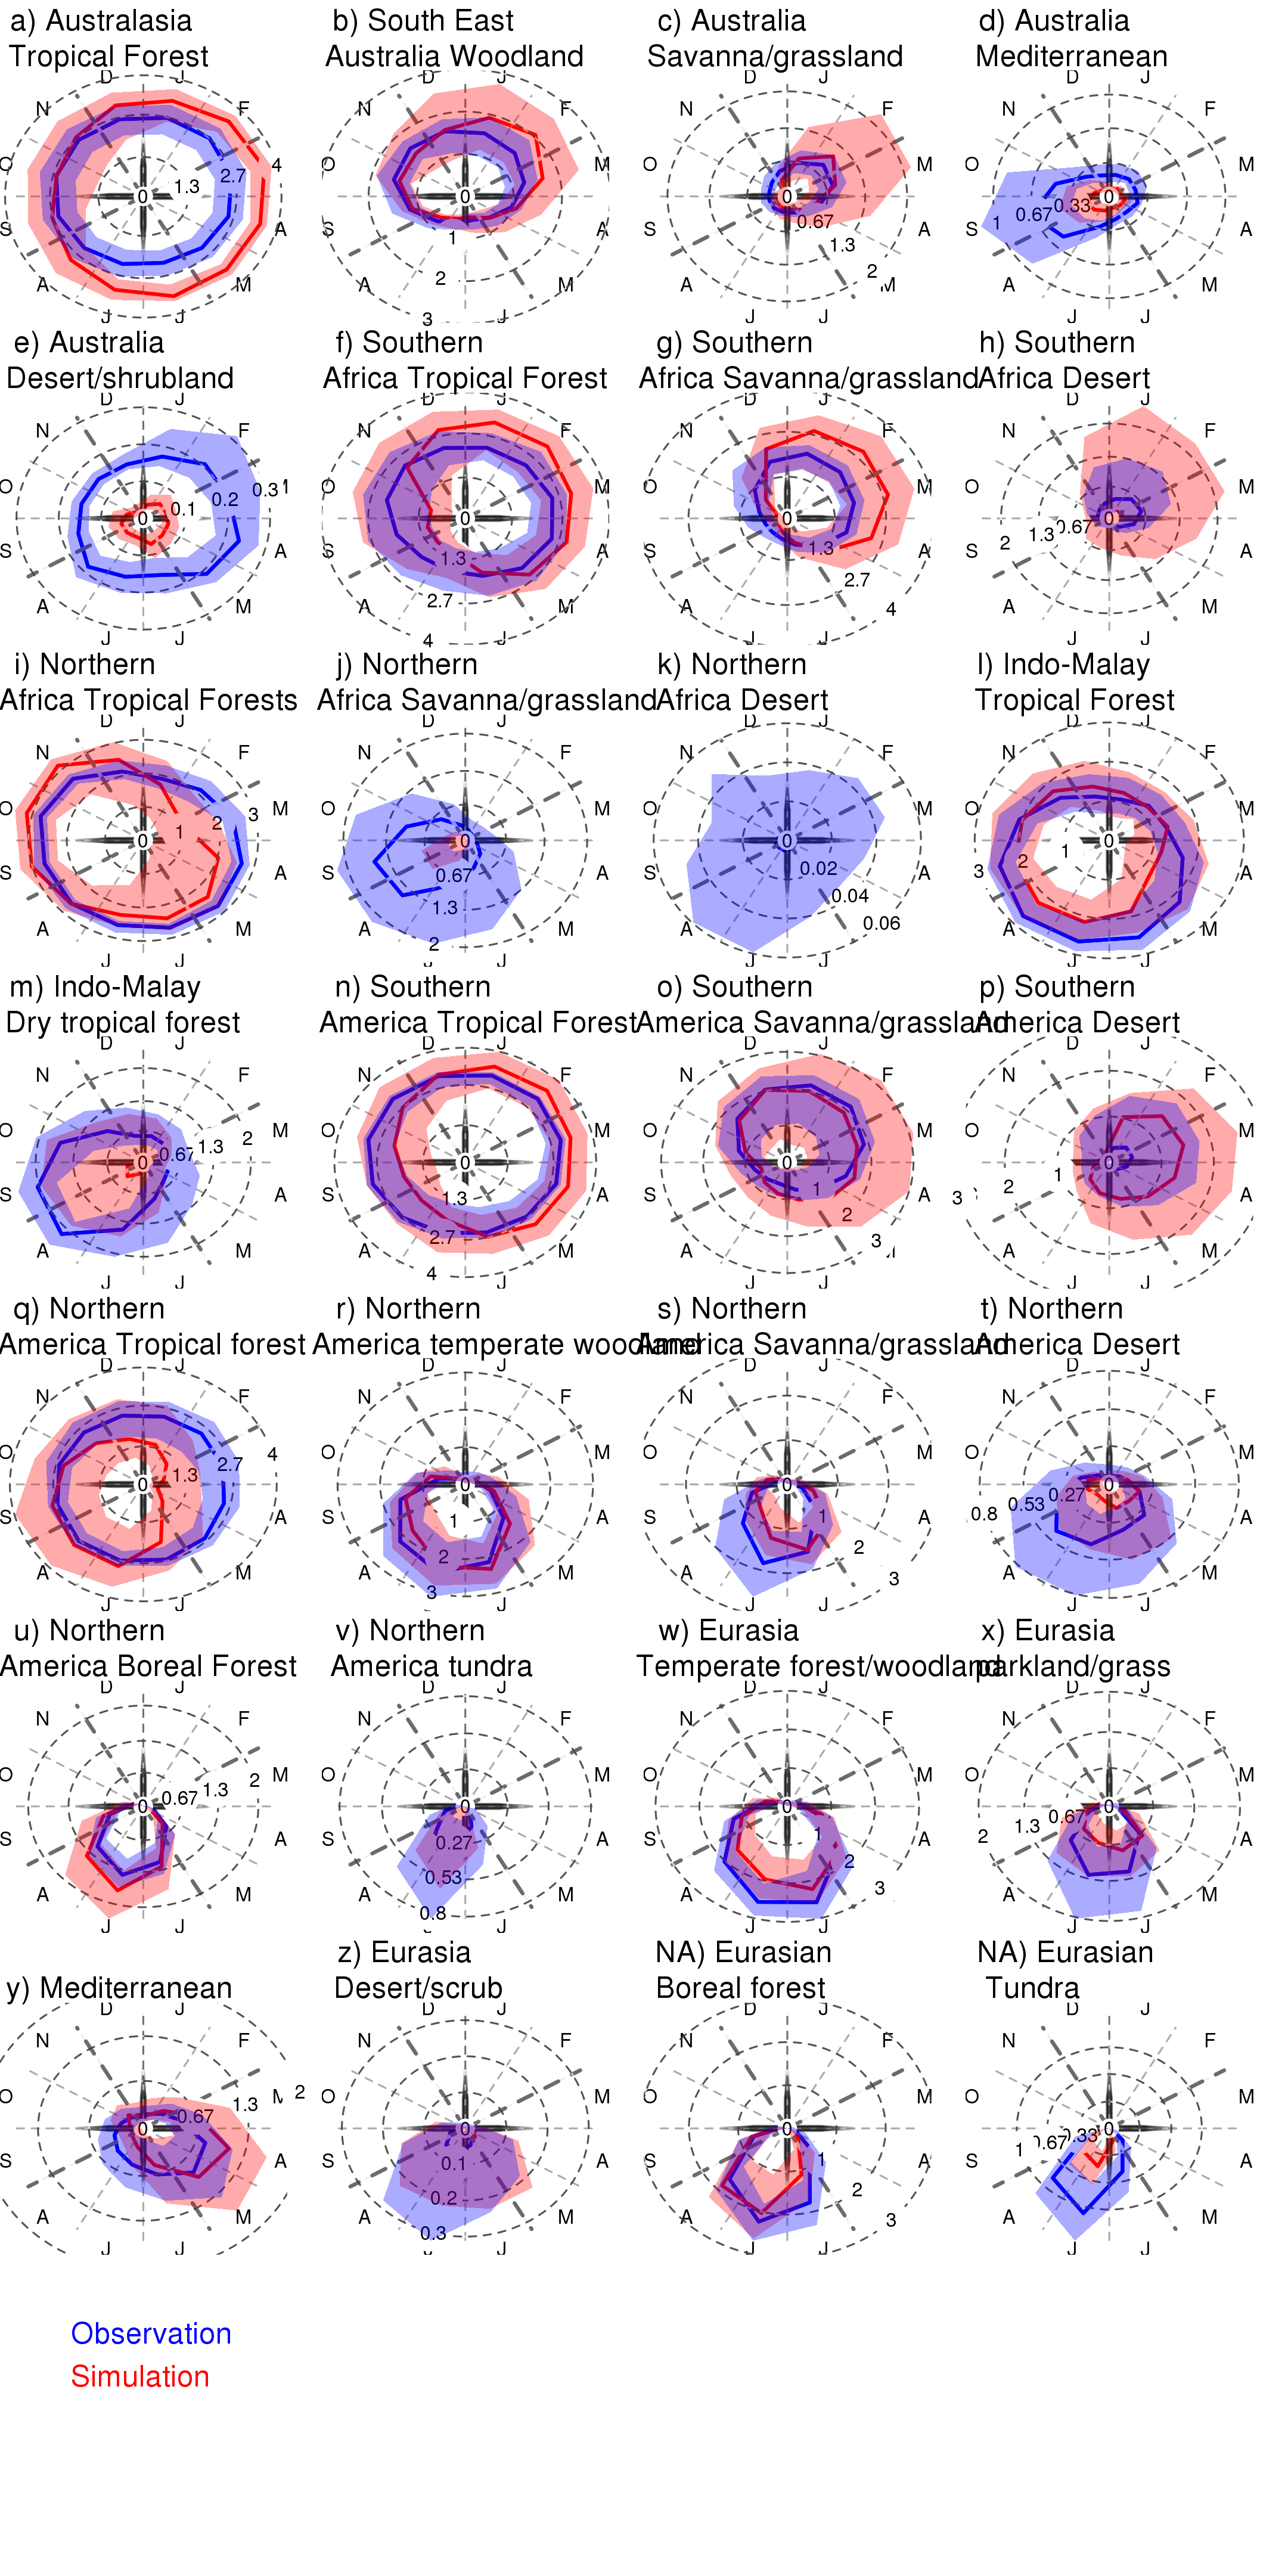
\includegraphics[width=5cm]{figs/GPP/fire_var_seasonality-TS-obsVegDist-gpp.png}
    
    %\end{subfigure}
    \caption{Simulated (red), observed (blue, <<ref>>) and seasonal cycles in GPP for 2001-2013 for each region(see \ref{fig:regionsMap}. Right hand, UKESM has been corrected for vegetation distribution biases \label{fig:GPPseasonalTS}}
\end{figure*}

\begin{figure*}[t]
    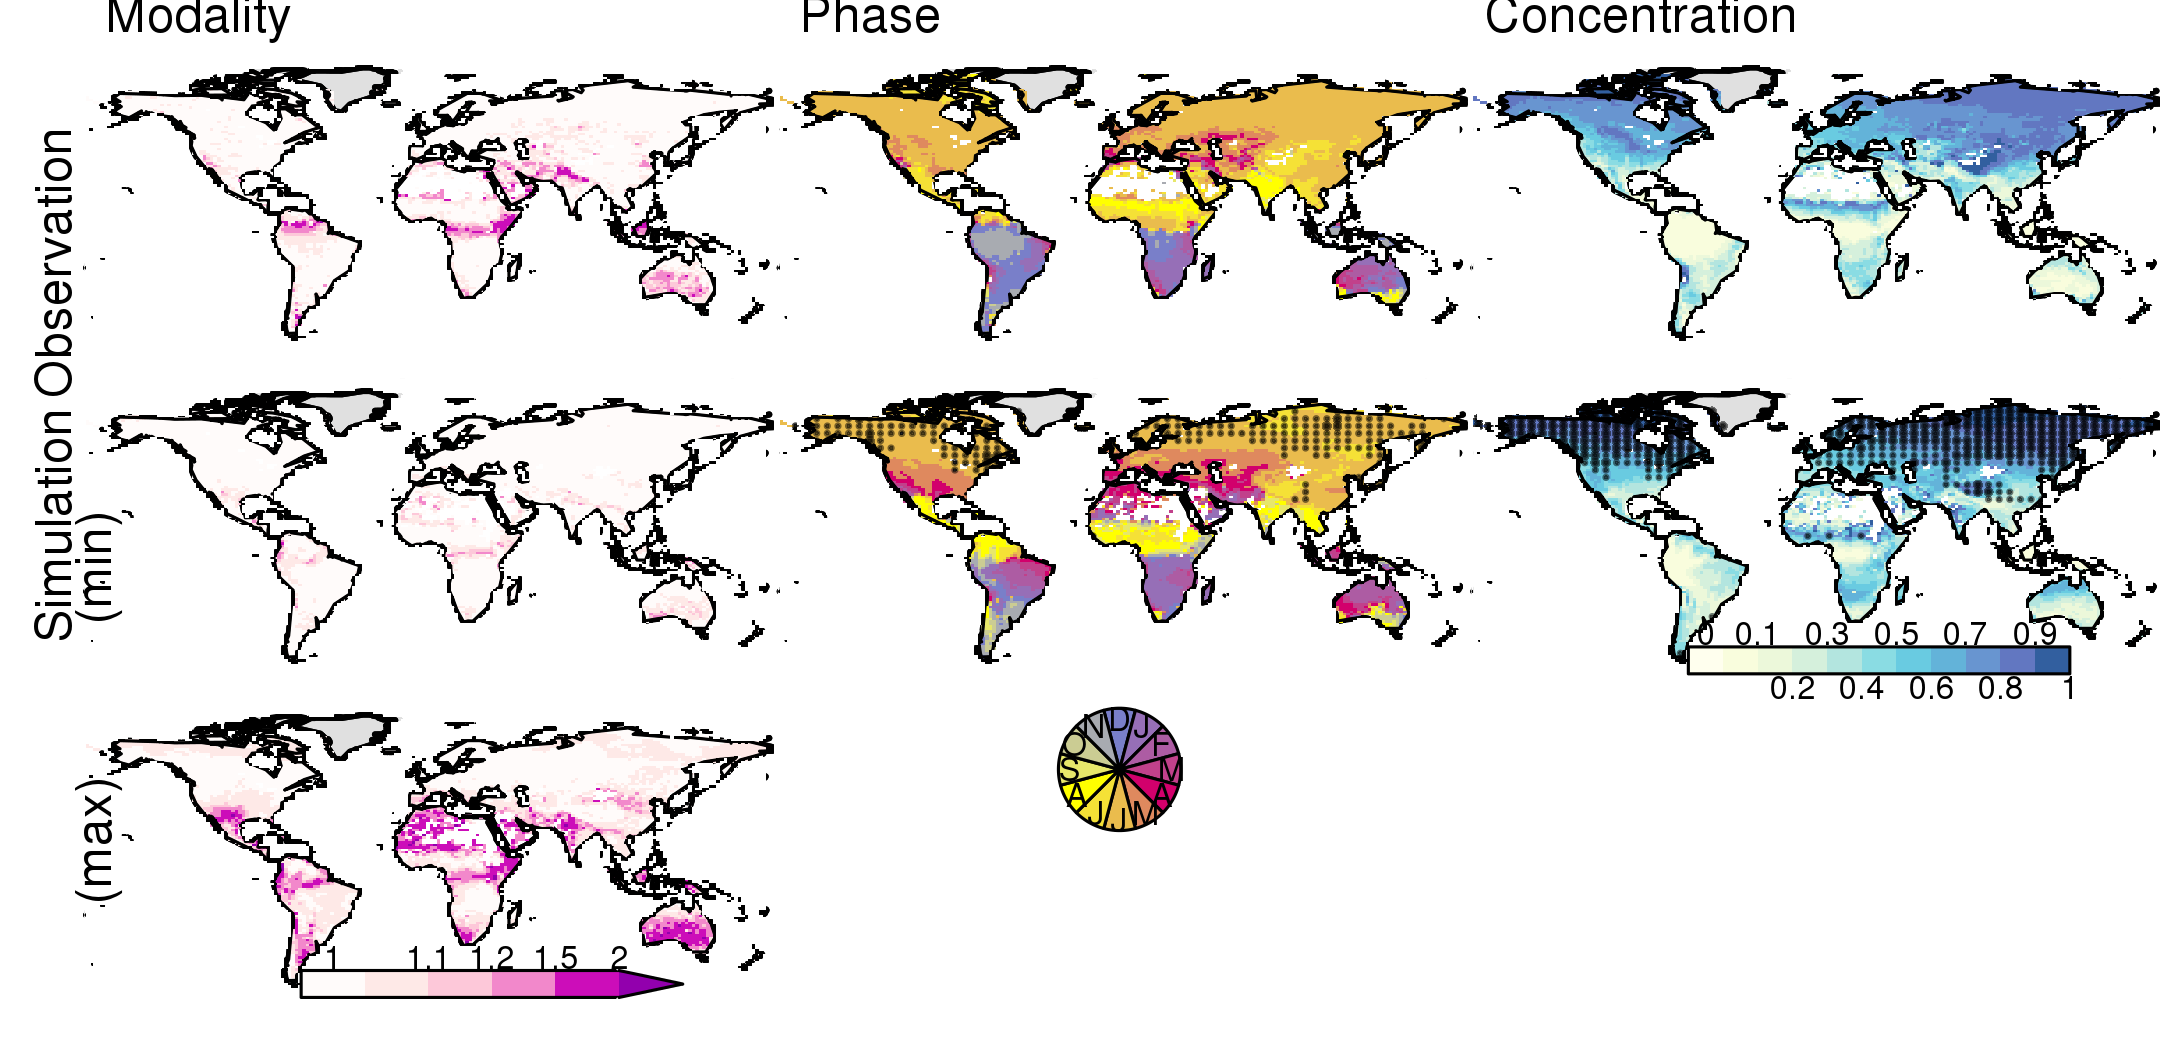
\includegraphics[width=12cm]{figs/GPP/fire_var_seasonality-maps-MPCcontrol-gpp.png}
    \caption{Seasonal comparison for GPP \label{fig:GPPseasonalMap}}
\end{figure*}


\subsubsection{Carbon turnover}
\hilight{Rebecca V - summary of results}

\begin{itemize}

	\item Globally the spatial pattern of both ecosystem carbon turnover and soil carbon turnover is reasonably well matched in UKESM1-0-LL compared with observations, which can be seen in the Figures `ecosystem tau map' and `soil tau map' respectively; however there is a bias towards longer turnover times in UKESM1-0-LL compared with the observational data. There are regions in the northern mid-latitudes which have noticeably long turnover times in UKESM1-0-LL, which is not seen in the observational figure. This seems to be due to corresponding large quantities of soil carbon seen in these regions, which again is not seen in the observational figure.This could be due to cSoil being related to vegetation or due to nitrogen decomposition? However, we note that globally the soil carbon turnover times in UKESM1-0-LL better match the observational data compared with the ecosystem carbon turnover times. In regions of the Northern latitudes, UKESM1-0-LL produces very long ecosystem turnover times which are greater than the corresponding soil carbon turnover times. This is likely to be a result of not an accurate representation of high latitude vegetation.
	
	\item We investigated the spatial sensitivity of both ecosystem carbon turnover ($\tau_\mathrm{e}$), and soil carbon turnover ($\tau_\mathrm{s}$) to temperature and precipitation, which can be seen in Figures `ecosystem tau scatterplot' and `soil tau scatterplot' respectively. These sensitivities were considered on a global scale and for the different biomes considered in this study (Tropical Evergreen Forest, Temperate Forest, Grassland, Mediterranean, Desert, Boreal Forest, Tundra). In all cases, spatial data (latitude / longitude) was plotted as follows: precipitation (y-axis) against temperature (x-axis), and then the data was coloured by the respective turnover, $\tau_\mathrm{e}$ and $\tau_\mathrm{s}$, values (colour bar). Globally the spatial pattern of the sensitivity of $\tau_\mathrm{e}$ and $\tau_\mathrm{s}$ to temperature and precipitation is reproduced in UKESM1-0-LL compared with observations. We investigate these sensitivities in individual biomes to locate where UKESM1-0-LL accurately matched observations, and where there are differences and model improvements are required.
	
	\item In the Tropical Evergreen Forest biome, UKESM1-0-LL matches well with the observations, with only a marginally slower turnover in observations. In Figure `ecosystem tau scatterplot' it can be seen that there are points with unusually long ecosystem carbon turnover times, which is likely to be due to the vegetation allocation in this biome.
	
	\item In the Grassland and Temperate Forest biomes, for both $\tau_\mathrm{e}$ and $\tau_\mathrm{s}$, UKESM1-0-LL generally has longer turnover times compared with observations. This could potentially be due to vegetation disturbances, UKESM1-0-LL is known to have harsh vegetation transitions, which might be causing no vegetation to be growing in some regions. Additionally, for both $\tau_\mathrm{e}$ and $\tau_\mathrm{s}$, there seems to be more of a temperature relationship to turnover seen in this biome in UKESM1-0-LL compared with the observations, whereas in observations there is more of a sensitivity to precipitation.
	
	\item In the Mediterranean biome, UKESM1-0-LL does not match the temperature and precipitation relationships to $\tau_\mathrm{e}$ and $\tau_\mathrm{s}$ as seen in observations. In the observations, lower precipitation and higher temperature results in a longer carbon turnover, whereas the opposite affect is seen in UKESM1-0-LL.
	
	\item The Desert and Boreal Forest biomes are exceptions where UKESM1-0-LL does not produce slower carbon turnover compared with observations. In the Desert biome, a stronger temperature sensitivity on carbon turnover is seen in UKESM1-0-LL compared with observations, whereas a stronger precipitation sensitivity is seen in observations. This precipitation sensitivity is partly seen for $\tau_\mathrm{s}$, however is not seen at all for $\tau_\mathrm{e}$, which means it is likely to be due to wrong vegetation here? In the Boreal Forest biome, long carbon turnover times are seen in the observations, with a sensitivity to temperature within the biome, both of these are not seen in UKESM1-0-LL. Within UKESM1-0-LL, there is a slight precipitation sensitivity seen in this biome, though less variation in turnover is seen compared to observations.

	\item In the Tundra biome however, a greater variation of turnover is seen within the biome in UKESM1-0-LL compared with observations, due to a more apparent temperature sensitivity of turnover in UKESM1-0-LL. Again, this could be due to not an accurate representation of high latitude vegetation.
	
	\item \textit{We note our results are dependent on the choice of benchmark observational datasets (cite tau uncertainty paper).}

\end{itemize}



\begin{figure*}[t]
    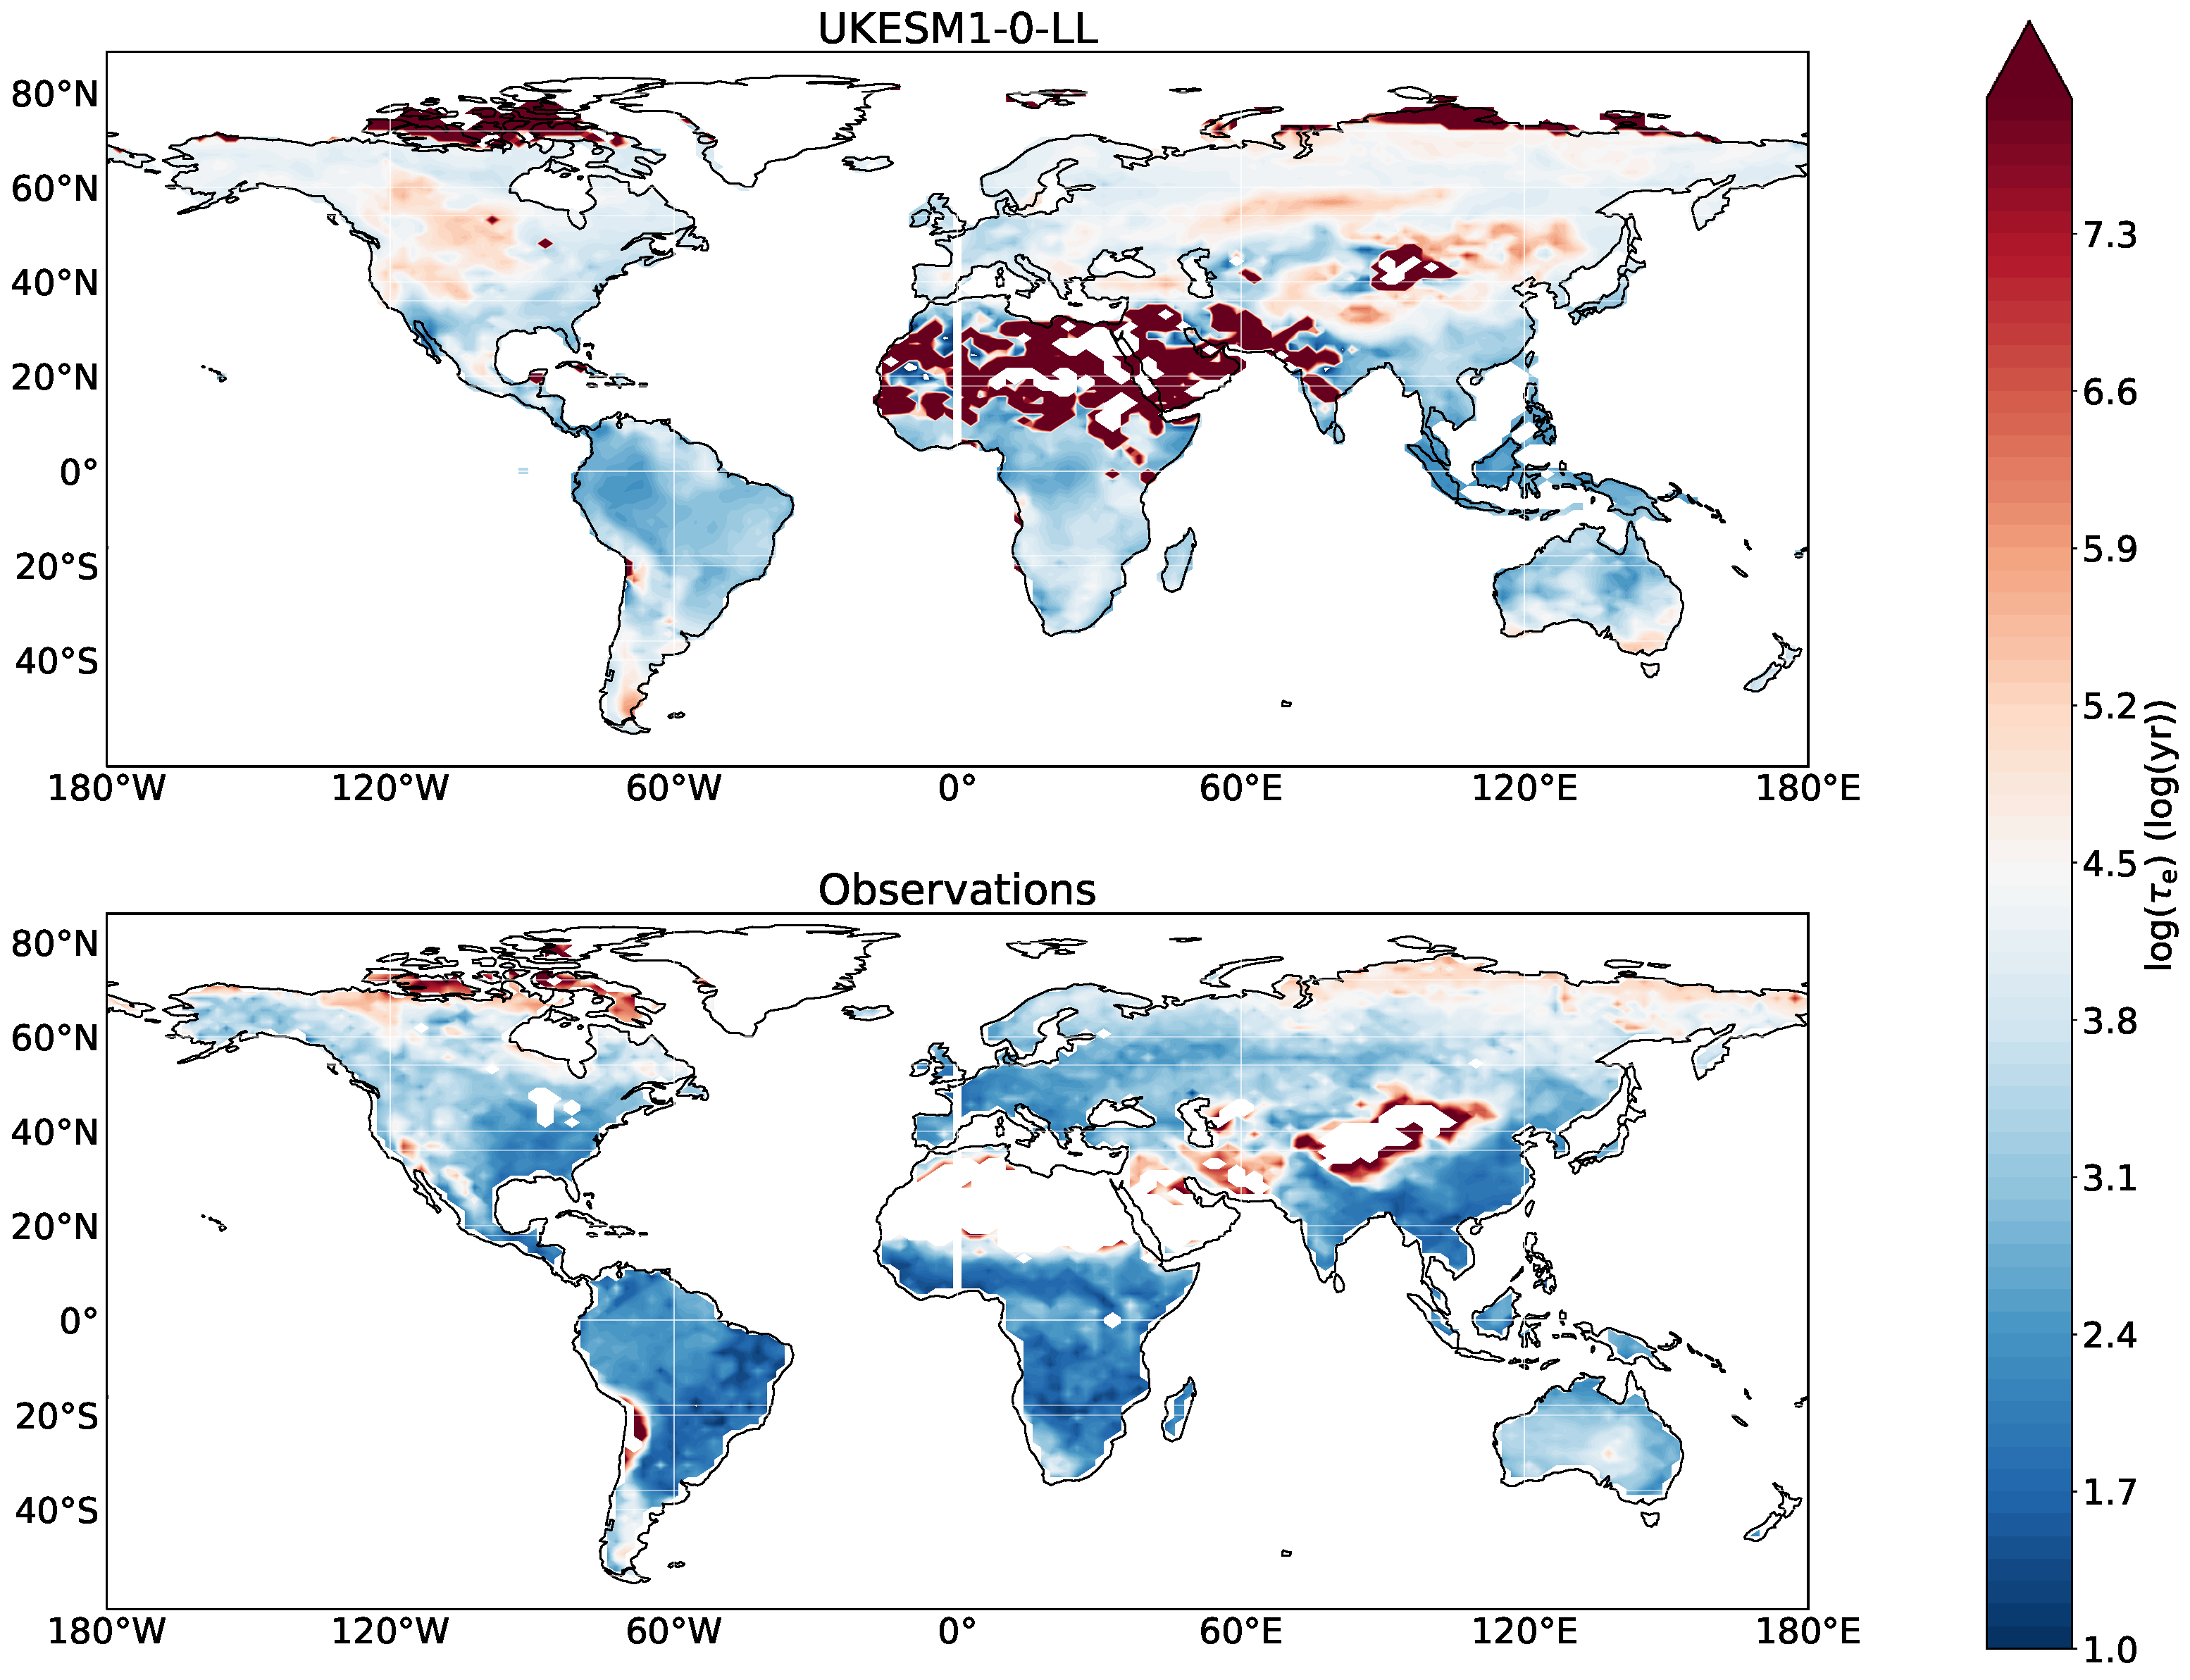
\includegraphics[width=12cm]{figs/Turnover/ecosystem_tau_map_comparison.pdf}
    \caption{Ecosystem turnover \label{fig:EcoTurnoverlMap}}
\end{figure*}

\begin{figure*}[t]
    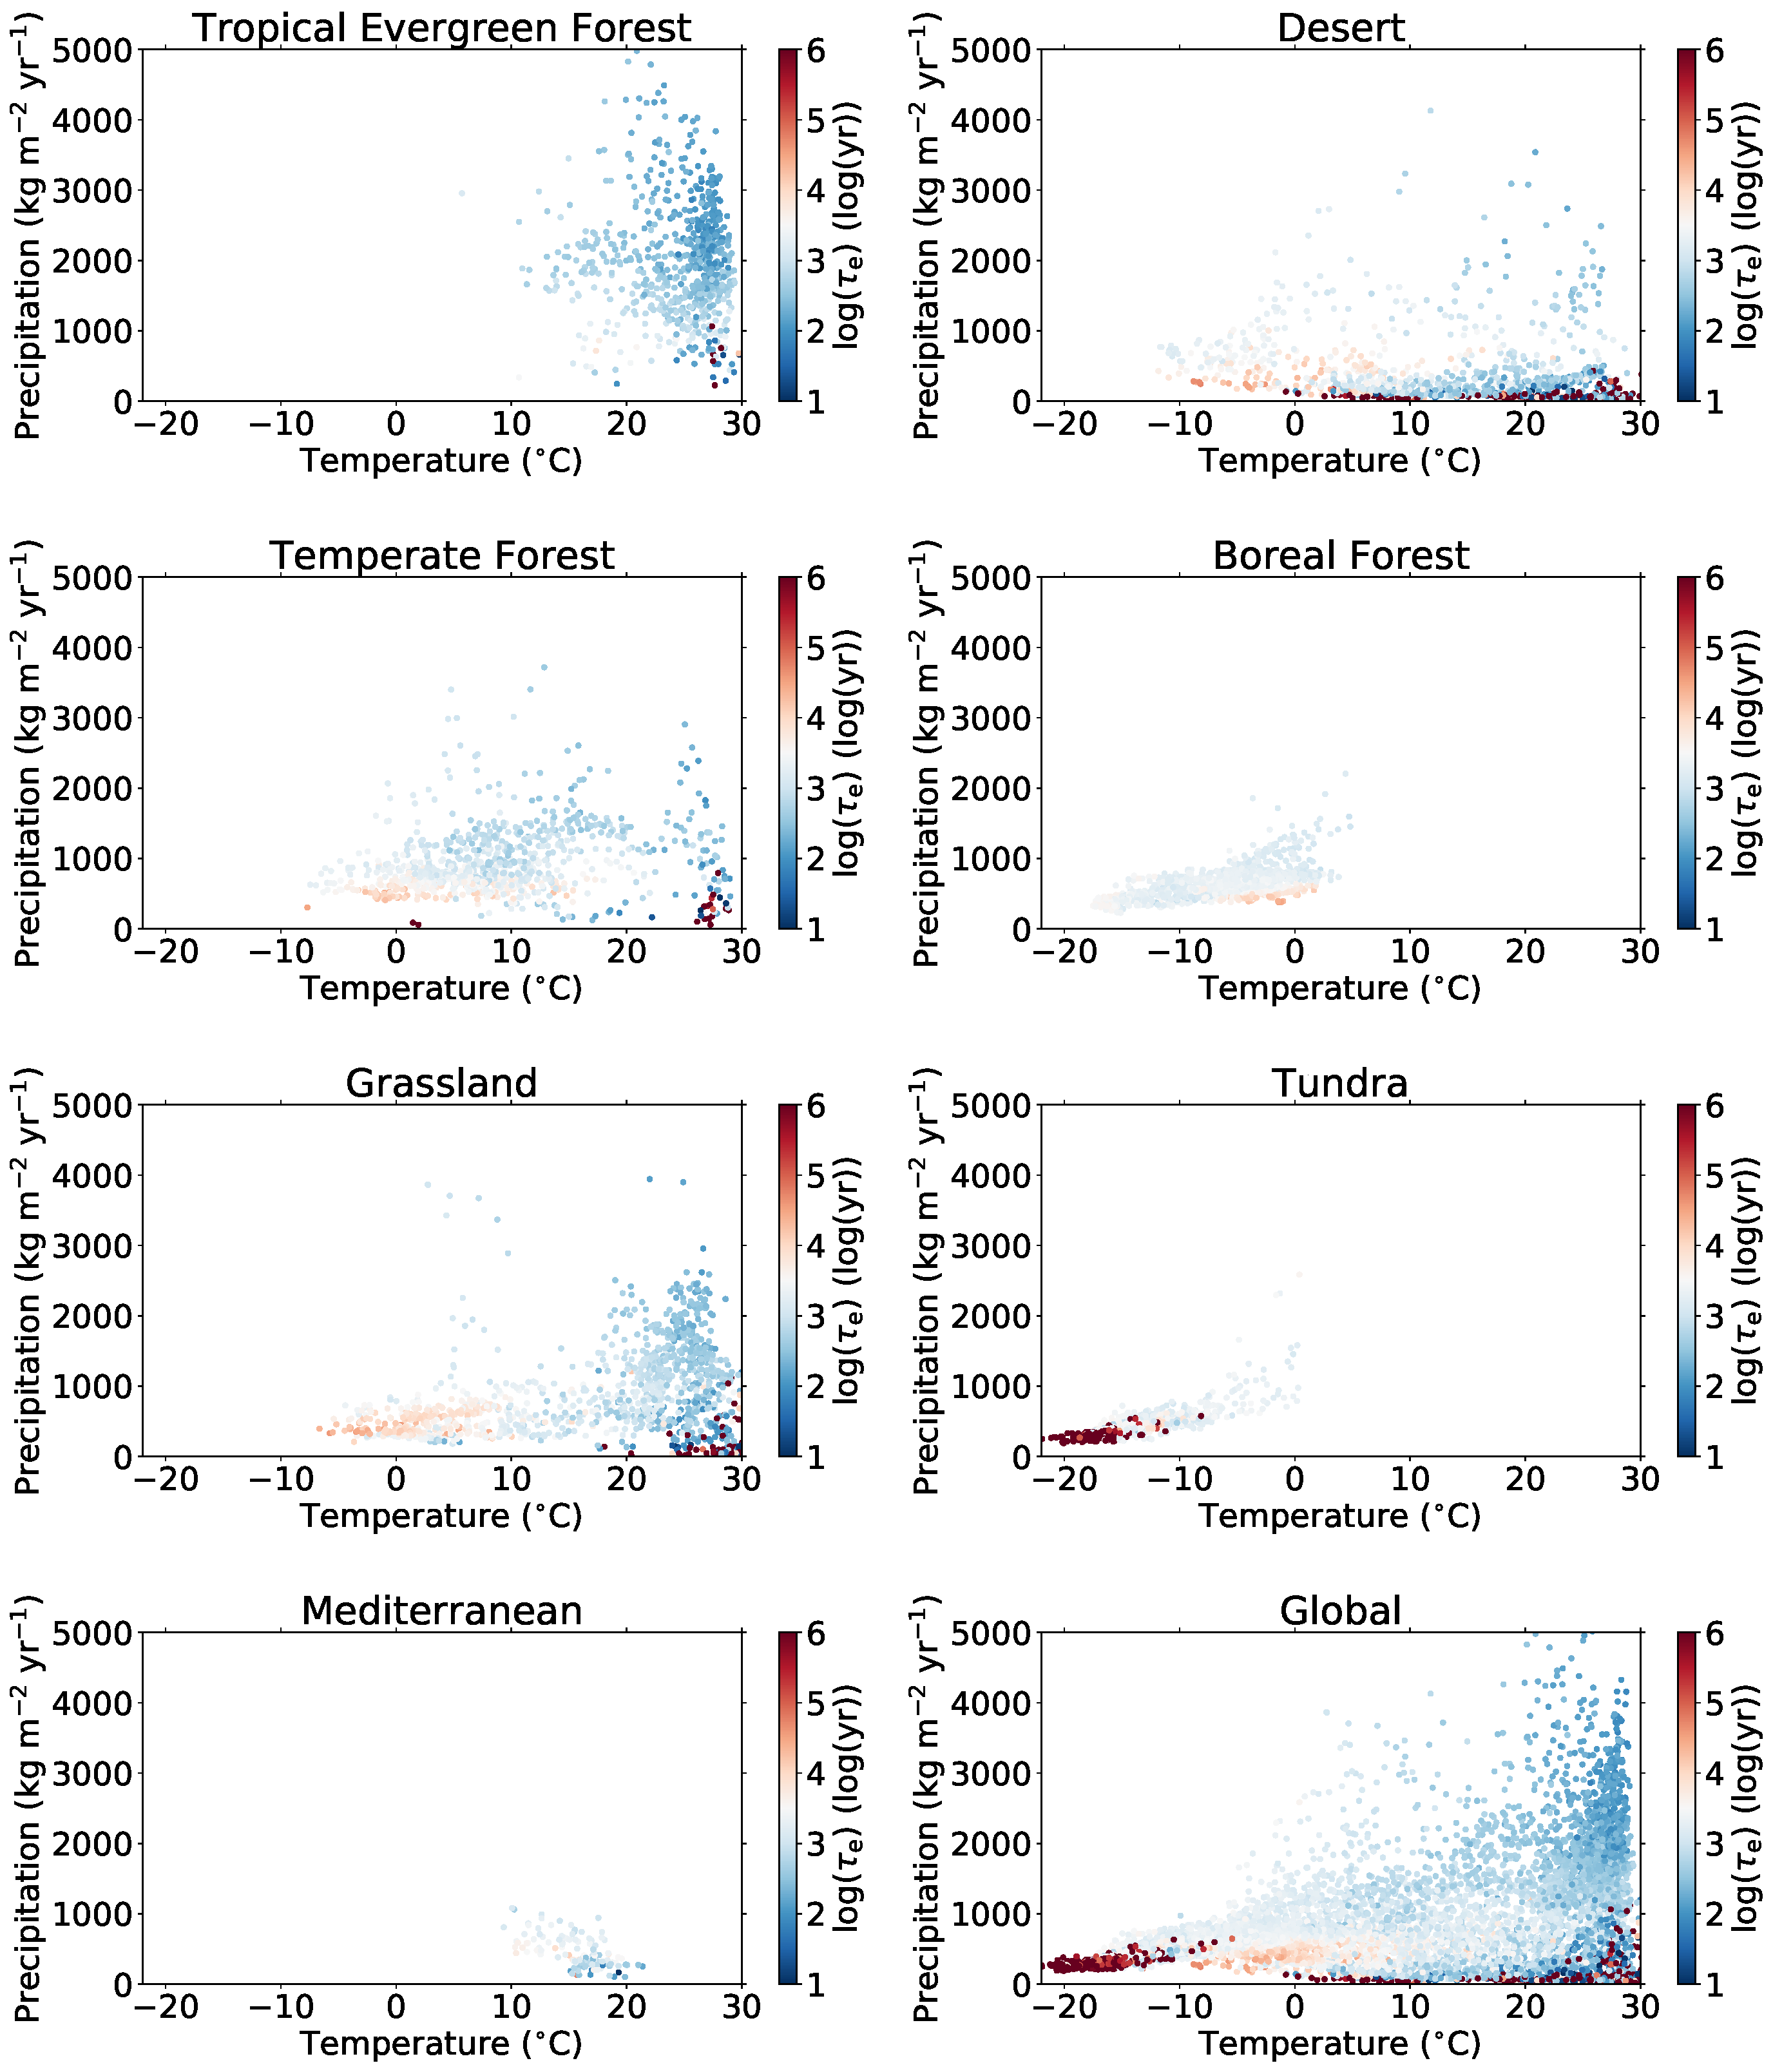
\includegraphics[width=6cm]{figs/Turnover/UKESM_ecosystem_colouredbytau_biome_log.pdf}
    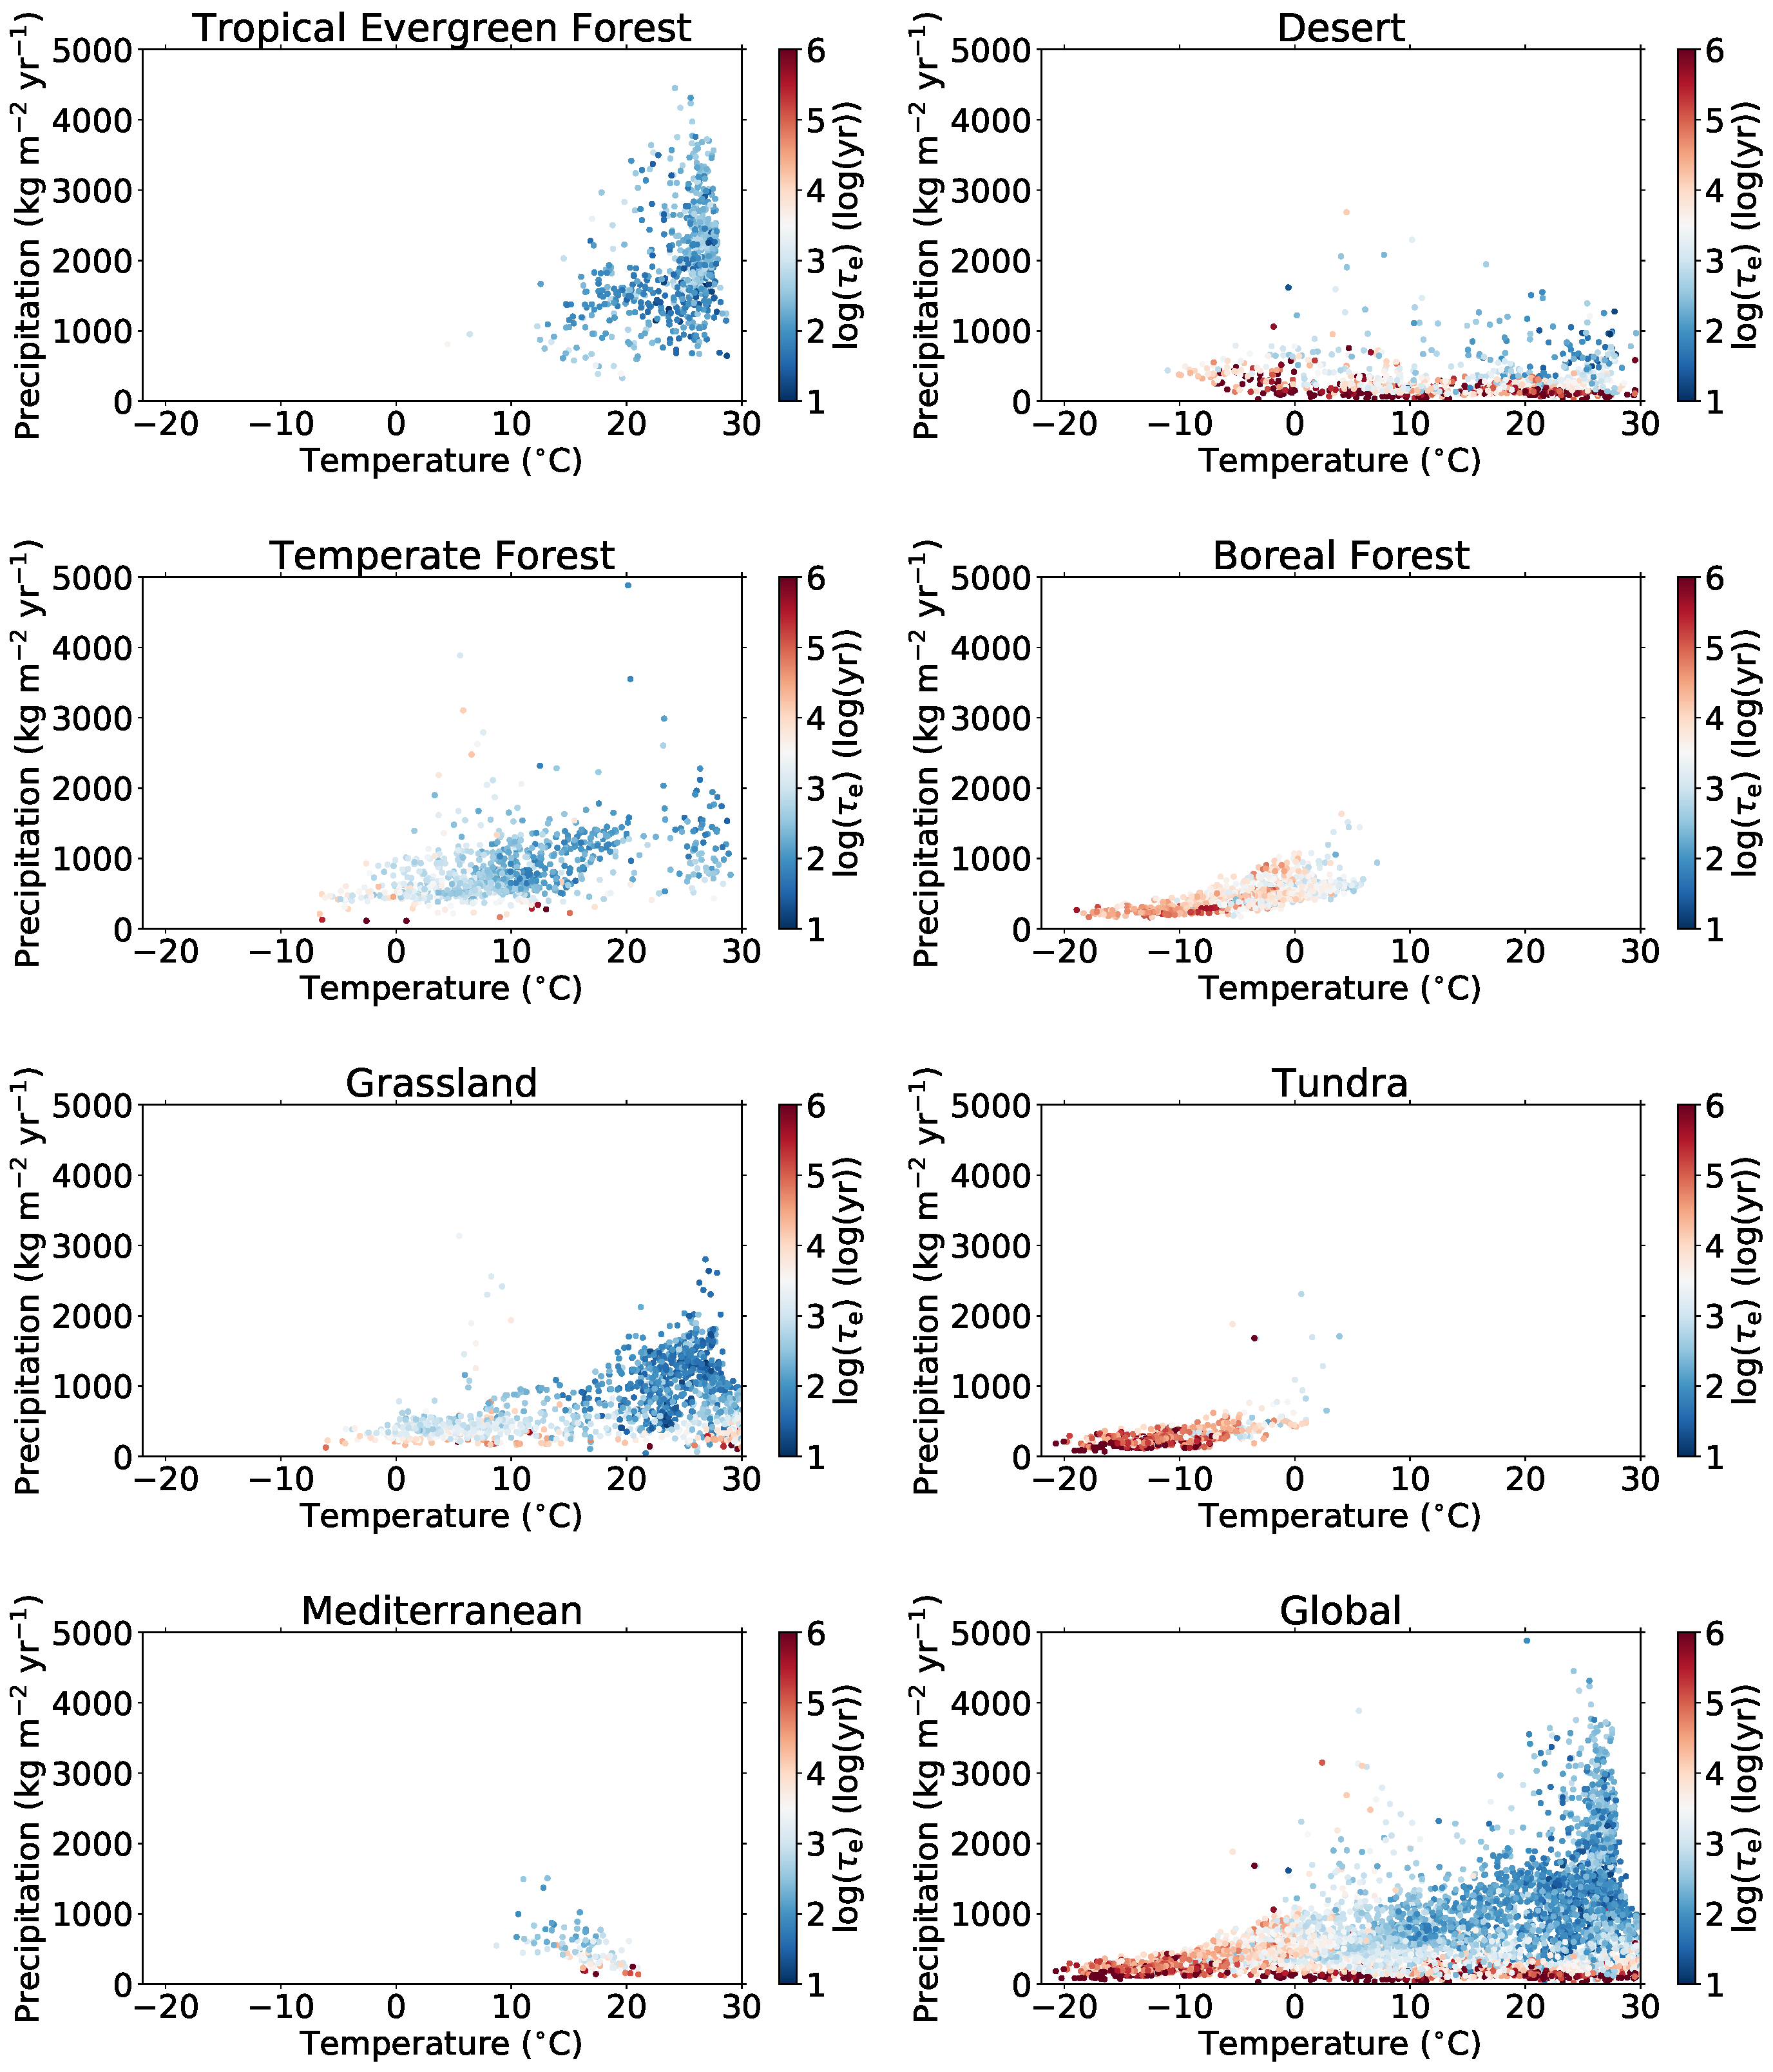
\includegraphics[width=6cm]{figs/Turnover/obs1_ecosystem_colouredbytau_biome_log.pdf}
    \caption{Ecosystem turnover \label{fig:EcoTurnoverScatter}}
\end{figure*}

\begin{figure*}[t]
    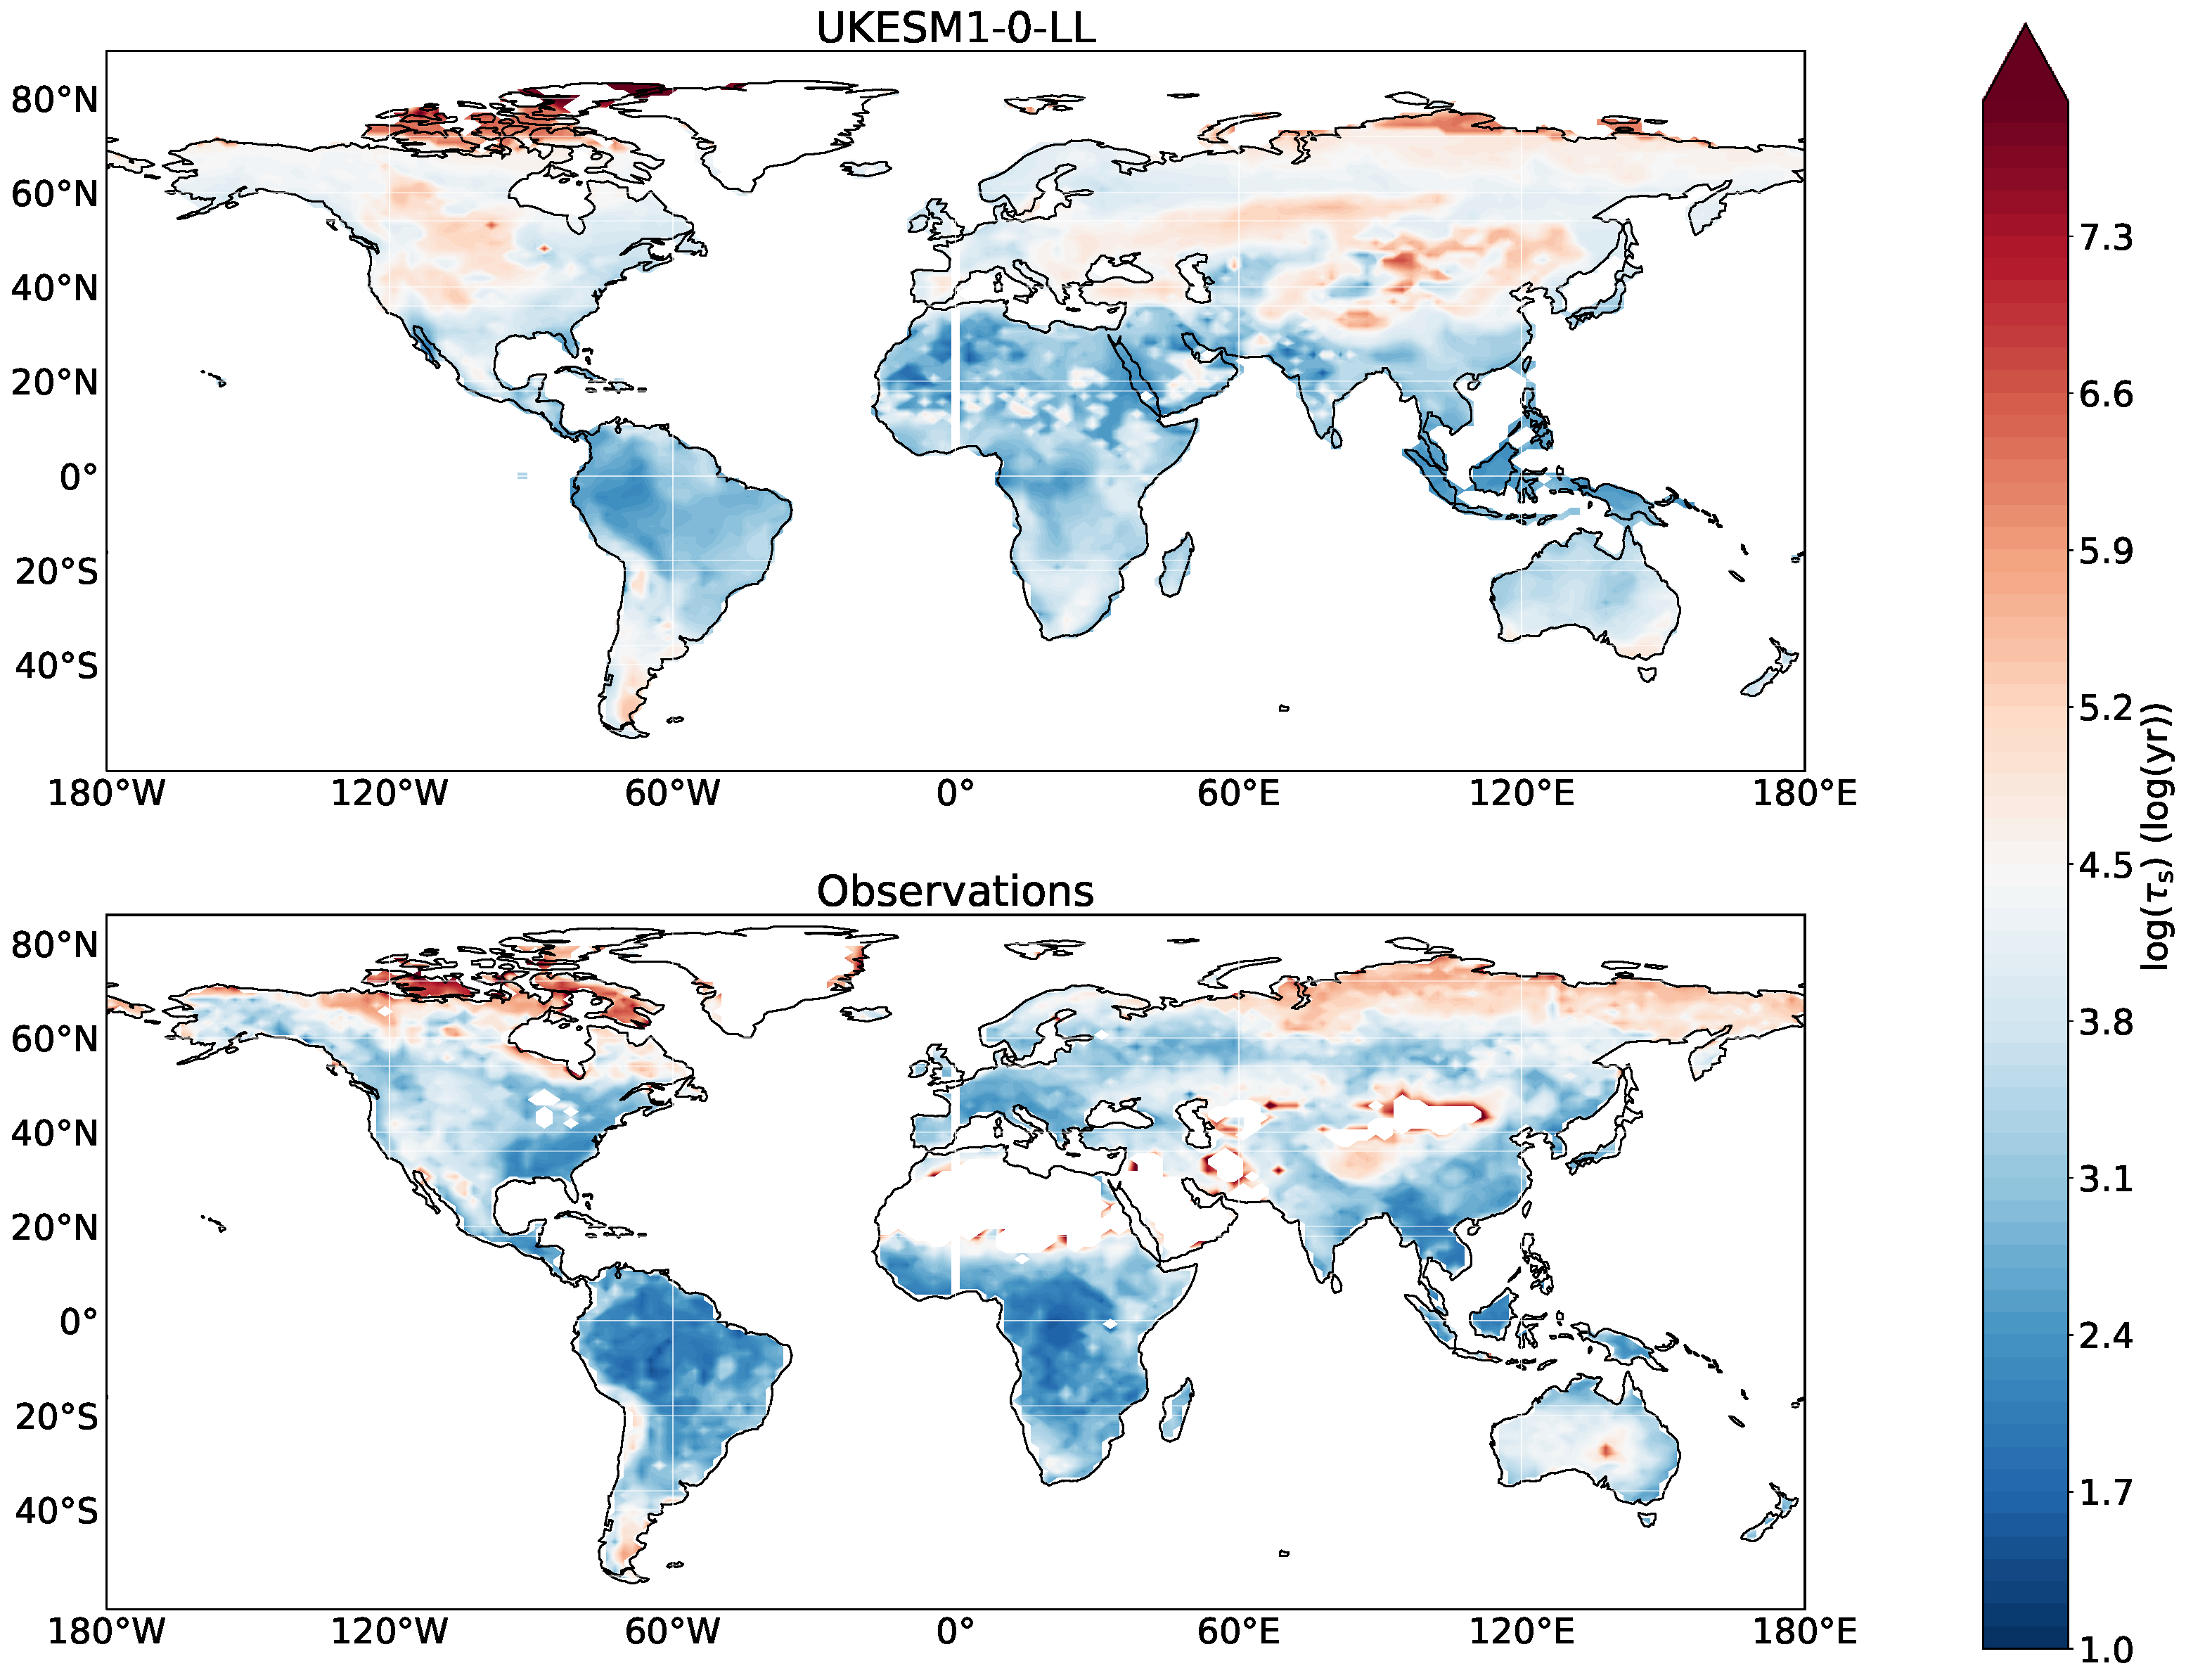
\includegraphics[width=12cm]{figs/Turnover/soil_tau_map_comparison.pdf}
    \caption{Soil turnover \label{fig:SoilTurnoverlMap}}
\end{figure*}

\begin{figure*}[t]
    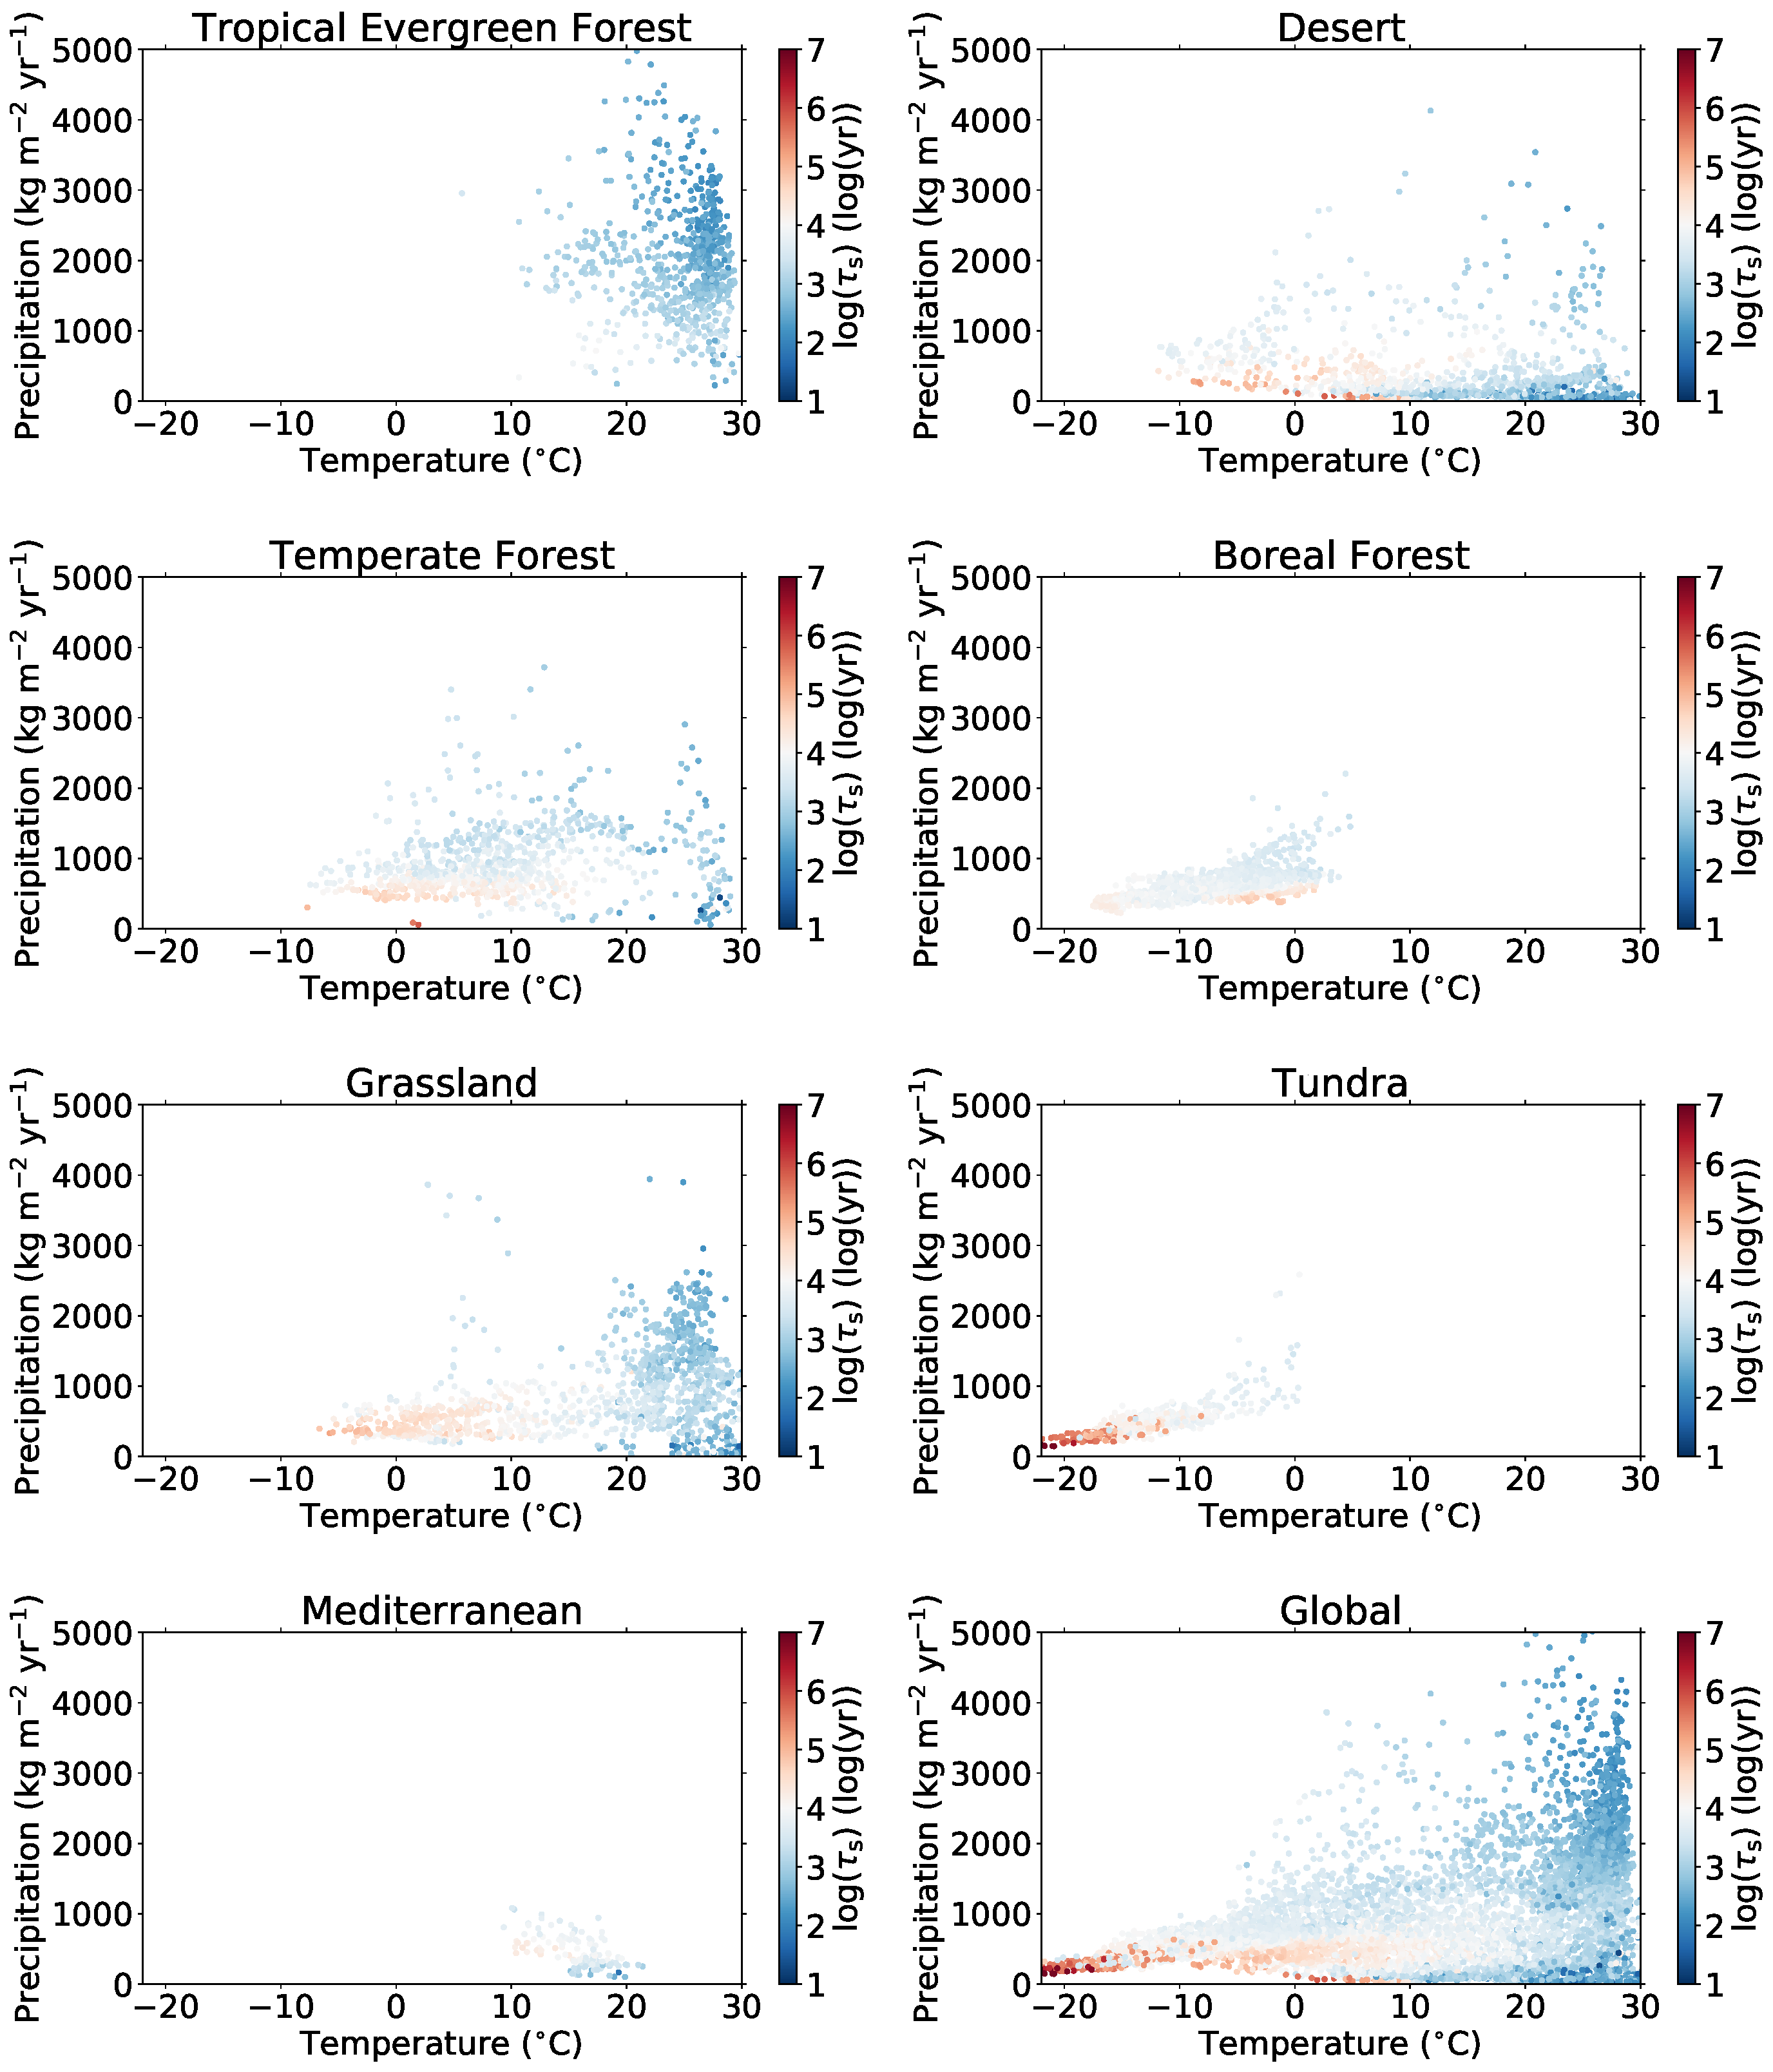
\includegraphics[width=6cm]{figs/Turnover/soil_UKESM_colouredbytau_biome_log.pdf}
    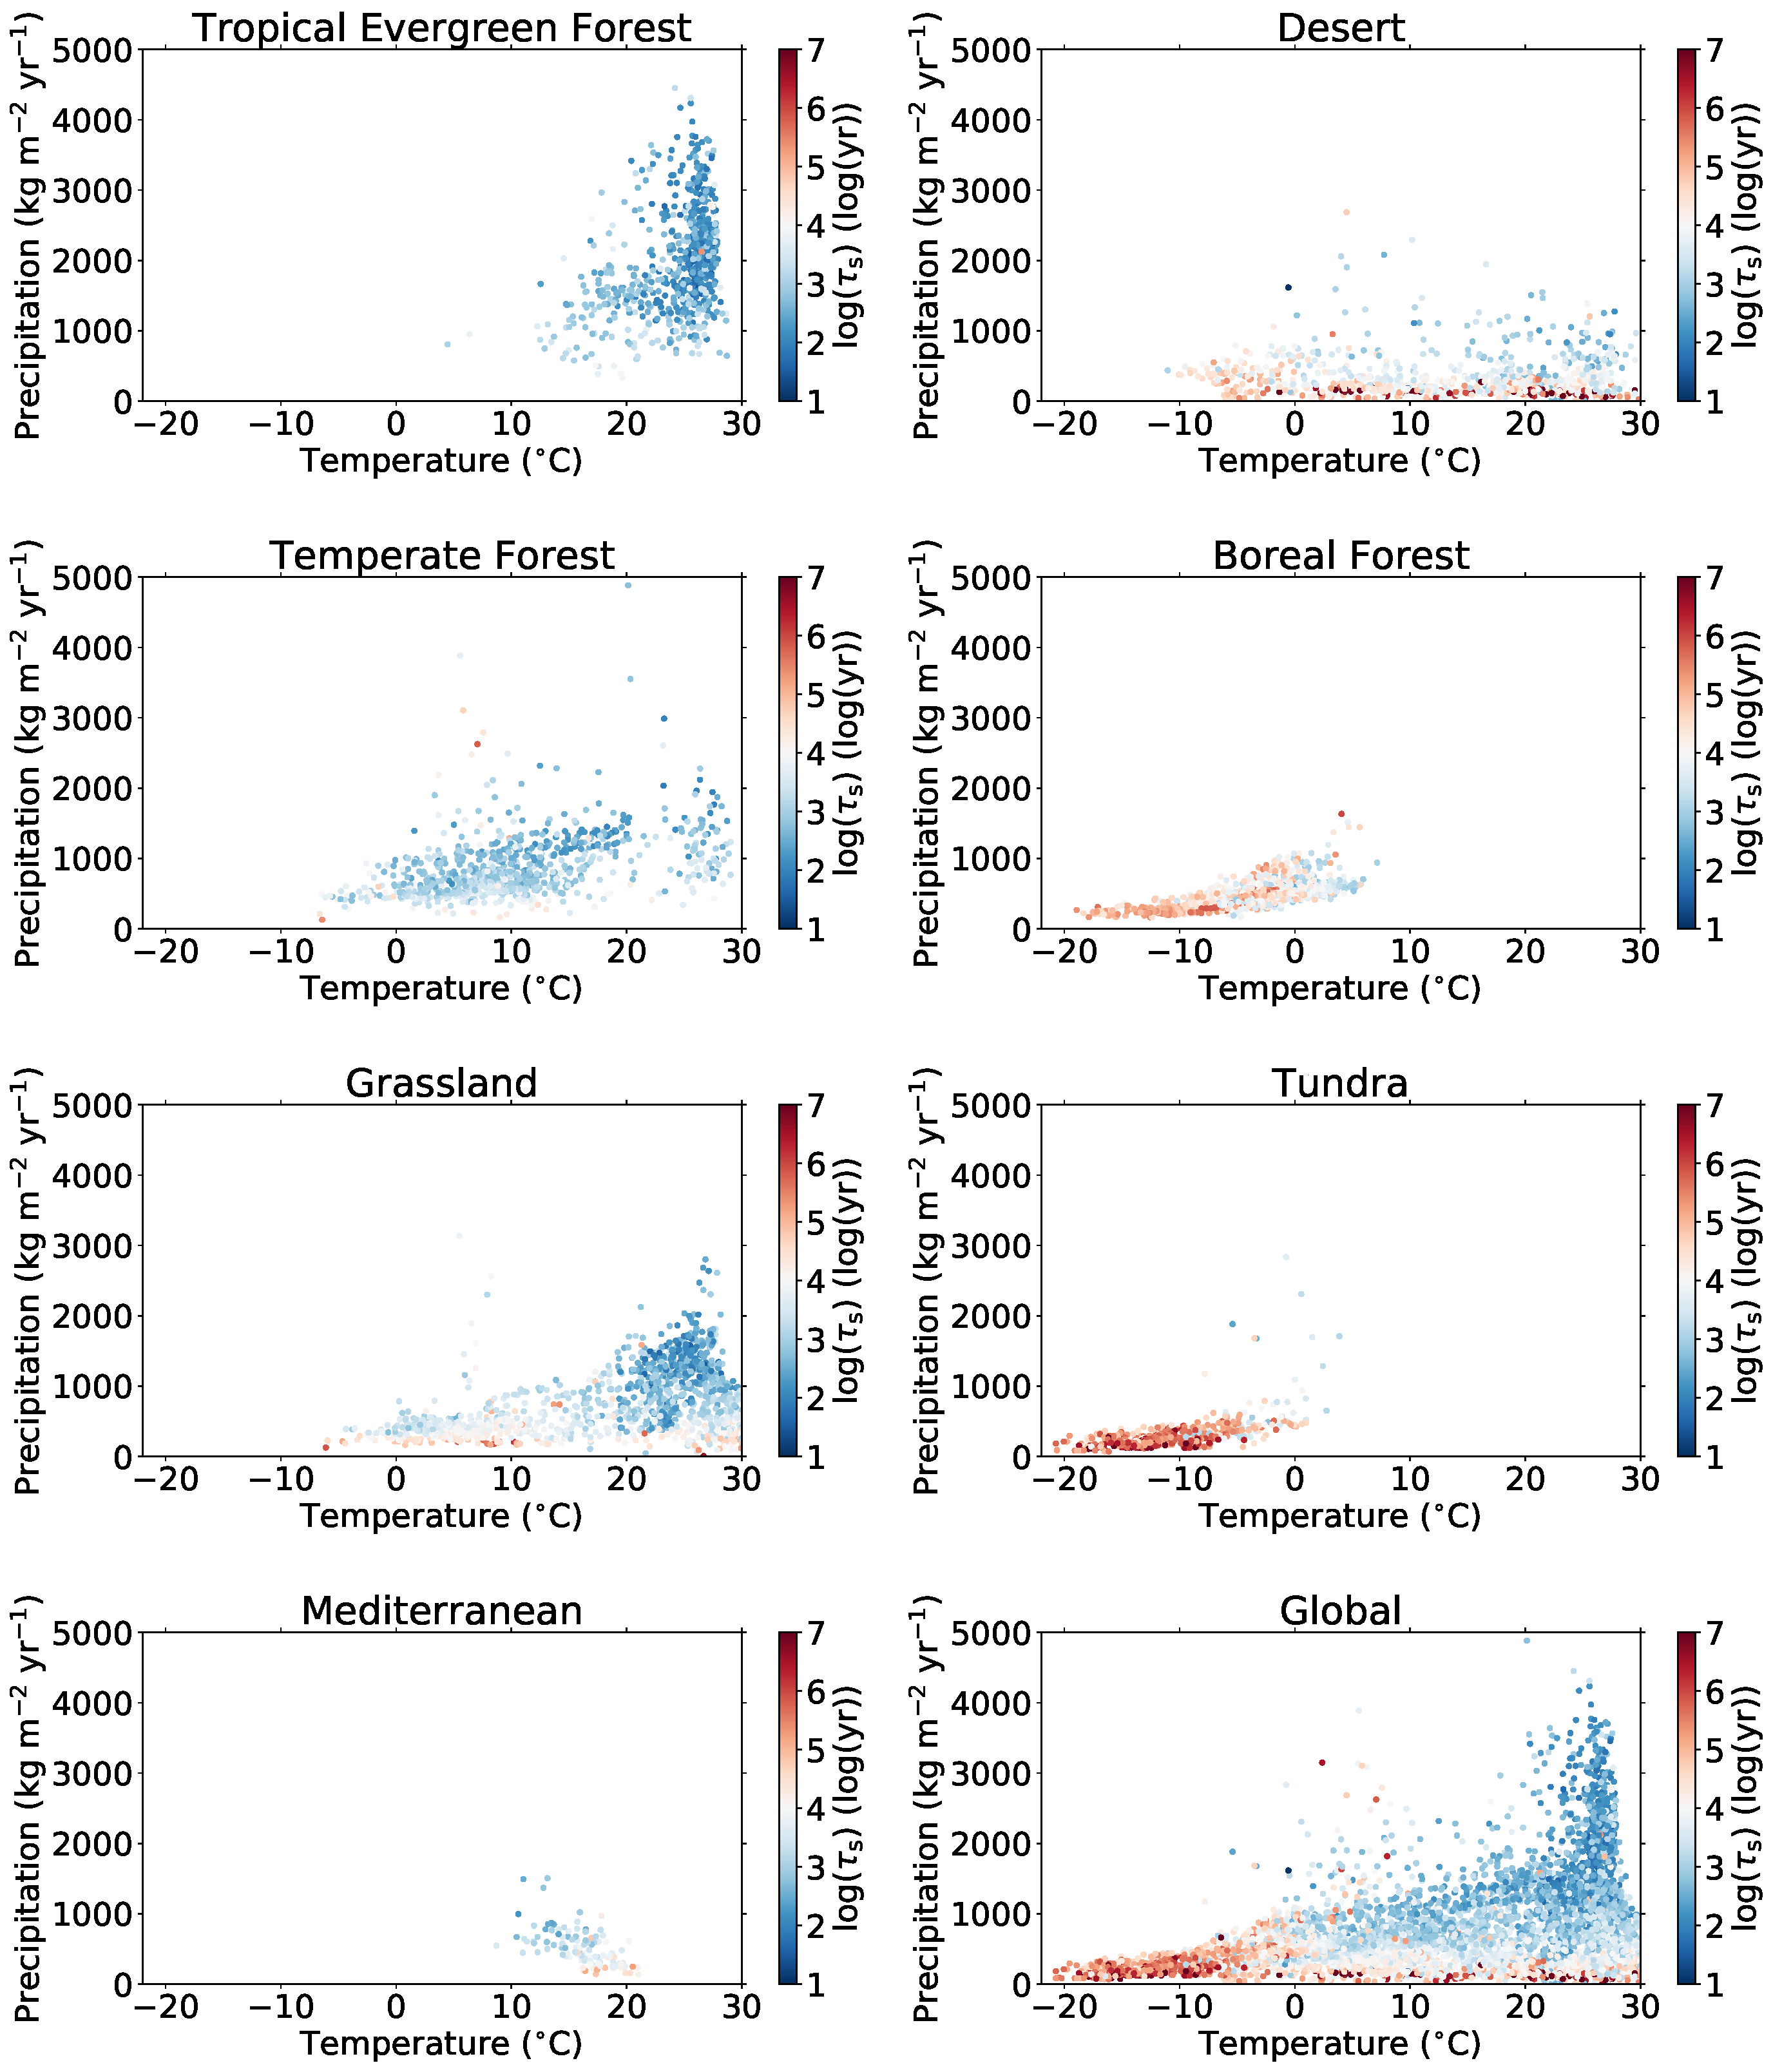
\includegraphics[width=6cm]{figs/Turnover/soil_obs1_colouredbytau_biome.pdf}
    \caption{Soil turnover \label{fig:EcoTurnoverlScatter}}
\end{figure*}

\hilight{Doug - add in SW maps}





\subsection{Drivers}
\hilight{Chantelle - Which figures to inlcude?}
\begin{figure*}[t]
    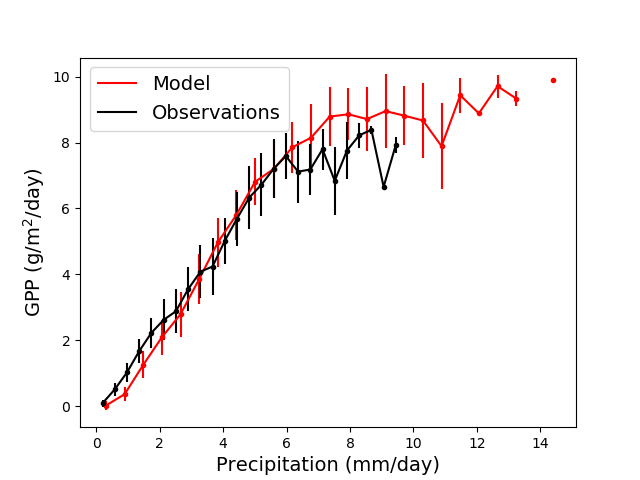
\includegraphics[width=6cm]{figs/GPPresponse/tl.png}
    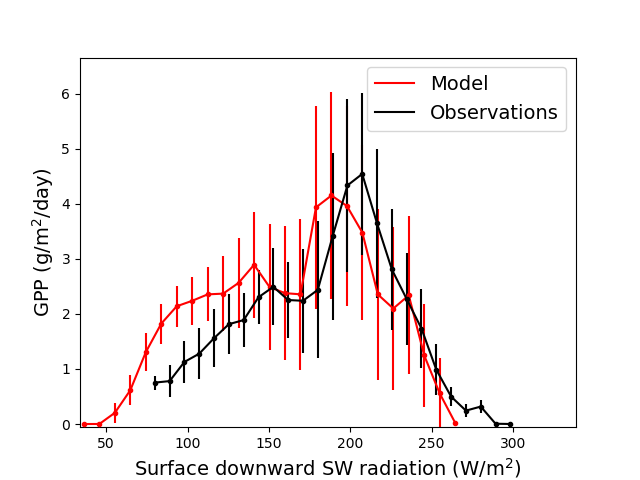
\includegraphics[width=6cm]{figs/GPPresponse/tr.png}
    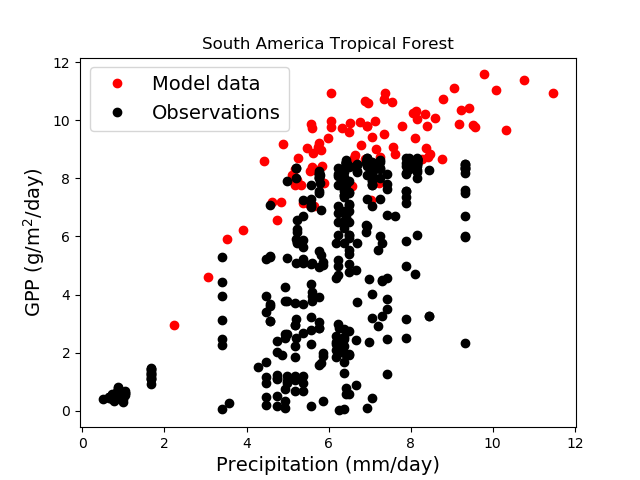
\includegraphics[width=6cm]{figs/GPPresponse/ml.png}
    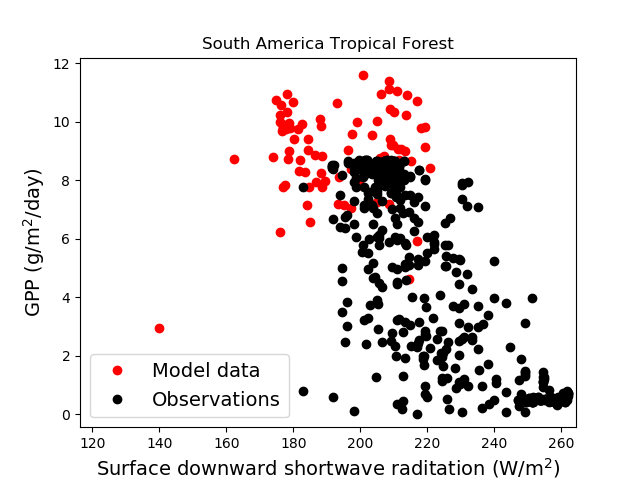
\includegraphics[width=6cm]{figs/GPPresponse/mr.png}
    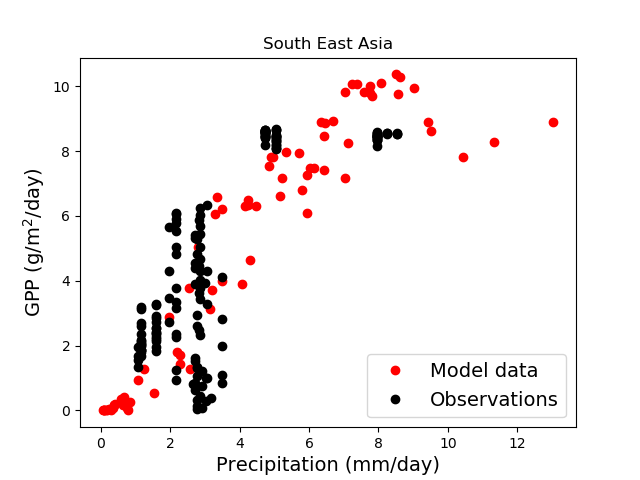
\includegraphics[width=6cm]{figs/GPPresponse/bl.png}
    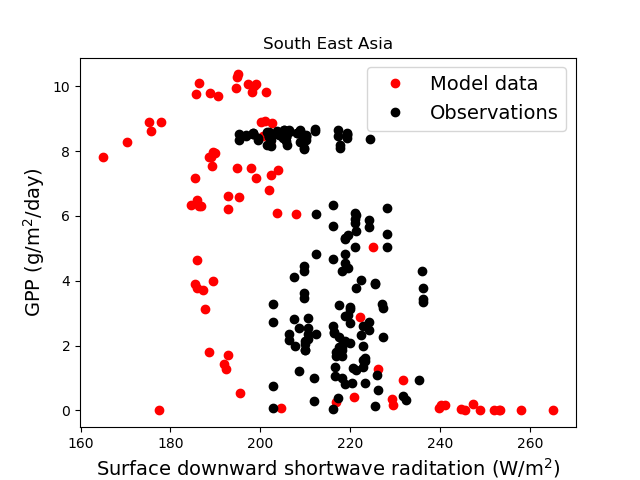
\includegraphics[width=6cm]{figs/GPPresponse/br.png}
    \caption{Response of GPP to precipitation (left column) and surface downward shortwave radiation (right column), for 1982-2008 ensemble mean. Top row shows global analysis, binned by independent variable (x). Data points show the mean, error bars show standard deviation range. Second and third rows show all data points for South America tropical forest, and South East Asia respectively. Observations are from GBAF (GPP), CERES (SWR), and GPCP2 (precipitation). \label{fig:GPPresponses}}
\end{figure*}

\hilight{Doug - add in new veg distribution scatter plots}

\begin{figure}[t]
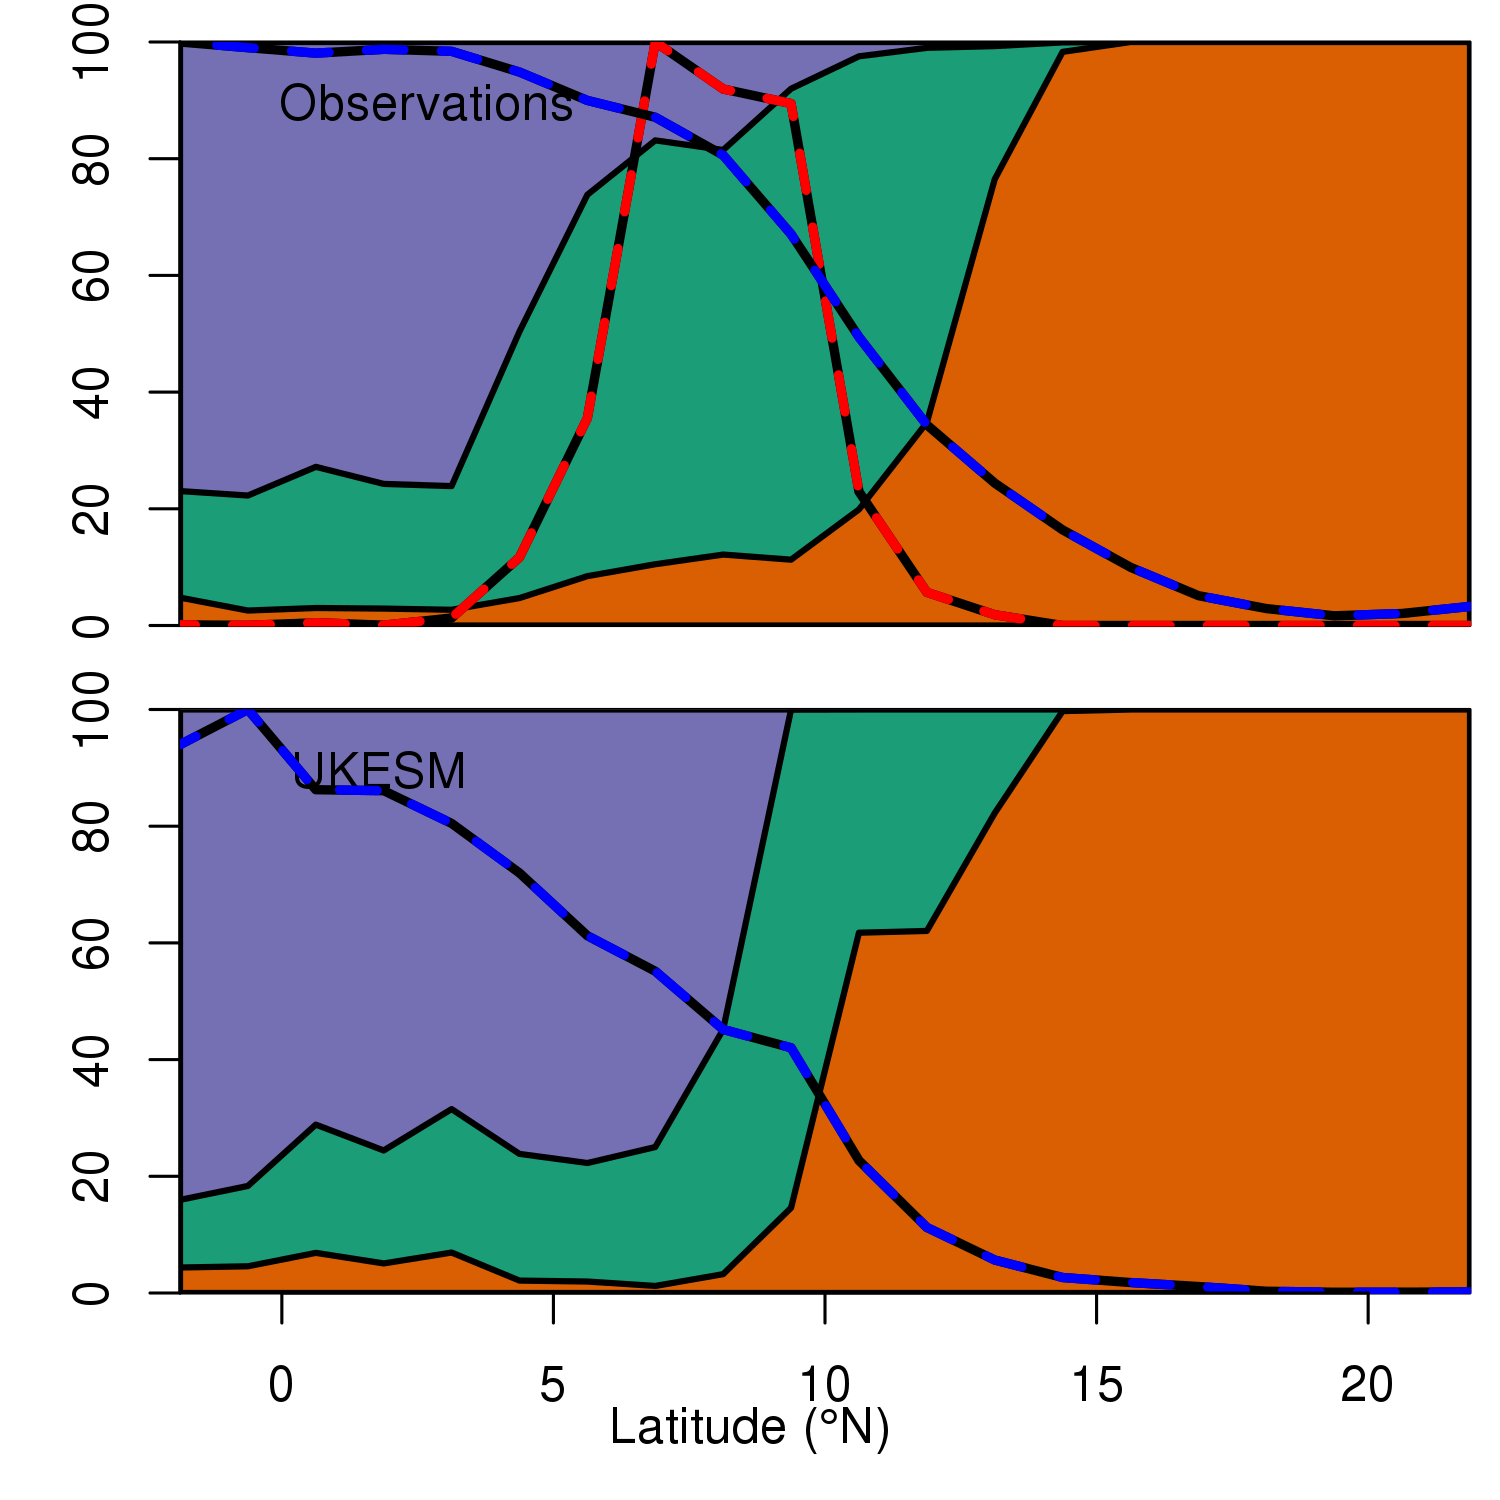
\includegraphics[width=8.3cm]{figs/trasect_AFRICA.png}
\caption{Transect of vegetation distribution from VCF observations and UKESM ensemble member u-bc179 along the longitude line of xx, spanning central Congo to central Sahara. Purple represents distribution of trees, green grasses and orange bare ground. Blue dotted line is observed mean annual precipitation from CRUTS 4.01 and u-bc179. Red dotted line is observed annual burnt area from GFED4s}
\end{figure}

\subsubsection{wetlands}
Generally good agreement is found between the two datasets, with large observed wetland fractions in the boreal regions reproduced in the model simulations. The tropical band of increased wetland fraction is found to be broader in the UKESM simulations than in the observations, particularly south of the Equator. We attribute much of this to a lack of tropical soils properties \citep{Gedney2019}.

Wetland methane emissions are primarily controlled by water table depth, temperature and available substrate. As such, adequately simulating the contemporary wetland area is important for modelling the methane cycle.  

\begin{figure*}[t]
    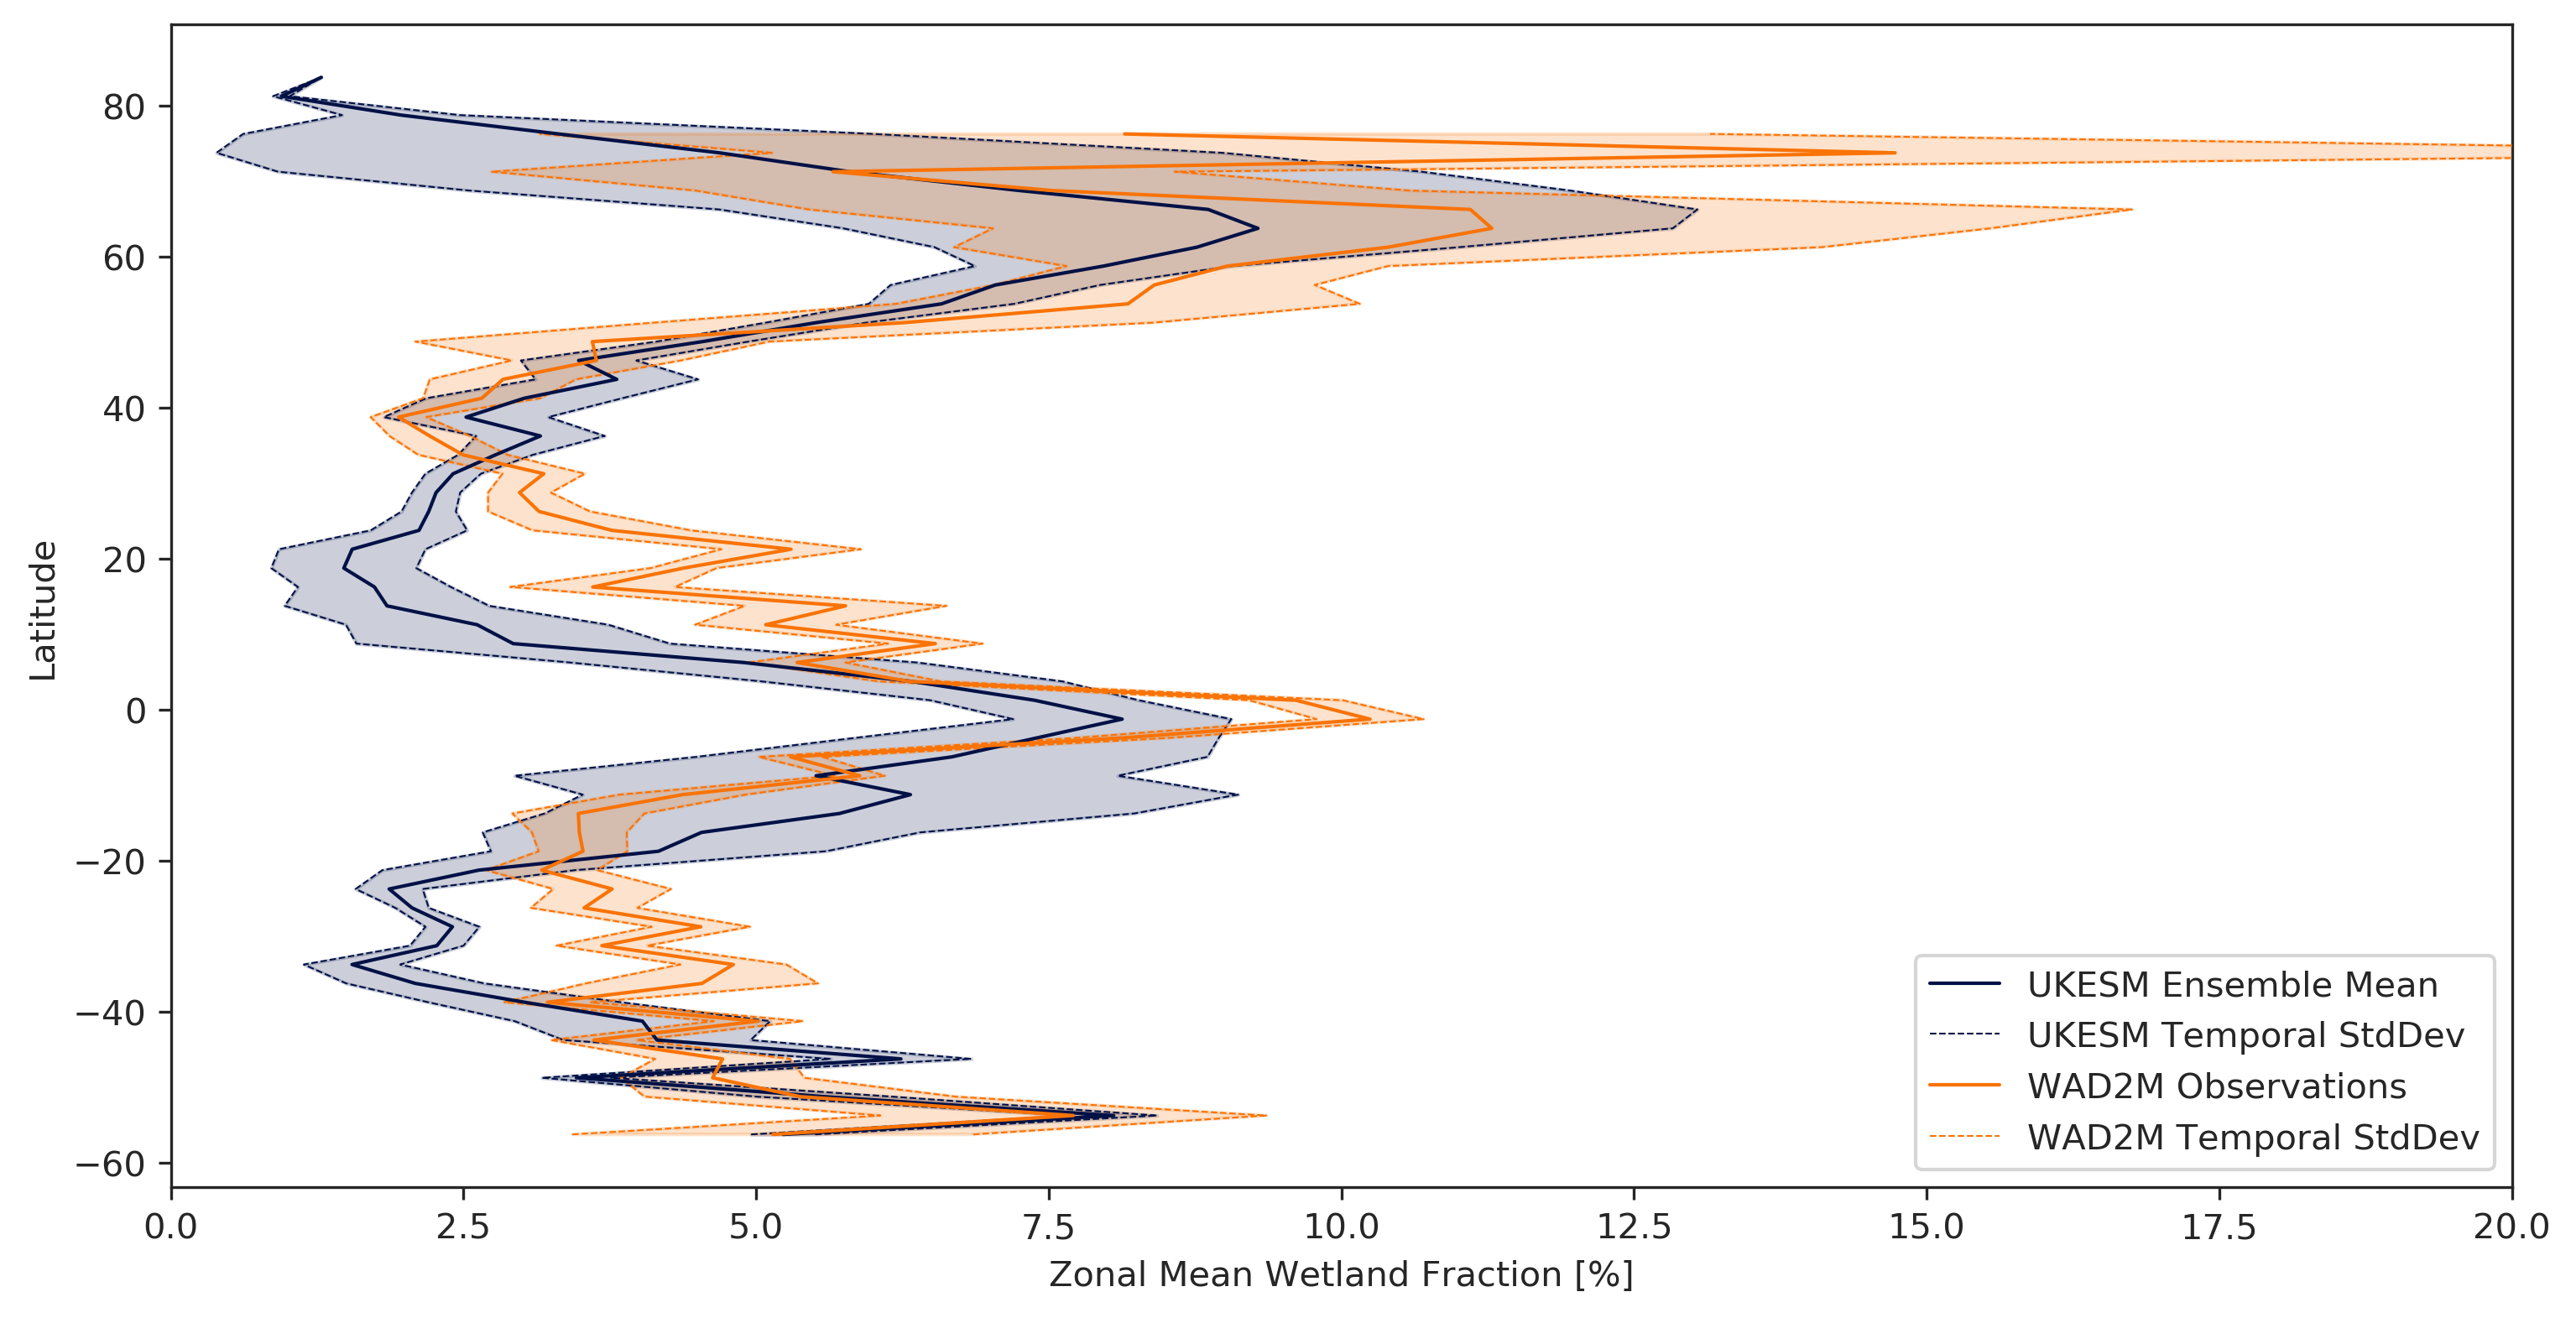
\includegraphics[width=16cm]{figs/Wetland.png}
    \caption{Zonal means in wetland extent for UKESM and observation.  \label{fig:wetland} }
\end{figure*}

\subsubsection{River flow}
There is a strong correlation with the multi-annual river flow (figure ***) \hilight{add figure} and obtain a correlation coefficient between modelled and observed for the multi-annual mean and log of river flow are 0.96 and 0.84 respectively. If we compare this to a similar off-line run where JULES is forced with observations we obtain correlation coefficients of 0.97 and 0.85 respectively, indicating that on a multi-year time scale UKESM is reproducing river flow well overall across the globe.
